\documentclass{mimosis}
\usepackage{metalogo}
\usepackage{pgf}
\usepackage{pgfplots}
\usepackage{fontawesome}
\usepackage{hepnicenames}
\usepackage{relsize}
\usepackage{pythonhighlight}
\usepackage{wrapfig}
\usepackage{scalerel}
\usepackage{mdframed}
\usepackage{bm}
\usepackage{multicol}
\usepackage{rotating}
\usepackage{pdfpages}
\usepackage{blindtext}
\usepackage[activate={true,nocompatibility},final,tracking=true, factor=1050,stretch=10,shrink=10]{microtype}
\SetTracking{encoding={*}, shape=sc}{40}


\RedeclareSectionCommand[
  tocpagenumberformat=\textbf
]{chapter}

\RedeclareSectionCommand[
  tocpagenumberformat=\textbf
]{part}

% \overfullrule=2mm

\usepackage{listings}

%%%%%%%%%%%%%%%%%%%%%%%%%%%%%%%%%%%%%%%%%%%%%%%%%%%%%%%%%%%%%%%%%%%%%%%%
% caption settings
%%%%%%%%%%%%%%%%%%%%%%%%%%%%%%%%%%%%%%%%%%%%%%%%%%%%%%%%%%%%%%%%%%%%%%%%
\captionsetup{font=small, labelfont=bf, format=plain}


\DeclareSIUnit\px{px}
\DeclareSIUnit\year{yr}
\DeclareSIUnit\century{century}
\DeclareSIUnit\lightyear{ly}
\DeclareSIUnit\gauss{G}

%%%%%%%%%%%%%%%%%%%%%%%%%%%%%%%%%%%%%%%%%%%%%%%%%%%%%%%%%%%%%%%%%%%%%%%%
% Fonts
%%%%%%%%%%%%%%%%%%%%%%%%%%%%%%%%%%%%%%%%%%%%%%%%%%%%%%%%%%%%%%%%%%%%%%%%

\setmainfont{Minion Pro}
\newfontfamily{\lstsansserif}[Scale=0.9,LetterSpace=0.0]{Fira Code}

\lstdefinelanguage{yaml}{
  keywords={true,false,null,y,n},
  keywordstyle=\color{darkgray}\bfseries,
  ndkeywordstyle=\color{black}\bfseries,
  literate={*}{{\lstsansserif*}}1,
  % identifierstyle=\color{black},
  sensitive=false,
  comment=[l]{\#},
  commentstyle=\color{gray}\ttfamily,
  moredelim=[l][\color{orange}]{\&},
  % stringstyle=\color{blue}\ttfamily,
}



%%%%%%%%%%%%%%%%%%%%%%%%%%%%%%%%%%%%%%%%%%%%%%%%%%%%%%%%%%%%%%%%%%%%%%%%
% Bibliography
%%%%%%%%%%%%%%%%%%%%%%%%%%%%%%%%%%%%%%%%%%%%%%%%%%%%%%%%%%%%%%%%%%%%%%%%
%
% I like the bibliography to be extremely plain, showing only a numeric
% identifier and citing everything in simple brackets. The first names,
% if present, will be initialized. DOIs and URLs will be preserved.

\usepackage[%
autocite     = plain,
backend      = biber,
doi          = true,
eprint       = true,
url          = true,
giveninits   = true,
hyperref     = true,
% isbn         = false,
maxbibnames  = 300,
maxcitenames = 300,
maxnames     = 5,
sortcites    = true,
style        = numeric,
]{biblatex}

\setlength\bibitemsep{0.8\baselineskip}
\patchcmd{\bibsetup}{\interlinepenalty=5000}{\interlinepenalty=10000}{}{} % no break of entr
%%%%%%%%%%%%%%%%%%%%%%%%%%%%%%%%%%%%%%%%%%%%%%%%%%%%%%%%%%%%%%%%%%%%%%%%
% Some adjustments to make the bibliography more clean
%%%%%%%%%%%%%%%%%%%%%%%%%%%%%%%%%%%%%%%%%%%%%%%%%%%%%%%%%%%%%%%%%%%%%%%%
%
% The subsequent commands do the following:
%  - Removing the month field from the bibliography
%  - Fixing the Oxford commma
%  - Suppress the "in" for journal articles
%  - Remove the parentheses of the year in an article
%  - Delimit volume and issue of an article by a colon ":" instead of
%    a dot ""
%  - Use commas to separate the location of publishers from their name
%  - Remove the abbreviation for technical reports
%  - Display the label of bibliographic entries without brackets in the
%    bibliography
%  - Ensure that DOIs are followed by a non-breakable space
%  - Use hair spaces between initials of authors
%  - Make the font size of citations smaller
%  - Fixing ordinal numbers (1st, 2nd, 3rd, and so) on by using
%    superscripts

% Remove the month field from the bibliography. It does not serve a good
% purpose, I guess. And often, it cannot be used because the journals
% have some crazy issue policies.
\AtEveryBibitem{\clearfield{month}}
\AtEveryCitekey{\clearfield{month}}
\renewcommand*\finentrypunct{}
\DeclareSourcemap{
  \maps[datatype=bibtex]{
     \map{
        \step[fieldsource=doi,final]
        \step[fieldset=isbn,null]
        }
      }
}

\DeclareSourcemap{
  \maps[datatype=bibtex]{
    \map{
      \step[fieldsource=note, final]
      \step[fieldset=addendum, origfieldval, final]
      \step[fieldset=note, null]
    }
  }
}


\DeclareSourcemap{
 \maps[datatype=bibtex,overwrite=true]{
  \map{
    \step[fieldsource=Collaboration, final=true]
    \step[fieldset=usera, origfieldval, final=true]
  }
 }
}

\renewbibmacro*{author}{%
  \iffieldundef{usera}{%
    \printnames{author}%
  }{%
    \printnames{author} (\printfield{usera} Collaboration)%
  }%
}%

% Fixing the Oxford comma. Not sure whether this is the proper solution.
% More information is available under [1] and [2].
%
% [1] http://tex.stackexchange.com/questions/97712/biblatex-apa-style-is-missing-a-comma-in-the-references-why
% [2] http://tex.stackexchange.com/questions/44048/use-et-al-in-biblatex-custom-style
%
\AtBeginBibliography{%
  \renewcommand*{\finalnamedelim}{%
    \ifthenelse{\value{listcount} > 2}{%
      \addcomma
      \addspace
      \bibstring{and}%
    }{%
      \addspace
      \bibstring{and}%
    }
  }
}

% Suppress "in" for journal articles. This is unnecessary in my opinion
% because the journal title is typeset in italics anyway.
\renewbibmacro{in:}{%
  \ifentrytype{article}
  {%
  }%
  % else
  {%
    \printtext{\bibstring{in}\intitlepunct}%
  }%
}

% Remove the parentheses for the year in an article. This removes a lot
% of undesired parentheses in the bibliography, thereby improving the
% readability. Moreover, it makes the look of the bibliography more
% consistent.
\renewbibmacro*{issue+date}{%
  \setunit{\addcomma\space}
    \iffieldundef{issue}
      {\usebibmacro{date}}
      {\printfield{issue}%
       \setunit*{\addspace}%
       \usebibmacro{date}}%
  \newunit}

% Delimit the volume and the number of an article by a colon instead of
% by a dot, which I consider to be more readable.
\renewbibmacro*{volume+number+eid}{%
  \printfield{volume}%
  \setunit*{\addcolon}%
  \printfield{number}%
  \setunit{\addcomma\space}%
  \printfield{eid}%
}

% Do not use a colon for the publisher location. Instead, connect
% publisher, location, and date via commas.
\renewbibmacro*{publisher+location+date}{%
  \printlist{publisher}%
  \setunit*{\addcomma\space}%
  \printlist{location}%
  \setunit*{\addcomma\space}%
  \usebibmacro{date}%
  \newunit%
}

% Ditto for other entry types.
\renewbibmacro*{organization+location+date}{%
  \printlist{location}%
  \setunit*{\addcomma\space}%
  \printlist{organization}%
  \setunit*{\addcomma\space}%
  \usebibmacro{date}%
  \newunit%
}

% Do not abbreviate "technical report".
\DefineBibliographyStrings{english}{%
  techreport = {technical report},
}

% Display the label of a bibliographic entry in bare style, without any
% brackets. I like this more than the default.
%
% Note that this is *really* the proper and official way of doing this.
\DeclareFieldFormat{labelnumberwidth}{#1\adddot}


% \renewbibmacro*{doi+eprint+url}{%
%   \setunit{\addspace}\newblock
%   \scriptsize%
%   \iftoggle{bbx:doi}
%     {\printfield{doi}}
%     {}%
%   \setunit{\addspace}\newblock
%   \iftoggle{bbx:eprint}
%     {\usebibmacro{eprint}}
%     {}%
%   \setunit{\addspace}\newblock
%   \iftoggle{bbx:url}
%     {\usebibmacro{url+urldate}}
%     {}
% }


% Ensure that DOIs are followed by a non-breakable space.
\DeclareFieldFormat{doi}{%
  \newline
  \scriptsize%
  \mkbibacro{DOI}\addcolon\addnbspace
  {\href{http://dx.doi.org/#1}{\nolinkurl{#1}}}
}

\DeclareFieldFormat{addendum}{%
  \newline
  \scriptsize%
  {\color{gray}{Note\addcolon\addnbspace#1}}
}

\DeclareFieldFormat{urldate}{%
  \scriptsize%
  {\color{gray}{visited on #1}}
}


% \DeclareFieldFormat{eprint}{%
%   \newline
%   \scriptsize%
%   \mkbibacro{DOI}\addcolon\addnbspace
%     \ifhyperref
%       {\href{http://dx.doi.org/#1}{\nolinkurl{#1}}}
%       %
%       {\nolinkurl{#1}}
% }

\DeclareFieldFormat{eprint:arxiv}{%
  \scriptsize%
  \iffieldundef{doi}
  {\newline}
  {}
  \mkbibacro{arXiv}\addcolon\addnbspace%
  \ifhyperref
    {\href{https://arxiv.org/abs/#1}{\nolinkurl{#1}}
    \iffieldundef{eprintclass}
    {}
    {\href{https://arxiv.org/abs/#1}{[{\nolinkurl{\thefield{eprintclass}}}]}}
    }
    {\nolinkurl{#1}}
}


% Ensure that URLS appear on a newline 
\DeclareFieldFormat{url}{%
\newline
\scriptsize%
{\url{#1}}
}


\DefineBibliographyStrings{english}{%
  pages = {pages},
  page = {page},
}

% Use proper hair spaces between initials as suggested by Bringhurst and
% others.
\renewcommand*\bibinitdelim{\addnbthinspace}
\renewcommand*\bibnamedelima{\addnbthinspace}
\renewcommand*\bibnamedelimb{\addnbthinspace}
\renewcommand*\bibnamedelimi{\addnbthinspace}

% Make the font size of citations smaller. Depending on your selected
% font, you might not need this.
\renewcommand*{\citesetup}{%
  \biburlsetup
  \small
}

% \DeclareLanguageMapping{british}{bibliography-correct-ordinals}
% \DeclareLanguageMapping{english}{bibliography-correct-ordinals}

\bibliography{thesis}


\makeglossaries

%%%%%%%%%%%%%%%%%%%%%%%%%%%%%%%%%%%%%%%%%%%%%%%%%%%%%%%%%%%%%%%%%%%%%%%%
%software names
%%%%%%%%%%%%%%%%%%%%%%%%%%%%%%%%%%%%%%%%%%%%%%%%%%%%%%%%%%%%%%%%%%%%%%%%
\newcommand{\gammapy}{\texttt{gammapy}\xspace}
\newcommand{\naima}{\texttt{naima}\xspace}
\newcommand{\emcee}{\texttt{emcee}\xspace}
\newcommand{\python}{Python\xspace}
\newcommand{\java}{Java\xspace}
\newcommand{\corsika}{CORSIKA\xspace}
\newcommand{\simtel}{\texttt{sim\_telarray}\xspace}
\newcommand{\numpy}{\texttt{numpy}\xspace}
\newcommand{\scipy}{\texttt{scipy}\xspace}
\newcommand{\mars}{\texttt{MARS}\xspace}
\newcommand{\eventdisplay}{\texttt{Eventdisplay}\xspace}
\newcommand{\sklearn}{\texttt{scikit-learn}\xspace}
\newcommand{\rootcern}{\texttt{ROOT}\xspace}
\newcommand{\ctapipe}{\texttt{ctapipe}\xspace}
\newcommand{\astropy}{\texttt{astropy}\xspace}
\newcommand{\matplotlib}{\texttt{matplotlib}\xspace}
\newcommand{\aicttools}{\texttt{aict-tools}\xspace}
\newcommand{\pandas}{\texttt{pandas}\xspace}
\newcommand{\hdf}{\texttt{HDF5}\xspace}
\newcommand{\yaml}{\texttt{yaml}\xspace}
\newcommand{\ctaplots}{\texttt{ctaplots}\xspace}
\newcommand{\jayct}{\texttt{jayct}\xspace}
\newcommand{\flink}{\texttt{flink}\xspace}
\newcommand{\make}{\texttt{make}\xspace}
\newcommand{\snakemake}{\texttt{snakemake}\xspace}
% \newcommand{\scikit-learn}{\texttt{scikit-learn}\xspace}
\newcommand{\pymc}{\texttt{PyMC3}\xspace}
\newcommand{\theano}{\texttt{Theano}\xspace}
\newcommand{\pytorch}{\texttt{PyTorch}\xspace}
\newcommand{\tensorflow}{\texttt{Tensorflow}\xspace}
% open gamma-ray astro format abbreviation
\newcommand{\oga}{OGA\xspace}

\newcommand{\cuda}{CUDA\xspace}

\newcommand{\ssclong}{Synchrotron Self-Compton\xspace}
% \newcommand{\scipy}{\texttt{scipy}\xspace}
\newcommand{\cpp}{C\nolinebreak\hspace{-.05em}\raisebox{.3ex}{\relsize{-2}{\textbf{+}}}\nolinebreak\hspace{-.10em}\raisebox{.3ex}{\relsize{-2}{\textbf{+}}}\xspace}

%%%%%%%%%%%%%%%%%%%%%%%%%%%%%%%%%%%%%%%%%%%%%%%%%%%%%%%%%%%%%%%%%%%%%%%%
% telescope names
%%%%%%%%%%%%%%%%%%%%%%%%%%%%%%%%%%%%%%%%%%%%%%%%%%%%%%%%%%%%%%%%%%%%%%%%
\newcommand{\magic}{MAGIC\xspace}
\newcommand{\fact}{FACT\xspace}
\newcommand{\hess}{H.E.S.S.\xspace}
\newcommand{\hegra}{HEGRA\xspace}
\newcommand{\veritas}{VERITAS\xspace}
\newcommand{\whipple}{WHIPPLE\xspace}
\newcommand{\fermilat}{Fermi-LAT\xspace}
\newcommand{\fermi}{Fermi\xspace}
\newcommand{\kascade}{KASCADE\xspace}


%%%%%%%%%%%%%%%%%%%%%%%%%%%%%%%%%%%%%%%%%%%%%%%%%%%%%%%%%%%%%%%%%%%%%%%%
% math and variables
%%%%%%%%%%%%%%%%%%%%%%%%%%%%%%%%%%%%%%%%%%%%%%%%%%%%%%%%%%%%%%%%%%%%%%%%
\newcommand{\etrue}{E_T\xspace}
\newcommand{\eest}{E_\text{Est}\xspace}
\newcommand{\Non}{N_\text{on}\xspace}
\newcommand{\Noff}{N_\text{off}\xspace}
\newcommand{\tobs}{t_{\text{obs}}\xspace}
\newcommand{\talpha}{t_{\alpha}\xspace}

\newcommand{\norm}[1]{\left\lVert#1\right\rVert}
\newcommand{\edisp}{\mathbf{p_D}\xspace}
\newcommand{\aeff}{A_\text{eff}\xspace}
\newcommand{\ddp}[1]{\frac{\partial}{\partial #1}}
\newcommand{\dddp}[2]{\frac{\partial #1}{\partial #2}}
% \newcommand*{\annot}[1]{\tag*{\footnotesize{\textcolor{black!50}{#1}}}}
\newcommand{\erf}{\operatorname{erf}}
\newcommand{\github}[1]{\url{https://github.com/#1}~\faGithub}
\newenvironment{nscenter}
 {\parskip=0.7em\par\nopagebreak\centering}
 {\par\noindent\ignorespacesafterend}
\newcommand{\githubcenter}[1]{
  \begin{nscenter}
  \url{https://github.com/#1}~\faGithub
  \end{nscenter}
}



\renewcommand*{\partpagestyle}{empty}

%%%%%%%%%%%%%%%%%%%%%%%%%%%%%%%%%%%%%%%%%%%%%%%%%%%%%%%%%%%%%%%%%%%%%%%%
% useful stuff
%%%%%%%%%%%%%%%%%%%%%%%%%%%%%%%%%%%%%%%%%%%%%%%%%%%%%%%%%%%%%%%%%%%%%%%%
\newcommand\numberthis{\addtocounter{equation}{1}\tag{\theequation}} %% https://tex.stackexchange.com/questions/42726/align-but-show-one-equation-number-at-the-end




\hyphenation{Che-ren-kov}
\hyphenation{Gravi-tational}

%%%%%%%%%%%%%%%%%%%%%%%%%%%%%%%%%%%%%%%%%%%%%%%%%%%%%%%%%%%%%%%%%%%%%%%%
% glossary and abbreviations
%%%%%%%%%%%%%%%%%%%%%%%%%%%%%%%%%%%%%%%%%%%%%%%%%%%%%%%%%%%%%%%%%%%%%%%%


\RedeclareSectionCommand[tocnumwidth=1.5em]{part}
\RedeclareSectionCommand[tocnumwidth=1.5em]{chapter}
\RedeclareSectionCommand[tocnumwidth=2.1em]{section}


\renewcommand*{\coverpagetopmargin}{0mm}
\renewcommand*{\coverpageleftmargin}{0mm}
\renewcommand*{\coverpagerightmargin}{0mm}
\renewcommand*{\coverpagebottommargin}{0mm}

\setcounter{tocdepth}{1}
%%%%%%%%%%%%%%%%%%%%%%%%%%%%%%%%%%%%%%%%%%%%%%%%%%%%%%%%%%%%%%%%%%%%%%%%
% Incipit
%%%%%%%%%%%%%%%%%%%%%%%%%%%%%%%%%%%%%%%%%%%%%%%%%%%%%%%%%%%%%%%%%%%%%%%%

\begin{document}

\frontmatter

\includepdf{build/titlepage.pdf}
% \selectlanguage{ngerman}

\begin{titlepage}
	\begin{center}
		\textsc{\huge Inauguraldissertation}
                \vskip 1cm
                \begin{large}
                  zur Erlangung der Doktorwürde der\\[0.50cm]
                  \begin{Large}
                    \textsc{Fakultät für Physik}\\[0.50cm]
                  \end{Large}
                  der\\[0.50cm]
                  \begin{Large}
                    \textsc{Technische Universität Dortmund}\par
                  \end{Large}
                \end{large}
		%
		\vfill
		%
		\begin{large}
                  vorgelegt von\\
                  M.Sc. Physik\\[0.5cm]
                  \begin{LARGE}
                    \textbf{Kai Brügge}
                  \end{LARGE}\\[0.5cm]
                  aus Dortmund
		\end{large}
    %
    \vskip 1cm
    %
    % \begin{small}
    %   Tag der mündlichen Prüfung: 01.01.1954
    % \end{small}
	\end{center}
\end{titlepage}

\selectlanguage{english}

\begin{titlepage}
  %
  \phantom{}
  \vfill 
  %
  \begin{center}
    \begin{singlespace*}
      \begin{Huge}
          Persistent Homology in\\
          Multivariate Data Visualization\par
      \end{Huge}
      %
      \vskip 0.25cm
      \emph{by}
      \vskip 0.25cm
      %
      \textsc{Kai Brügge}\par
    \end{singlespace*}
  \end{center}
  %
  \vfill
  %
  \begin{singlespace*}
    Supervisors:            Prof.\,Dr.\, Dr.\, Wolfgang Rhode\\
    \phantom{Supervisors:}  Prof.\,Dr.\, Kevin Kröninger
  \end{singlespace*}
\end{titlepage}

\newpage
\null
\thispagestyle{empty}
\newpage

\newpage
\null
\thispagestyle{empty}
% \newpage
% \newpage
\begin{center}
  \large{Abstract}
\end{center}
%
\noindent

% This text deals with the data analysis process of imaging atmospheric Cherenkov telescopes (IACT) with a focus on reproducibility and open-source solutions.
Imaging atmospheric Cherenkov telescopes (IACT) observe the sky in the highest energy ranges. 
% These telescopes capture gamma rays originating in the most extreme environments in the universe. 
From the remnants of cataclysmic supernovae to jets powered by supermassive blackholes in the center of distant galaxies,
IACTs can capture the light emerging from the most extreme sources in the universe. 

% The first part of my thesis mainly deals with the creation of energy spectra of point-sources as observed by IACTs.
With the recent advent of multi-messenger astronomy it has become critical for IACTs to publicly share their data and software.
% The first part of my thesis motivates the need for a common description of instrument response functions and event lists 
For the first time since the inception of IACT technology, in a combined effort of the \hess, \magic, \veritas, and \fact collaborations,
observations of the Crab Nebula were made available to the general public in a common data format. 
The first part of my thesis demonstrates the viability of the common data format 
by performing a spectral analysis of the Crab Nebula on the published datasets.
% The majority of the text deals with the computation of energy spectra and flux-point estimates from this common dataset. 
% of the Crab Nebula and 
% The text aims to work as an introduction for the uninitiated reader and tries to collect and formalize
% 
The text gives detailed descriptions and mathematical formalizations of instrument response functions (IRFs) and the statistical 
modeling used for typical spectral analyses. This is essential to understand the measurement process of IACTs. 
The ultimate goal of this part of the thesis will be to use Hamilton Markov Monte Carlo methods 
to test spectral models and unfold flux-point estimates for the Crab Nebula.

The common data format paves the road for the operation of the upcoming Cherenkov Telescope Array (CTA).
Once CTA has been constructed, it will be the largest and most sophisticated experiment in the field of ground-based gamma-ray astronomy.
It will be operated as an open observatory allowing anyone to access the recorded data.
The second part of my thesis concentrates on reproducible analysis for the Cherenkov Telescope Array (CTA).
Once operational, CTA will produce a substantial amount of data creating new challenges for data storage and analysis technologies.
In this part of the thesis I use simulated CTA data to build a comprehensive analysis chain based on fully open-source methods.
The goal is to create a pipeline that rivals the physics performance of CTA's closed-source reference implementation.
Every step of the analysis, from raw-data processing to the calculation of sensitivity curves,
will be optimized with respect to complexity, reproducibility and run-time.

% % \section{Thesis Contents and Current Progress}

% My thesis deals with the data analysis process of imaging atmospheric Cherenkov telescopes (IACT) under resource constraints
% with a focus on reproducibility.
% For my thesis I use simulated data of the CTA experiment to build an exhaustive analysis chain based on open-source software and
% reproducible methods. Every step of the analysis, from raw-data processing to estimation of spectral energy densities,
% will be optimized with respect to real-time constraints, complexity, and reproducibility.
% All methods and algorithms will be tested using open data from the currently operating Cherenkov telescopes


% The astroparticle community inhereted  many of its ideas and technologies from 
% In the first part of this thesis I lay out a way to perform high-level spectral analysis of IACT data using open-source programs and data formats.
% The Crab Nebula is the prototypical object of this kind. It is a steady source of bright TeV gamma-ray emission in the northern sky and is
% the model to data from six different experiments using Markov chain sampling. This empha- sizes the importance of open data in the Cherenkov astronomy community.
%  Without open access to flux data from multiple wavelengths, no model assumptions can be validated.
% Chapter 5 goes through the all the harrowing details needed in order to understand the measurement process of IACTs. 
% A critical part of which is the computation of the instrument response functions. In section 5.2 these response functions are formalized in an instrument agnostic way. 
% The ultimate goal of which, is the construction of a common data format that can be used by any IACT instrument.
%  Traditionally, all IACT collaborations use their own proprietary software and data formats to produce high-level results like flux points.
  % In a mutual endeavour between the MAGIC, H.E.S.S, VERITAS, and FACT collaborations to change the current state of affairs, a small data sample of Crab Nebula
  %  observations was made public in this common data format. Using this data we published the first joint and fully open-source analysis of combined IACT data [121]. 
  %  In section 5.6 I use the published event lists and instrument response functions to fit a log-parabolic spectral model to the IACT data using Hamilton Markov chain
    % sampling. Section 5.7 shows how that sa
% \todo{diesen Mist vernünftig schreiben}

% \begin{center}
%   \textsc{Kurzfassung}
% \end{center}
% %
% \noindent
% %

% \begin{german}
% Meine Thesis is hard am dealen.
% \end{german}

\KOMAoptions{open=left}
\tableofcontents
\KOMAoptions{open=right}

\mainmatter

\setpartpreamble[o]{%
\tikz[remember picture,overlay] \node[opacity=0.25,inner sep=150pt] at (current page.center){\includegraphics[width=0.9\paperwidth,height=0.9\paperheight]{figures/contours_mst.jpg}};%
}
\part{Open Cherenkov Astronomy}
%%%%%%%%%%%%%%%%%%%%%%%%%%%%%%%%%%%%%%%%%%%%%%%%%%%%%%%%%%%%%%%%%%%%%%%%
\chapter{Introduction}
%%%%%%%%%%%%%%%%%%%%%%%%%%%%%%%%%%%%%%%%%%%%%%%%%%%%%%%%%%%%%%%%%%%%%%%%

% Since the early days of the last century, scientists have been searching for the sources of cosmic radiation. 
The discovery of cosmic rays during the daring balloon flights of Victor Franz Hess in 1912~\cite{hess_original} opened up
an entirely new window into the universe.
This elusive radiation, which so relentlessly bombards us from outer space, carries a wealth of information
about the most violent processes in the cosmos. 
Probing the gamma-ray sky is crucial to understanding the processes which drive the cosmic-ray acceleration.
While charged cosmic rays are deflected by magnetic fields, gamma rays pinpoint back to the source and allow us to image these objects. 
Only the combination of data from multiple facilities can help to unravel the inner workings of
cosmic-ray sources. 
The success of these joint campaigns has become apparent recently through the first observational evidence
of neutrino emission from the blazar TXS 0506+056~\cite{icecube2018multimessenger}. 
This collective effort used data from the IceCube neutrino observatory in Antarctica as well as data from the gamma-ray 
experiments \fermi and \magic. 
From its very beginning, the \fermi collaboration made all of its recorded data and software available to the general public.
With the recent advent of multi-messenger astronomy it has become critical for imaging atmospheric Cherenkov telescopes (IACT)
to openly share their data as well.
This first part of my thesis deals mainly with the
computation of energy spectra and flux point estimates in an open and reproducible manner and tries to motivate the need for public IACT data. 
The text aims to convey all the essential information that is needed in order to understand the measurement process of IACTs. 
% The following chapters serve as a single comprehensive 
% The following chapters target the uninitiated reader 

The galactic cosmic ray population is seeded by remnants of cataclysmic supernova events.
The Crab Nebula is the prototypical object of this kind.  
It is a steady source of bright \si{TeV} gamma-ray emission in the northern sky and is 
continuously observed by radio, X-ray,  and gamma-ray observatories. 
It was the first gamma-ray source detected by an imaging atmospheric Cherenkov telescope (IACT) in 1989~\cite{whipple_crab}. 
In \cref{ch:theory} I describe the typical emission processes prevalent in supernova remnants (SNR) 
and describe how log-parabolic energy spectra emerge in many sources of cosmic rays.
\Cref{ch:observatories} gives an overview of experimental techniques used to observe gamma rays. 
In \cref{ch:crab-sed} I show that the spectral energy distribution of the Crab Nebula,  in an energy range from 
a few \si{keV} to tens of \si{TeV}, can be described with a single electron population of log-parabolic shape.
In that chapter I model the synchrotron, inverse Compton, and \ssclong emission using the \naima~\cite{naima} program
and fitted the model to data from six different experiments using Markov chain sampling. 
This emphasizes the importance of open data in the Cherenkov astronomy community.
Without open access to flux data from multiple wavelengths, no model assumptions can be validated. 
% The ultimate goal my thesis will be to propose a reproducible and open-source analysis chain 
% for IACTs.

\Cref{ch:spectral} goes through all the harrowing details needed in order to understand the
measurement process of IACTs, a critical part of which is the 
computation of the instrument response functions. In \cref{sec:irf} these response functions are
formalized in an instrument-agnostic way, 
the ultimate goal of which is the construction of a common data format that can be used by any IACT instrument. 
Traditionally, all IACT collaborations use their own proprietary software and data formats to produce high-level results like flux points. 
In a mutual endeavor between the \magic, \hess, \veritas, and \fact collaborations to change the current state of affairs,
a small data sample of Crab Nebula observations was made public in this common data format. 
Using this data we published the first joint and fully open-source analysis of combined IACT data~\cite{joint_crab}.
In \cref{sec:spectral_fit} I use the published event lists and instrument response functions
to fit a log-parabolic spectral model to the IACT data using Hamilton Markov chain sampling. 
\Cref{sec:unfolding} shows how that same data can be used to unfold the flux points for each individual instrument.



\chapter{Acceleration of Cosmic Rays and Gamma Rays}
\label{ch:theory}
Earth's atmosphere is constantly being bombarded by very-high-energy particles of cosmic origin.
Among these are photons, neutrinos, electrons, protons and heavier nuclei.
The astroparticle community usually refers to the hadronic particles as \emph{cosmic rays}, while neutrinos and high-energy photons
are viewed as separate entities.
The discovery of cosmic rays and their byproducts in the atmosphere is attributed to the balloon experiments performed by Victor
Hess in the year 1912~\cite{hess_original, hess_nytimes}.
The term \emph{cosmic rays} was coined by robert A. Millikan 19 years later~\cite{millikan} after performing his own
observations of ionizing radiation at several different altitudes.
Cosmic rays cover a vast range of energy spanning 15 orders of magnitude from a few \si{\kilo\eV} to several \si{EeV}.
One major goal in the field of cosmic-ray astronomy is to learn more about the origin of these cosmic messengers.
The key mechanism that drives cosmic rays is believed to be shock acceleration.
Satellites have gathered direct evidence of particle
acceleration in the \si{\kilo\eV} to \si{\mega\eV} range in interplanetary shocks in our solar system.
Even in our direct neighborhood, Earth's bow shock with the surrounding medium, particles are accelerated to higher energies~\cite{bow_shock}.
Interactions in the hot and dense plasma ejected by solar flares accelerate particles up to \si{GeV} energies~\cite[236]{gaisser}.
Beyond \si{\giga\eV} energies, however, the engines for cosmic particle acceleration lie outside of our solar system.
The population of galactic cosmic rays is most likely driven by shock acceleration in supernovae remnants
within the Milky Way.
At even higher energies, beyond \si{EeV}, galactic sources cannot account for the observed fluxes. Protons at these energies
are not confined by the magnetic fields in our galaxy and can escape into the intergalactic regions.
The confinement of a particle is governed by its radius of gyration.   
A particle with rest mass $m_0$ and Lorentz factor $\gamma$ has kinetic energy $E_{\text{kin}}$
\begin{equation*}
  E_{\text{kin}} = (\gamma - 1) m_0 c^2.
\end{equation*}
Given the cosmic ray energy of \SI{1}{EeV} and rearranging for $\gamma$ yields
\begin{equation*}
  \gamma = \frac{E_{\text{kin}}}{ m_0 c^2}  +  1 \approx \num{1.1E9}.
\end{equation*}
The gyradius radius $r$ of a charged particle with charge $q$ which is moving at velocity $v$ perpendicular to a magnetic field of strength $B$ is
\begin{equation*}
  r = \frac {p}{ q B} = \frac{\gamma m v}{q B}.
\end{equation*}
Assuming a mean magnetic field of $B = \SI{5E-10}{T} $ within the Milky Way~\cite{haverkorn_magnetic}, results
in a gyration radius of approximately $r = \SI{5e18}{\metre} = \SI{528}{\lightyear}$. At these energies particles can escape
the local arm of the galaxy. Hence, particles with higher energies most likely originate in extragalactic sources.
Jets of active galactic nuclei (AGN) are widely accepted to be the source of these particles.
Figure~\ref{fig:cosmic_rays} shows the differential energy spectrum of cosmic rays.
By multiplying the flux with $E^{2.7}$ the steep power law becomes flat. The first bend in the spectrum around
\SI{1E3}{TeV} is often called the \emph{knee}. The second bend is called the \emph{ankle} near
\SI{3E6}{TeV} and its often associated with the appearance of extra-galactic particles. The shape of the spectrum
between the knee and the ankle is still matter of some debate. The steep cutoff visible near \SI{5E7}{TeV} is assumed to be due to the
Greisen–Zatsepin–Kuzmin (GZK) cutoff~\cite[209]{gaisser}. The origin and composition of cosmic rays beyond the cutoff is still unclear.
Shock acceleration can be modeled by a process called \emph{Fermi acceleration} and a \emph{plasma dynamic} approach.
Both approaches predict power-law like flux. They are briefly described in section \ref{sec:fermi}.

The production and acceleration of cosmic rays is strongly intertwined with the production of gamma rays and neutrinos.
Differential energy spectra, or flux curves,  show the energy resolved light emission of an astrophysical source.
In the gamma-ray community they are usually given in units of \si{cm^{-2}.s^{-1}.TeV^{-1}}. The flux is often scaled 
by the square of the photon energy $E^2$ for better visual representation leading to units of \si{cm^{-2}.s^{-1}.TeV}.
This scaled quantity is often called a spectral energy distribution (SED)~\cite[3]{gaisser}.
Both $\nu f_{\nu}$ and $E^2 \frac{\diff{N}}{\diff{E}}$ are common shorthands for these SEDs. I will use the latter designation
in this text.
SEDs are of major interest to many astronomers, as their shape can be used to validate or invalidate models of acceleration mechanisms in these sources.
SEDs often span more than 15 orders of magnitude in photon energy and combine a multitude of instrument technologies and 
disciplines. 
The gamma rays in the very-high-energy range of the SEDs, above \SI{100}{GeV}, are produced by either synchrotron radiation or inverse Compton (IC) scattering
on photon fields. Sections \ref{sec:synchro} and \ref{sec:ic} give a little more detail about the shape of synchrotron and IC spectra
for supernova remnants.
Bright sources are extensively monitored by radio, infrared, optical, X-ray and gamma-ray telescopes.
The most prominent source of gamma radiation within our galaxy is the Crab Nebula.
It is a supernova remnant which exploded in 1054. The event was recorded by Chinese astronomers which reported a
\enquote{Guest Star} which had been visible for three weeks during daytime~\cite{crab_chimera}.
A scan of the original report by the astronomer and a translation can be found in \cref{ap:crab}.
The matter ejected during the explosion has since expanded into a shell of hot plasma with a radius of about 1.5 lightyears~\cite{crab_chimera}.
Extensive observations from in the radio, optical, X-Ray, and gamma-ray bands, have made it
one of the most popular objects for astronomers to study.
For very-high-energy (VHE) gamma-ray astronomers in particular, the Crab Nebula is of major interest due to its steady and bright emission of photons.
In Cherenkov astronomy it is common to test new data analysis techniques on data from \emph{the Crab}, as it is often called in the
community. The analysis I performed for this thesis is no exception.
\begin{figure}
  \centering
  \input{build/cosmic_rays.pgf}
  \caption[The all-particle cosmic-ray spectrum.]{All particle cosmic-ray spectrum measured by the Auger, IceTop, Tibet, Kascade, and HiRes experiments.
  The energies span 10 orders of magnitude and range from a few \si{\GeV} to some \SI{100}{EeV}. The plot only shows
  the high-energy end of the spectrum starting range from \SI{100}{\TeV}.
  Cosmic rays can reach energies equivalent of a baseball flying at \SI[per-mode=fraction,fraction-function=\nicefrac]{50}{\kilo\metre\per\hour}.
  The plotted flux is multiplied by $E^{2.7}$ to highlight the structural features of the spectrum. The \emph{knee} and \emph{ankle}
  are visible at approximately \SI{1}{PeV} and \SI{5}{EeV}.}
  \label{fig:cosmic_rays}
\end{figure}
\newpage
\section{Fermi Acceleration}
\label{sec:fermi}
In 1949 Enrico Fermi published a model to explain the high energies observed by cosmic-ray detectors and the power-law shape of the cosmic-ray spectra~\cite{fermi_original}.
Prior to Fermi's publication the origin of the cosmic rays at the highest energies was unclear. 
Fermi summarized the situation as follows:
\begin{displayquote}
  The argument against the conventional view that cosmic radiation may extend at least to all the galactic 
  space is the very large amount of energy that should be present in form of cosmic radiation if it were to extend to such a huge space.
  Indeed, if this were the case, the mechanism of acceleration of the cosmic radiation should be extremely efficient.
\end{displayquote}
The principal idea published by Fermi is that particles, on average, gain energy by \emph{collisions} with randomly moving magnetic fields.
These \emph{magnetic mirrors} were believed to be clouds of plasma moving at high velocities in random directions.
As to the origin of these fields, no explanation was given.
The power-law energy spectrum for this type of particle acceleration follows from stochastic arguments~\cite[\S12.2.1]{gaisser}.
Assume some test particle gains energy $\Delta \gamma = \alpha \gamma$ in each collision with the magnetic mirror.
After $n$ collisions the energy will be
\begin{align*}
  \gamma_n &= \gamma_{n-1} + \gamma_{n-1} \alpha \\
  \gamma_n &= \gamma_{n-1}(1 + \alpha) \\
  \gamma_n &= \gamma_{n-2}(1 + \alpha)(1 + \alpha) \\
  &\setbox0\hbox{=}\mathrel{\makebox[\wd0]{\hfil\vdots\hfil}} \\ %see https://tex.stackexchange.com/questions/7650/centering-vdots-in-a-system-of-many-equations
  \gamma_n &= \gamma_0 (1 + \alpha)^n,
\end{align*}
where $\gamma_0$ is the initial energy of the particle. Solving this equation for $n$ yields
\begin{equation*}
    n = \frac{\log\left(\frac{\gamma_n}{\gamma_0}\right)}{\log(1 + \alpha)}.
\end{equation*}
In this scenario, the particle keeps bouncing around between the moving magnetic fields until it escapes the acceleration region.
Let $P_{\text{esc}}$ be the constant probability for a particle to escape its confinement at any given time.
Then,  after $n$ collisions, the probability for the particle to remain within the acceleration region is  $P_n = (1 - P_{\text{esc}})^n$.
Substituting $n$ and using the identity $x^{\log(y)} = y^{\log(x)} $ results in
\begin{align*}
  P_n &= (1 - P_{\text{esc}})^n \\
      &= (1 - P_{\text{esc}})^{\frac{\log\left(\frac{\gamma_n}{\gamma_0}\right)}{\log(1 + \alpha)}} \\
      &= \left((1 - P_{\text{esc}})^{\log\left(\frac{\gamma_n}{\gamma_0}\right)}\right)^{\frac{1}{\log(1 + \alpha)}}\\
      &= \left(\frac{\gamma_n}{\gamma_0}\right)^{\frac{\log(1 - P_{\text{esc}})}{\log(1 + \alpha)}}\\
      &= \left(\frac{\gamma_n}{\gamma_0}\right)^{-s},
\end{align*}
where $s = \nicefrac{\log\left(\frac{1}{1 - P_{\text{esc}}}\right)}{\log(1 + \alpha)}$.
This acceleration model results in an energy spectrum which follows the power-law distribution
so ubiquitous in astroparticle physics. Fermi's model was able to successfully explain the experimental data recorded 
by cosmic-ray researchers at the time.

Another approach to the problem, which is perhaps a little more motivated by physics rather than statistics, can be build from the so-called \emph{diffusion-loss} equation. 
In this explanation, the magnetic fields described by Fermi are due to turbulent plasmas giving rise to
\enquote{random} movements and strong magnetic field gradients.
Following the notation in~\cite[566]{longair} the diffusion equation is defined as 
\begin{equation}
  \label{eq:diffusion-loss}
  \frac{\diff{N}(\gamma)}{\diff{t}} = D \nabla^2 N(\gamma) - \frac{\diff{}}{\diff{\gamma}}\bigl(\dot{\gamma} N(\gamma)\bigr) - \frac{N}{t_{\text{esc}}} + Q(\gamma),
\end{equation}
where $D$ is the diffusion coefficient, $Q(\gamma)$ is a particle source term and $t_{\text{esc}}$ is the typical escape time for a particle.
Fermi's approach assumes a steady-state configuration without diffusion or source terms. So $Q(\gamma) = 0$ and  $D \nabla^2 N = 0$. 
As seen above, the energy-gain term in the Fermi approach is postulated as $ \frac{\diff{\gamma}}{\diff{t}} = \alpha \gamma$.
This results in the simplified equation
\begin{align*}
  -\frac{\diff{}}{\diff{\gamma}} \left( \alpha \gamma N(\gamma) \right)  &= \frac{N}{t_{\text{esc}}}\\
  N(\gamma) + \gamma \frac{\diff{N(\gamma)}}{\diff{\gamma}} &= -\frac{N(\gamma)}{\alpha t_{\text{esc}}}\\
  \frac{\diff{N(\gamma)}}{\diff{\gamma}} &= -\left( 1 +  \frac{1}{\alpha t_{\text{esc}}} \right) \frac{N(\gamma)}{\gamma}.  \numberthis \label{eq:fermi_loss}
\end{align*}
\Cref{eq:fermi_loss} has a solution of the form 
\begin{equation}
  \label{eq:fermi_spectrum}
  N(\gamma) \propto  \gamma^{-\left( 1 +  \frac{1}{\alpha t_{\text{esc}}} \right)} \propto \gamma^{-s}.
\end{equation}
The diffusion equation results in a power-law spectrum just like the stochastic approach. 
The scenario Fermi described does introduce some problems, a discussion of which can be found in~\cite[566]{longair}. 
The energy gain per collision using the original Fermi model is proportional to the square of the magnetic 
field velocity $V$ i.e: $\Delta E \approx \beta^2 = \left(\nicefrac{V}{c}\right)^2$.
Hence, it is often called \emph{second-order} Fermi acceleration. This process alone is not efficient enough 
to explain the abundance of cosmic rays. The \emph{first-order} Fermi mechanism was discovered in the 1970s 
and takes place in the presence of strong shock waves~\cite[569]{longair}.
% TODO checkout cosmic ray propagation through magnetic turbulence to understand additional cutoffs. 
% dermer 12.5 and 12.2
Supernova remnants (SNR) provide the perfect conditions for shock wave acceleration i.e. first order Fermi acceleration. 
Exploding stars hurl massive amounts of matter into the space. The discarded shell expands rapidly into the
surrounding interstellar medium. A detailed discussion on acceleration in planar shock waves can be found in~\cite[\S12.2.2]{gaisser}.
Hence, supernova remnants like Cassiopeia A and the Crab Nebula are the perfect test objects to study models of cosmic-ray acceleration.


% TODO first vs second order see longair 17.3 and 17.4. maybe not needed after all.
% TODO spectral indices... also in longair 17.4 (page 572)

%\section{Pion Decay}
\section{Synchrotron Emission}
\label{sec:synchro}
A charged particle moving through a magnetic field radiates energy in form of light.
The breeding grounds of cosmic rays inevitably produce photons which can be observed on Earth. 
Hot gas and matter radiates thermal blackbody radiation. The largest part of the 
observed SEDs is produced by synchrotron radiation. It dominates the electromagnetic energy output over a broad range of wavelengths.
Suppose a single relativistic electron with Lorentz factor $\gamma$ moving in a magnetic field
produces a synchrotron radiation spectrum $F(\nu)$. Then an electron population with distribution 
$\nicefrac{\diff{N(\gamma)}}{\diff{\gamma}} \propto \gamma^{-s}$ leads to a radiated synchrotron spectrum of
\begin{align}
  \label{eq:single_el_synchrotron}
  \frac{\diff{N(\nu)}}{\diff{\nu}} &\propto \int \nicefrac{\diff{N(\gamma)}}{\diff{\gamma}} F(\nu) \diff{\gamma} \\
                                                &\propto \int \gamma^{-s} F(\nu) \diff{\gamma}.
\end{align}
The synchrotron spectrum of a single relativistic electron with Lorentz factor $\gamma$ moving in a magnetic field peaks 
strongly at 
\begin{equation}
  \label{eq:peak_synchro}
  \nu_s = \gamma^2 \nu_c = \gamma^2 \frac{B e}{2 \pi m_e}\; \text{\cite[284]{gaisser}.}
\end{equation}
If the power radiated per differential energy by a single electron is approximated by its peak frequency we get 
\begin{equation*}
  \frac{\diff{N(\nu})}{\diff{\nu}} \propto \int \gamma^{-s} \delta(\nu - \gamma^2 \nu_c) \diff{\gamma} \\
\end{equation*}
Substituting $x = \gamma^2 \nu_c$ and $\diff{\gamma} = 2 \gamma  \nu_c \diff{x} = 2 \left(\frac{x}{\nu_c}\right)^{1/2} \nu_c $ yields
\begin{align*}
  \frac{\diff{N(\nu)}}{\diff{\nu}} &\propto \int \gamma^{-s} \delta(\nu - x) \diff{x} \\
                                                &\propto \int \left(\frac{x}{\nu_c}\right)^{\frac{-s}{2}} \delta(\nu - x) \frac{1}{2 \left(\frac{x}{\nu_c}\right)^{1/2}} \diff{x} \\
                                                &\propto \int \left(\frac{x}{\nu_c}\right)^{\frac{-s - 1}{2}} \delta(\nu - x) \diff{x} \\
                                                &\propto \left(\frac{\nu}{\nu_c}\right)^{-\frac{s + 1}{2}}. \numberthis \label{eq:synchrotron_spectrum}
\end{align*}
The synchrotron spectrum emitted by the electrons will follow the electrons' power-law shape with a modified spectral index. 
The energy loss introduced to the original electron population due to synchrotron radiation changes the 
injected power-law spectrum. Suppose a Fermi process injects a power-law electron distribution
with spectral index $s$. 
Above some fixed break energy $\gamma_{\text{break}}$  the synchrotron loss steepens the electrons spectrum to $\gamma^{-(s+1)}$. 
The injected electron spectrum hence changes to 
\begin{equation}
  \label{eq:electron_break}
  \frac{\diff{N(\gamma)}}{\diff{\gamma}} \propto \begin{cases}
    \gamma^{-s} & \text{if $\gamma < \gamma_{\text{break}}$} \\ 
    \gamma^{-(s+1)} & \text{else.}
  \end{cases}
\end{equation}
This in turn changes the spectrum of the synchrotron emission as seen in \eqref{eq:synchrotron_spectrum}. 
Many SEDs of active galactic nuclei and supernova remnants show a very distinct synchrotron \emph{bump}. Measuring the 
synchrotron spectra gives direct evidence of the electron population in the source. The second major feature seen in many spectra 
is a consequence of the inverse Compton effect.
% \end{equation}
% We can estimate the effect of the synchrotron cooling on the spectrum by inserting \eqref{eq:injected_electrons} into the diffusion-loss 
% equation \eqref{eq:diffusion-loss}. Assuming no diffusion takes place, no additional sources of electrons exist, and the escape term 
% is negligible, the diffusion equation simplifies to
% \begin{equation}
%   \frac{\diff{N}(\gamma)}{\diff{t}} = -\frac{\diff{}}{\diff{\gamma}} \left( \dot{\gamma} N(\gamma) \right).
% \end{equation}
% The energy loss rate of a single electron due to synchrotron radiation is $\dot{\gamma} \propto \gamma^2 B^2$~\cite[284]{gaisser}
% which results in 
% \begin{equation}
%   \frac{\diff{N}(\gamma)}{\diff{t}} = -\frac{\diff{}}{\diff{\gamma}} \left( \dot{\gamma} N(\gamma) \right).
% \end{equation}
% todo check funk
% pages 219 longair
\section{Inverse Compton Emission}
\label{sec:ic}
Inverse Compton (IC) interaction is the driving mechanism for very-high-energy gamma rays detected from supernova remnants. 
Cherenkov telescopes almost exclusively observe the inverse Compton emission of these sources. 
The Compton effect describes the scattering of a photon with an electron. Given an electron at rest,
the incident photon will change its direction and wavelength during the scattering process. It is named after 
Arthur Compton, who was the first to publish a quantitative explanation of the effect in 1923. The Compton effect is of some
historical importance since its has no satisfactory explanation in a pure wave-like description of light. 
The wavelength shift of the scattered photon can only be explained with the particle nature of light.  
In the inverse Compton effect, the electrons are no longer considered to be at rest. A fast-moving electron transfers its energy to 
a photon during scattering. High-energy electron populations in SNRs can interact with any of the surrounding photon fields this way,
be it background starlight, infrared emission from dust clouds, or the cosmic microwave background (CMB).
The photons radiated via synchrotron emission can also seed the inverse Compton process. In sources like the Crab Nebula, this 
so-called \emph{\ssclong} (SSC) interaction is the key component in the VHE gamma-ray emission measured 
by Cherenkov telescopes.
% When approximating the frequency distributions of all these photon fields can roughly using their peak emission frequency 
% The blackbody radiation from thermal emission peaks at $\nu_{\text{wien}} \propto T$.
% The synchrotron emission for a single electron peaks at $\nu_s = \gamma^2 \nu_c$ . 
% The Compton process is defined by the Klein-Nishina cross section. It 
Approximating the seed photon fields as monochromatic, the shape of the inverse Compton spectrum roughly follows by a broken power law
as shown by~\cite{fouka_ic_shape, blumenthal_gould, lefa_kelner_shape} 
\begin{equation}
  \label{eq:ic_spectrum}
  \frac{\diff{N(\nu)}}{\diff{\nu}} \propto \begin{cases}
    \left(\frac{\nu}{\nu_c}\right)^{-\frac{s + 1}{2}} & \text{for $\nu h \ll m_e c$} \\ 
    \left(\frac{\nu}{\nu_c}\right)^{-(s + 1)} & \text{else}.
  \end{cases}
\end{equation}
Here $m_e c$ is the electron's rest energy. 
The inverse Compton effect produces the second large \emph{bump} in the SEDs of many sources.
Combining the shape of the synchrotron photon spectra with the IC photon spectra we can now draw the
SED of a typical gamma-ray source like the Crab Nebula. 
\Cref{fig:funk_sed} shows a drawing of an SED as it would be observed from a hypothetical source along with its main features and dependencies.

\begin{figure}[t]
  \centering
  \includegraphics{build/funk.pdf}
  \caption[Schematic SED model]{ A sketch of a typical SED with \ssclong emission as observed in many supernova remnants. 
  The SED was simulated using \naima~\cite{naima}. 
  The underlying electron spectrum was assumed to be distributed according to a simple power law with index $p_1=2$ before
  the electron population starts to cool and index $p_2=3$ after~\cite{kardashev}.
  The cutoff energy at which the cooling sets in is fixed at \SI{E12}{\eV}. As shown in \eqref{eq:synchrotron_spectrum} the synchrotron spectrum
  follows the electron spectrum with a modified index.
  The right side of the figure shows the inverse Compton bump. The IC emission from the CMB photons 
  and the synchrotron photons is drawn separately as dotted and dashed lines respectively. This figure was adapted from Stefan Funk's review article
  \enquote{Ground- and Space-Based Gamma-Ray Astronomy}~\cite{funk_gamma}.
  }
  \label{fig:funk_sed}
\end{figure}

\section{Log-Parabolic Energy Distributions}
\label{sec:log-par-he}
The inverse Compton emission measured by Cherenkov telescopes often shows remarkable curvature. 
Extra-galactic sources like Markarian 421 as well as SNRs within our own galaxy show a curved photon spectrum at high energies.
The approximation made in \cref{sec:ic} describing the spectrum as a power law seems to be too crude.
In the previous section I assumed an electron population that was produced by a \emph{Fermi-like}
process resulting in a power-law distribution. Each \emph{collision} with a magnetic field resulted in an energy gain of 
$\Delta \gamma = \alpha \gamma$. We can adapt the energy gain processes slightly to account for some randomness 
during the process. 
Following ideas from~\cite{acceleration_tramacere}, I consider a single charged particle in proximity to moving magnetic fields.
We can express the energy of the particle using its Lorentz factor after each collision with the magnetic field  as
\begin{align*}
  \gamma_n & = \epsilon_n \gamma_{n-1} \\
           & = \epsilon_n (\epsilon_{n-1} \gamma_{n-2})\\
           & = \epsilon_n (\epsilon_{n-1} (\epsilon_{n-2} \gamma_{n-3})) \\ 
           &\setbox0\hbox{=}\mathrel{\makebox[\wd0]{\hfil\vdots\hfil}} \\ %see https://tex.stackexchange.com/questions/7650/centering-vdots-in-a-system-of-many-equations
           & = \gamma_0 \prod_{i=1}^n \epsilon_{i},
\end{align*}
where $\epsilon_i$ is the energy gain received by the particle in collision $i$ and $\gamma_i$ is its Lorentz factor.
Suppose the particle starts with a low kinetic energy, we can set $\gamma_0 = 1$ and rearrange the equation a bit
\begin{align*}
  \gamma_n  & = \prod_{i=1}^n \epsilon_{i} \\
            & = e^{\ln(\prod_{i=1}^n \epsilon_{i})} \\
            & = e^{\sum_{i=1}^n \ln(\epsilon_{i})} \\
            & = e^{\sum_{i=1}^n X_i},
\end{align*}
where we set $X_i = \ln(\epsilon_{i})$. The $X_i$ are assumed to be identically distributed,
independent of each other and have finite variances.
This may sound like a bold claim at first. However, the mechanisms taking place in each collision are 
bound to the same physical processes and completely uncorrelated with each other.
Hence, the random variables $X_i$ fulfill the conditions for applying the central limit theorem. It follows that for large $n$ the sum  
$\chi = \sum_{i=1}^n \ln(\epsilon_{i})$ converges in distribution to a normal distribution $\chi \sim \mathcal{N}(\mu, \sigma)$ 
with $\mu = n \mu(\ln(\epsilon_i))$ and $\sigma^2 = n \sigma^2(\ln(\epsilon_i))$.
In consequence, the energy distribution of the particles $f(\gamma)$ will follow a log-normal distribution~\cite[312]{stats_degroot}
\begin{equation*}
  \ln\left(f(\gamma)\right) \sim \mathcal{N}(\mu, \sigma^2).
\end{equation*}
Transforming $\chi$ into a standard normal variable using $Z = \frac{\chi - \mu}{\sigma}$ we can write 
\begin{equation*}
  f(E) \sim e^{\mu + \sigma Z}.
\end{equation*}
 In literature the model often takes the form of an exponential function with three parameters $A$, $\alpha$ and $\beta$
\begin{equation}
  \label{eq:logpar}
  N(E) = A \left( \frac{E}{E_0} \right)^{-\alpha -\beta \log_{10}\left(\frac{E}{E_0}\right)}.
\end{equation}
As shown in~\cite[\S5]{massaro_logpar_mrk} and~\cite{lefa_kelner_shape}, the  inverse Compton emission will 
approximately follow the shape of the electron spectrum at high energies. 
Hence, a log-parabolic electron distribution will lead to a log-parabolic gamma-ray emission. 
\Cref{fig:sed_fit_he} shows a fit of \cref{eq:logpar} to observed fluxes from the Crab Nebula. 


\begin{figure}[]
  \centering
  \input{build/sed_fit_he.pgf}
  \caption[Fit to the high-energy Crab emission]{Simple least-squares fit of a log-parabolic model to observations of the Crab Nebula.
  The best fitted values are \protect{\input{build/sed_fit_he.txt}}. 
  Errors on the parameters are estimated from the diagonal of the covariance matrix resulting from the least squares fit. 
  The error band in the plot has been estimated by sampling models from a gaussian with the same covariance matrix.
  The band indicates the 5\th and 95\th percentile of all \num{10000} sampled models that are drawn from the gaussian.
  For this source the coverage of flux measurements in the transition region between synchrotron and inverse compton emission 
  is provided by the \fermi satellite. For many other sources, mostly active galactic nuclei, the transition region is shifted to lower energies.
  }
  \label{fig:sed_fit_he}
\end{figure}



\chapter{Observation of Very-High-Energy Gamma Rays}
\label{ch:observatories}
Cosmic rays have been observed using space-born as well as ground-based scintillation detectors for several decades. The
highest-energy cosmic rays have been recorded by the AUGER instrument reaching up to \SI{e20}{\eV} or \SI{16}{\joule} of
kinetic energy. While their isotropic arrival directions indicate their extragalactic origin, no point-source of cosmic rays
could be identified as of today~\cite{auger_isotropic}.
Measuring gamma-rays or neutrinos presents one useful advantage over observations of electrically charged cosmic rays.
Photons and neutrinos are oblivious to electric and magnetic fields in space and travel in a straight line from their source
to the observer. This makes them prime candidates for learning more about the processes and objects in which
they are created. Neutrinos, however, are notoriously hard to capture due to their low mass and neutral charge. They only interact through the weak
force requiring large detection volumes. So far no extragalactic point source of neutrinos could be identified though strong hints indicate
they are produced in active galactic nuclei~\cite{icecube2018multimessenger}.
The observation of high-energy gamma rays  requires much lower detector volumes and allows for observations into energy ranges of many \si{TeV}.
Since the first successful gamma-ray astronomy missions in the early 1960s, the improvement of space-faring technology and sensor equipment
now allows us to identify thousands of distinct sources of high-energy gamma radiation.
% nach oben tun
% The most prominent sources being active galactic nuclei or supernova remnants and pulsars within our own galaxy. % TODO maybe remove

\section{Satellite Experiments}
The first gamma-ray telescope was launched into space onboard the Explorer XI mission in 1961~\cite{explorer}.
It carried a sandwiched scintillator with an area of only \SI{45}{cm^2} and detected about
\num{1000} gamma-rays during its 7-months-long mission. While not being able to pinpoint any sources, it is considered to
be the first measurement of gamma rays of cosmic origin. Gamma-ray bursts (GRBs) were serendipitously
discovered by satellites of the Vela mission in 1967, which were originally built to monitor the atmosphere for nuclear blasts~\cite{vela}.
More gamma-ray missions followed. Among them the Compton Gamma-Ray Observatory (CGRO), Swift, AGILE and the Integral mission. % todo. search references
The most recent mission, the Fermi Gamma-ray Space Telescope, was launched in 2008 and put into orbit about \SI{550}{km} above Earth's surface.
It is equipped with two detectors, the Gamma-ray Burst Monitor (GBM) and the Large Area Telescope (LAT).
The GBM's primary purpose is to detect gamma-ray bursts within a large field of view. It can detect photons
with energies between \SI{8}{keV} and \SI{40}{MeV}. As the name suggests, it was built to detect short bursts
of gamma radiation in the sky. The bursts can last anywhere from minutes to seconds and are among the most powerful and bright events
ever seen in the sky. About 200 to 300 GRBs are detected per year by the GBM~\cite{fermi_gbm}.
The LAT detector onboard FERMI covers an energy range of \SI{20}{MeV} to \SI{300}{GeV} with a field of view of
\SI{2.4}{sr} covering about \SI{20}{\percent} of the sky any one time.
It was designed to catalog and monitor several thousand sources of gamma rays and record the energy spectra~\cite{fermi_lat}.
During its active years it has become an invaluable instrument for the cataloging and discovery of gamma-ray sources.
The most recently published catalog~\cite{4fgl} contains more than \num{5000} sources. Figure~\ref{fig:4fgl} shows a map
of all sources found in the 4FGL catalog along with their gamma-ray flux between \SI{100}{MeV} and \SI{100}{GeV}.

\begin{figure}[h]
  \centering
  \includegraphics[width=\textwidth]{build/4fgl.pdf}
  \caption[Skymap of Fermi's 4FGL source catalog]{A sky map depicting each distinct source found in the 4FGL catalog combining data measured by the
  Fermi-LAT instrument over the course of 8 years. This is a Mollweide projection in galactic coordinates clearly showing
  a clustering of sources around the galactic plane. The colors indicate the total flux emitted by each source
  in an energy range of \SIrange{0.1}{100}{GeV}.}
  \label{fig:4fgl}
\end{figure}


\section{Imaging Atmospheric Cherenkov Telescopes}
\label{sec:iact}
Imaging Atmospheric Cherenkov Telescopes (IACTs) use the atmosphere as their detection medium. 
Each cosmic ray or gamma ray hitting Earth's atmosphere interacts with the nuclei in the surrounding 
gas. At sufficient energies, this interaction will create secondary particles, which in turn interact
with the surrounding medium. 
This process kicks off a cascade of particles moving towards the surface. 
This so-called \emph{air shower} keeps growing until the particles' energies are insufficient to produce new 
offspring. Very energetic primary particles can induce cascades that reach the Earth's surface. 
The interactions governing the air shower induced by a primary hadron are severely different from 
those induced by a primary gamma ray or electron.
An incoming electron or gamma ray interacts mainly through bremsstrahlung and pair production. 
This type of air shower is of purely electromagnetic nature. An incoming electron radiates a 
gamma-ray through bremsstrahlung in the presence of a nucleus. The new photon emerging from this 
\emph{collision} either reaches the ground and gets absorbed or, given enough energy, 
creates a new electron-positron pair. 
This process continues until no new particles can be formed below an energy of roughly \SI{1}{MeV}.
A cosmic hadron, i.e. a proton or heavier nucleus, also starts a process of successive collisions. 
The number of sub-particles created in each collision depends on the parent particles' energy~\cite[78]{grieder_air_shower}. 
\autoref{eq:hadron_collision} represents a proton-nucleon interaction, where $N$ is the target nucleus in the atmosphere
and $X$ represents some remaining fragments of $N$. 
\begin{equation}
  \label{eq:hadron_collision}
  \Pproton + N \rightarrow \Pproton + X + \Pgp^{\pm,0} + \PK^{\pm,0}\ldots\text{\cite{kampert_cosmic}}
\end{equation}
The process will propagate through the atmosphere until no more sub-particles can be created below the rest energy of the pion 
near \SI{140}{MeV}.
Each hadronic air shower also has an electromagnetic sub-shower due to the gamma rays produced in pion decay
\begin{equation}
  \label{eq:pion_decay}
  \Pgpz \rightarrow 2 \gamma.
\end{equation}
The air showers produced from hadronic primaries can be distinguished from the purely electromagnetic counterparts 
through various observables. Most important is the \emph{lateral} spread of the shower and the 
time development of the number of particles present in the shower, both of which can be observed by ground-based telescopes.
The charged component of an air shower produces flashes of Cherenkov light and makes it possible to \emph{take an image}
of the shower as its moving through the atmosphere. 
Early on, scientists working with radioactive material noticed a faint blue glow in water near strong radioactive sources~\cite[835]{grieder_air_shower}. 
Pavel Cherenkov began studying it systematically in 1934. He later shared the Nobel price for its discovery with Frank and Tamm in 1958~\cite{nobel_1958}. 
Cherenkov light is emitted by charged particles moving through a medium at superluminal speeds. 
While the speed of light in vacuum $c_0$ is constant in all reference frames, the speed of light in 
transparent media is slower. The speed of light in a material is expressed in terms of its 
refraction index $n=\nicefrac{c_0}{v}$. The charged high-energy particles present in an air shower can 
have velocities higher than the speed of light in air. If they do, they radiate Cherenkov light.
This bluish light is emitted along the direction of the moving particle.
The opening angle of the Cherenkov light cone generated by a single charged particle of velocity $v$ is given as 
\begin{equation}
  \label{eq:opening_angle}
  \theta = \arccos\left(\frac{1}{\beta n(h)}\right)
\end{equation}
where $\beta = \nicefrac{v}{c_0}$ and $n(h)$ is the refractive index of air at height  $h$ above sea level.
As the refraction index $n(h)$ increases with pressure, the opening angle of Cherenkov light decreases at high altitudes. 
At an altitude of \SI{10}{\kilo\metre}, the opening angle will be close to \SI{0.8}{\degree}. At sea level the angle is closer to \SI{1.35}{\degree}.
Hence, the Cherenkov light is strongly focused along the trajectory of the moving charge. 
%\todo{photon distribtuion on the ground. read soem corsika file using eventio.}
A typical light flash produced by an air shower glows for approximately \SIrange{20}{30}{\nano\second}.
Capturing this faint and fast glimpse of an air shower requires sensitive instruments.
Cherenkov telescopes require purpose-built cameras with single-photon resolution and fast readout systems to 
image air showers.   
The first detections of a point-source of cosmic gamma radiation was performed with the Whipple telescope in Arizona in 1989~\cite{whipple_crab}.
It was the first detection of the Crab Nebula in the \si{TeV} range of light.
The next generation of IACT experiments followed promptly with the \hegra~\cite{hegra-crab-data}, \magic~\cite{magic}, \hess~\cite{hess}, \veritas~\cite{veritas} 
and \fact~\cite{fact} projects, of which all but \hegra are still operating.
Before the first successful observation of the Crab Nebula, many challenges and problems inherent to IACTs had to be overcome. 
The first IACTs struggled to differentiate between showers induced by cosmic rays from those induced by gamma rays. 
Even for very bright sources of gamma rays, the amount of cosmic rays triggering 
the telescope is many orders of magnitude higher than the desired signal. Cosmic rays effectively act as the major 
source of background noise in IACT data. 
Development of methods to perform effective background suppression took extensive work on simulations of air showers. 
These simulations are necessary since there is no artificial source of gamma rays or protons 
in the energy ranges probed by IACTs. Experiments sensitive to lower energies can be calibrated in a laboratory setting, where their response 
to incoming particles can be measured in great detail. For IACTs simulations are the only way to gauge the instrument's response.
Today, background suppression, or gamma-hadron separation, is performed using machine-learning algorithms which have been trained 
on simulations. \Cref{ch:ml} goes into more detail about the algorithms used.
By today, the success of Cherenkov astronomy is self-evident given its huge 
contribution to our understanding of active galactic nuclei, supernova remnants and the gamma-ray sky in general. One recent result from the 
\hess collaboration~\cite{hess_gps} is displayed in figure~\ref{fig:hgps}. It shows a gamma-ray view of the galactic plane 
in energies above \SI{1}{TeV}. 
% In chapter~\ref{sec:spectral} I will go into more detail about the \fact, \magic, \hess, and \veritas telescopes. 
% Building an IACT always involves a trade-off between its instrumented volume and sensitivity to lower energies. 
% Since larger mirrors collect more Cherenkov light, fainter showers can be recorded. The field-of-view of 
\Cref{ch:cta} contains details on the next-generation Cherenkov Telescope Array (CTA) project and its data analysis.

The following sub-sections describe the four currently operating Cherenkov telescopes and the astronomer's apparent fondness for intricate 
abbreviations.

\subsection{\magic}
The Major Atmospheric Gamma Imaging Cherenkov Telescopes~\cite{magic}, or \magic, are a pair of Cherenkov telescopes located on the Canary island of La Palma off the west coast of Africa.
It is part of the Roque des los Muchachos observatory on the island's vulcanic remnant at a height of approximately \SI{2200}{\metre} above sea level.
The two telescopes feature large segmented mirrors with a total diameter of \SI{17}{\metre} per telescope with a field of view of \SI{3.5}{\degree}. 
The first of the two telescopes was operated in monoscopic mode from 2004 to 2009 until the second telescope was ready for operations. 
\magic can detect relatively faint sources due to its large mirrors. 

\subsection{\veritas}
\veritas, the Very Energetic Radiation Imaging Telescope Array System~\cite{veritas}, is an array of 
four telescopes. Each telescope has a mirror with a diameter of \SI{12}{\metre} and a field of view of \SI{3.5}{\degree}. The \veritas 
telescopes are located at the Fred Lawrence Whipple Observatory, Arizona, in just about 3 hours driving distance from the state's capital Phoenix.
The four telescopes are located on the corners of a rectangle approximately \SI{100}{\metre} apart from each other. \veritas observes both active galactic nuclei 
as well as sources in our own galaxy.  

\subsection{\fact}
The First G-APD Cherenkov Telescope (\fact) was the first of its kind to employ silicon photo-multipliers for VHE gamma-ray astronomy. 
It is located next to the \magic telescopes and shares much of its infrastructure with it. \fact is a single IACT with a small mirror with a diamter of \SI{4}{\metre} 
and a field of view of \SI{4.5}{\degree}.
FACT is dedicated to observe and monitor bright active galactic nuclei on the northern sky. \fact is fully autonomous and does not require operators
on site. It observes a list of predefined sources at night and automatically contacts a remote shifter via a phone call in case any problems 
appear during observation~\cite{fact_robotic}. 

\subsection{\hess}
The High Energy Stereoscopic System~\cite{hess}, \hess, is the largest of all currently operating Cherenkov telescopes and the only one operating 
south of the equator.
It consists of 5 telescopes situated at an altitude of \SI{1800}{\metre} in the Namibian highlands.  
Its location in the southern hemisphere allows for long-term observations of the center of the Milky Way as seen in \cref{fig:hgps}.
The largest of \hess's telescopes has a diameter of \SI{28}{\metre} covering an area of about \SI{615}{\square\metre}.
The sizable aperture reduces the depth of field considerably. To adjust the focus of the optical system, 
the camera can be moved along the optical axis of the telescope electronically.   
The four smaller telescopes each have a diameter of \SI{13}{\metre}. These four telescopes are arranged in a square
with an edge length of \SI{120}{\metre} with the large telescope placed in its center.
The first phase of \hess operations began in 2004. The fifth telescope was added in 2012, reducing 
the energy threshold of \hess to several tens of \si{GeV}. 
A unique design feature of \hess is its ability to quickly dismount the cameras from the telescopes. This simplifies 
maintenance works and hardware upgrades.

\begin{figure}
  \centering
  \includegraphics{build/hgps.pdf}
  \caption[The \hess galactic plane survey]{The \hess galactic plane survey. \hess measured the diffuse gamma-ray flux in the galactic plane over several years and published the
  data in 2018~\cite{hess_gps}. The colors show the integral flux emitted in energies above \SI{1}{TeV}~\cite[\S4.3.2]{hess_gps}.
  The figure shows a region near the galactic plane in longitudes \protect{\input{build/hgps_lon_range.txt}}
  and latitudes \protect{\input{build/hgps_lat_range.txt}}. On the left-hand side of the upper panel, a supernova remnant
  RX J0852.0-4622 is clearly recognizable due to its shell-like structure.
  Sagittarius A in the center of our galaxy is marked in the third panel.}
  \label{fig:hgps}
\end{figure}

\subsection{CTA}

The Cherenkov Telescope Array (CTA) will be the largest of all earth-bound gamma-ray observatories. 
It is currently in its planning stage with the first prototype telescopes under construction. 
Its current design includes over 100 telescopes that will be stationed at La Palma and the Paranal observatory in Chile.
More details about CTA will follow in \cref{ch:cta}. Suffice it to say at this point, it will be the largest array of optical telescopes that 
has ever been operated. With an estimated cost of over \texteuro\,\num{300} million~\cite{cta_website}, it will also be the
most expensive operation in the history of ground-based astroparticle physics.

\section{Water-Cherenkov Experiments}
The particles produced in air showers can be captured using scintillation water tanks on the surface.
A dense spacing of tanks and light sensors helps to measure details about the shower structure, which can help to differentiate
between air showers induced by hadrons and air showers induced by photons.
The High Altitude Water Cherenkov Experiment (HAWC)~\cite{hawc} is the latest gamma-ray observatory using
water tanks. It is located in Mexico at an altitude of \SI{4100}{\metre} and has been operating since 2015.
HAWC consists of 300 water tanks with a total water content of 56 million liters. Each tank is fitted with 4 photomultiplier tubes.
The charged component of air showers produces Cherenkov light in the tanks. The arrival time of the shower front in the tanks
is the prime indicator for the direction of the incident shower. This method of water Cherenkov detection makes it easy
to fill relatively large detector volumes hence making HAWC more sensitive to high gamma-ray energies beyond
the capabilities of the FERMI satellite. 
HAWC's detection capability peaks near \SI{10}{TeV} of gamma-ray energy.
The absorption of high-energy photons due to interaction with extragalactic background light reduces the maximum distance at which HAWC can detect sources.
Thus, HAWC is best suited for observing bright sources within our own galaxy.
One considerable advantage of HAWC is its large field of view and its capability to operate during daytime.


\chapter{Modeling the Crab Nebula Emission}
\label{ch:crab-sed}
Modeling the broadband photon emission of gamma-ray sources is an important tool to study the driving forces behind cosmic-ray acceleration.
Accurate modeling can give valuable clues about the magnetic fields present in these sources as well as matter distribution and 
composition. 
Having access to multi-wavelength data from many instruments is pivotal to SED modeling. Unfortunately collecting this data is 
often tedious if not outright impossible. These data points are often proprietary and not available online. Even data published 
in journal papers is often solely provided as a plot without accompanying tables or data files. This problem will become 
an even larger problem in the future of multi-messenger astronomy. In an effort to change the status quo, flux data of the Crab Nebula has
been collected by \cite{meyer_2010,hegra-crab-data,buehler-crab-data} and published within the open-source \gammapy project.
I used this data to evaluate a simple model of the acceleration processes in the Crab Nebula. 
Previous analyses~\cite{meyer_2010,atoyan_crab} indicate that two distinct electron populations are present in the source. 
In this case I am only interested in the high-energy part of the photon spectrum above \SI{E7}{\eV}. Here, a single 
electron population suffices to describe the data. I use a \ssclong model to calculate
the gamma-ray flux given the shape of the electron distribution and the magnetic field strength. 
I assume that the magnetic field is of constant strength $B$ and isotropic throughout the entire acceleration region.
The electron population is modeled to be distributed according to a log-parabolic energy spectrum 
\begin{equation}
  \label{eq:electron_model}
    N(E) =H(E,\, E_{\text{min}}, \, E_{\text{max}}) A \left( \frac{E}{E_0} \right)^{-\alpha -\beta \log_{10}\left(\frac{E}{E_0}\right)},
\end{equation}
where $H$ is a step function describing a cutoff beyond maximum and minimum electron energies of $E_\text{min}$ and $E_\text{max}$.
\begin{equation*}
  \label{eq:step_function}
    H(E) = {
      \begin{cases}
        E : & E < E_{\text{min}} \; \text{and} \; E \geq E_{\text{max}} \\
        0 : & \text{otherwise} \\
      \end{cases}
    }
\end{equation*}
The electrons produce synchrotron emission in the nebula's magnetic field as described in~\ref{sec:synchro}
and inverse Compton emission on existing photon fields as described in~\ref{sec:ic}.
Following~\cite{atoyan_crab}, four photon fields are assumed to seed the IC process. First, there is the photon field of
the cosmic microwave background (CMB), which is modeled as blackbody radiation with a temperature of \SI{2.7}{\kelvin}.
Observations in the optical and infrared regime show glowing filaments of gas and dust inside the nebula. 
This second photon field is also assumed to be an isotropic blackbody radiator. The dust has an approximate temperature of \SI{70}{\kelvin}
and an energy density of \SI{0.5}{\eV \per \cubic \centi \metre}.
The third field is due to galactic background starlight with a temperature of \SI{5000}{\kelvin} and a density
of \SI{1}{\eV \per \cubic \centi \metre}. The most important seed for IC emission, however, is the high-energy photons 
produced by the synchrotron emission within the nebula itself.
All photon fields are assumed to have uniform number density within the nebula. While certainly accurate for the CMB photons, more 
accurate modeling of the photons' spatial distributions might improve results.
This SSC model has six free parameters, of which five describe the shape of the
electron distribution $A$, $E_{\text{min}}$, $E_{\text{max}}$, $\alpha$, $\beta$, and one describes the magnetic field strength $B$.
The flux points to which this model is fitted was recorded by 6 different telescopes. The hard X-Ray and soft gamma-ray fluxes up to ${\approx}\SI{E-5}{TeV}$ were 
observed by the INTEGRAL satellite and the SPI instrument onboard the Comptel satellite.
Fluxes from \SIrange{E-4}{E-1}{\TeV} were recorded by the \fermi satellite.
Above ${\approx}\SI{E-1}{TeV}$ ground-based IACTs measure the highest gamma-ray energies. 

The synchrotron and IC emission was calculated using the numerical approximations implemented in the 
\naima~\cite{naima} package. Fitting was performed using Markov-Chain Monte-Carlo sampling (MCMC) 
on the posterior using the \emcee~\cite{emcee} sampler. 
By default, \naima uses a Gaussian likelihood assuming independent measurement errors on the data
\begin{eqnarray}
  \operatorname{\mathcal{L}}\left(\mathbf{F} \mid \mathbf{p} \right) = \prod_i^N \operatorname{\mathcal{N}}(\mathbf{F}_i \mid \mu\! =\! \operatorname{SSC}(\mathbf{p}), \, \sigma\! =\! \sigma_i),
\end{eqnarray}
where $\mathbf{F}$ is a vector of flux measurements with corresponding uncertainties $\sigma$ and $\mathbf{p}$ is the parameter vector
for the SSC model.
The independence assumption for the flux errors is almost certainly not correct. It is, however, a pragmatic approach when 
working with flux data which is often published without further information about possible correlations between the points. 
All priors were assumed to be uniform, or uniform in logarithmic space.

Even though implementation of radiative models in \naima is relatively efficient, evaluating the model on hundreds of thousands of Markov chain samples 
takes hours. To speed up the sampling, I have built a lookup table of values of the SSC model evaluated on a grid of \num{1000000} parameter combinations.
Building the lookup table takes several hours on a large machine with 24 CPU cores.
The samplers then evaluated the model using linear interpolation between the grid points. Sampler settings can then be adapted 
and tuned without recalculating the lookup table. For the final fit a total of \input{build/naima_results/num_samples.txt} samples 
where taken in \input{build/naima_results/num_chains.txt} parallel chains.
The resulting fit values are calculated from the median of the marginalized posterior distributions. The provided errors 
are taken from the 16\th and 84\th percentile.

\begin{center}
  \begin{tabular}{l@{\hskip 0.5em} r@{\hskip 0.5em} l@{\hskip 3em}l@{\hskip 0.5em} r@{\hskip 0.5em} r}
    \text{\input{build/naima_results/name_0.txt}} &=&$ \input{build/naima_results/param_0_raw.txt}$ &\text{\input{build/naima_results/name_1.txt}} &=&$\input{build/naima_results/param_1_raw.txt}$\\
    \addlinespace[0.5em]
    \text{\input{build/naima_results/name_3.txt}} &=&$ \input{build/naima_results/param_3_raw.txt}$ &\text{\input{build/naima_results/name_2.txt}} &=&$\input{build/naima_results/param_2_raw.txt}$\\
    \addlinespace[0.5em]
    \text{\input{build/naima_results/name_4.txt}} &=&$ \input{build/naima_results/param_4_raw.txt}$ &\text{\input{build/naima_results/name_5.txt}} &=&$\input{build/naima_results/param_5_raw.txt}$
  \end{tabular}  
\end{center}

\Cref{fig:ssc_fit} shows the fitted model together with the measured flux data. 
Even though this model uses relatively simple physical assumptions, it accurately represents the observed fluxes in the high-energy end of the SED.
\Cref{fig:model_variations} shows the influence of each single parameter on the shape of the model spectrum.
\Cref{tab:ssc_fit_results} in the appendix shows the values of the fitted parameters together with 
images of the marginalized posterior distributions and the sampled chains.
\Cref{fig:ssc_correlation} in the appendix shows the correlation between each of the fitted parameters.
More details on MCMC methods in general, will be given in \cref{sec:mcmc}.
The code to reproduce these results is available at 
\githubcenter{kbruegge/simple_ssc_model} 
% TODO. priors in table?
% TODO. MCMC section? man so much to write still?
\begin{figure}
  \centering
  \input{build/ssc_fit.pgf}
  \caption[Fit of SSC model to Crab Nebula data]{The full SSC (\ssclong) model plotted together with the observed data.
  The colored error bars show the observed fluxes by the six different instruments.
  The black line shows the median of the values sampled by the Markov chain. The error band around the black line is built from randomly chosen samples in the chain. 
  For each sampled parameter set, the SSC model is drawn as a gray transparent line. 
  Burn-in samples have been discarded before producing this plot. Despite the 
  simple model assumptions, the SED accurately matches the data in the VHE gamma-ray end.}
  \label{fig:ssc_fit}
\end{figure}

\begin{figure}[p]
  \centering
  \includegraphics[width=\textwidth]{build/model_variations.pdf}
  \caption[SSC model with varying parameters]{The full SSC model plotted together with measured fluxes. In each image one of the parameters 
  of the model is varied while the others remain fixed. As stated in the text, this model assumes one population of high-energy electrons 
  which are distributed according to a log-parabolic energy spectrum with high and low energy cutoffs. Each of the six 
  free parameters is varied as indicated by the colorbars.}
  \label{fig:model_variations}
\end{figure}



\chapter{Spectral Analysis of IACT Data}
\label{ch:spectral}


In the previous chapter I fitted a model to existing flux points published by various IACT experiments. 
In this chapter I will describe how to estimate the flux of a gamma-ray point source using IACT data.

Observational astrophysics is performed by measuring the energy output of an object in some form or another. IACT analysis is no different.
The success of multi-wavelength observations of the sky are self-evident. The combination of images from 
multiple wavelengths is key to unlocking some of the mysteries of modern astrophysics. 
In the 1970s, in an effort to overcome the technical challenges involved when sharing images among operating systems, the FITS 
file format was invented. The Flexible Image Transport system (FITS), first standardized in 1981~\cite{fits_1981},
quickly became the image format of choice among astronomers.
Since the 1990s, with support from NASA's  High Energy Astrophysics Science Archive Research Center (HEASARC), many additions to the FITS format were developed to 
stimulate the interchange between experiments. The FITS format has become the de-facto standard for storing high-level results in astronomy in all wavelengths 
,be it radio, infra-red, optical or X-Ray.
% The most recent version of the FITS standard is version \num{4.0}~\cite{fits}. 
The VHE gamma-ray community, the community of ground-based Cherenkov observatories, is a considerable exception. Their methodology 
was inherited from particle physics.  For decades the standard software and file format in traditional particle physics has been the \rootcern project~\cite{rootcern}. 
Storage and data analysis software for \hess, \magic, and \veritas is programmed within the confines of the \rootcern framework. Despite the common framework, 
the internal file structures and softwares are proprietary and no sharing of code or data takes place among the experiments.
The upcoming next-generation Cherenkov Telescope Array (CTA) will break the status quo. 
The CTA project is currently under construction and will consist of at least 80 telescopes of 4 different types. 
The new generation of astroparticle physicists in the CTA collaboration are trying to move 
away from the closed-source \rootcern-based approach to modern open-source scientific solutions like the \gammapy~\cite{gammapy} project.
Even though the internal file structures and programs are different,
all Cherenkov telescopes produce their data in similar ways in terms of physics.
So similar in fact, that a joint effort was started to find a common file format for storing and representing them in FITS format.
The project was initiated by Christoph Deil in 2016 in a face-to-face meeting near Paris.
Members from all IACT collaborations, including myself, discussed commonalities and differences between the data produced by the 
different experiments. A description of a common file structure was drafted and presented at the Gamma 2016 conference~\cite{open_gamma_proceeding} in Heidelberg. 
High-level datasets from the \magic, \hess, \veritas and \fact telescopes were made available to the public in FITS format. These datasets contain 
observations of the Crab Nebula and corresponding instrument response functions (IRFs).
Under the auspices of Cosimo Nigro and Christoph Deil,
we used this data to publish a joint paper titled \enquote{Towards open and reproducible multi-instrument analysis in gamma-ray astronomy}~\cite{joint_crab}
in the \emph{Astronomy \& Astrophysics} journal.
In the paper we perform a multi-instrument likelihood fit for a log-parabolic spectral model on the Crab Nebula data from all participating telescopes.
The joint analysis in our paper uses open source software with public data and allows anyone to recreate the results. 
Users can execute the analysis by downloading all data and the relevant source code under a fixed digital object identifier (DOI) 
\url{https://doi.org/10.5281/zenodo.2381863}.
It is the first paper in the field of gamma-ray astronomy which provides this level of reproducibility.
In this chapter I perform a similar spectral analysis on the data similar to the one we presented in the paper. The statistical model used in my analysis is 
modified to contain nuisance parameters describing the irreducible background.
The statistical model is described in \cref{sec:stats_model}. 
\Cref{sec:bg_estimates} outlines how the background is estimated from measurements.
Instead of minimizing the likelihood as we did in the paper, I sample the posterior distribution using Markov-Chain methods.
\Cref{sec:mcmc} gives a short overview of the Monte-Carlo methods used to sample distributions.
There are two different ways to perform flux estimation of astrophysical sources. The model-dependent  
approach, which I will describe in~\cref{sec:spectral_fit}, depends on an analytical description of the sources energy dependent flux. 
The model-independent approach, which is explained in~\ref{sec:unfolding}, is often called \emph{unfolding}.
While both approaches use the same underlying statistical model and are solved with the same techniques, they differ 
fundamentally in terms of semantics. Fitting spectral models is useful for validating or invalidating physical assumptions. 
Unfolding is useful for creating model-independent flux points which can be used in conjunction with measurements and models 
which use different assumptions. 
The main difficulty, for both approaches, lies in building the instrument response function (IRF). 
Motivations for building a common data format and details about the datasets are given in \cref{sec:open-data}. 
Details about the exact shape and functionality of the IRFs are given in \cref{sec:irf}.
% The energy migration function, point spread function, and acceptance probability are summarized in the IRF using matrices or tensors. 
The pipeline that processes the raw telescope data into a high-level event lists usable for astrophysical analysis 
will be the topic of~\cref{ch:cta_analysis}.
For the remainder of this chapter, the datasets I refer to are the published observations 
used in our joint paper~\cite{joint_crab}. 
The loading of the event lists and instrument responses as well as the estimation of background counts is performed with code from the \gammapy project 
if not mentioned otherwise. 

\section{Event Data}
\label{sec:open-data}
Unlike traditional optical telescopes, the data recorded by IACTs is not of \emph{image-like} dimensions. 
While an optical telescope exposes some region in the sky for a long period of time to create an image, IACTs record a set of distinct \emph{events}.
In the community's parlance, one event refers to the recorded data of one unique air shower. For a single telescope this results in one image recorded per event,
for an array of multiple telescopes more images get recorded. 
The data in its raw form is not usable for astrophysical analysis. 
The cameras used for Cherenkov telescopes are highly specialized devices sensitive to single photons. Precise calibrations have to be performed 
and applied to the data in order to distinguish Cherenkov photons from background light or sensor artifacts. 
As discussed before, even after preprocessing and reconstruction of the primary particles' energy and direction, most 
of the observed air showers are induced by cosmic rays.
These are rejected by machine-learning methods before the final event list is produced. The algorithms are trained on simulated data to differentiate between 
gamma-ray and cosmic-ray air showers. 
% These methods rely on simulated data to \enquote{learn} to differentiate between 
Even then, much unwanted cosmic-ray background remains. 
\Cref{ch:ml} will discuss these methods in detail.

The common data structure we propose for IACT data is based on the FITS format. The \texttt{BINTABLE} extension
to the FITS standard allows for storage of table-like data with associated meta data stored in a header. The common data format requires 
just 5 columns to perform spectral analysis:
the \textbf{ENERGY} column, which contains estimated energy of the primary particle; the \textbf{RA} and \textbf{DEC} columns containing the 
reconstructed point of origin of the event on the sky in equatorial coordinates; the \textbf{TIME} column
,which stores each event's time of recording, and a unique identifier called \textbf{EVENT\_ID}.
Additional information, such as the pointing position of the telescope or the total observation time, is stored in the attached header~\cite{oga_docs}. 
% start rambling
% \textcolor{orange}{
It is important to keep in mind that \emph{estimated energy} means different things for different instruments and analysis methods. 
In the hypothetical situation that both \fact and \magic see an air shower induced by a gamma ray with \SI{1}{TeV} kinetic energy,
the estimated energies of \fact and \magic can differ wildly. The energy migration matrices covered in the next section can only ever consider expected values
of energy distributions. For a single air shower,  no hard statements can be made. 
To make matters worse, for the reasons outlined in~\ref{sec:irf}, the instrument responses can only be built from simulations. 
The response functions for observed data might look different. This uncertainty caused by using simulations can 
introduce biases in the result if the simulation does not resemble reality accurately.
While it is certainly possible to model some of this systematic uncertainty, it is prohibitively expensive
in terms of computing and man power. 
%stop rambling
\Cref{tab:data_overview} gives an overview over the four datasets used to fit the Crab Nebula energy spectrum. 
The number of events seen by the telescopes depends strongly on how the events were selected during the analysis. Even so, the small mirror size of \fact 
clearly means that more observation time is required to gather a sufficient amount of data. 
\begin{table}
  \centering
  % \rowcolors{1}{green}{pink}
  \caption[Overview of the open data  from \magic, \hess, \veritas and \fact.]{The data used in the fit from \magic, \hess, \veritas and \fact. 
  All the data was made public and can be downloaded as a Zenodo bundle~\cite{joint_crab} including exploratory \python notebooks to read the data. 
  The altitude range shows the minimum and maximum pointing angle with respect to the local horizon.
  %  The altitude angle has a large influence 
  % on the instruments sensitivity. 
  }
  \label{tab:data_overview}
  \begin{tabular}{l  c  S[table-format=1.6]c  c  c}
  \textbf{Telescope} & \textbf{Year} & \textbf{Duration / \si{\hour}}  & \textbf{Number of Events} & \textbf{Altitude Range}  \\
  \addlinespace[0.5em]
    \input{build/iact_overview.txt}
  \end{tabular}
\end{table}



% Telescopes working in optical, radio or X-Ray wavelengths use FITS 


\section{Instrument Response Functions}
\label{sec:irf}


The telescope's probability to trigger an incoming air shower, a so-called \emph{event}, depends on environmental conditions like humidity, ambient temperature, 
background light, cloud coverage and pointing direction. Even for fixed environmental conditions, the probability still depends 
strongly on the primary particle's true energy and point of origin within the field of view.
Not all gamma rays can be properly reconstructed by the telescope's analysis.
This might be simply due to the fact that they are too dim or undistinguishable from sensor noise. Some events get miss-classified, i.e. 
an air shower induced by a gamma ray is erroneously recognized as a hadron-induced shower. Events may also 
fail to pass some predefined quality requirement.
After accounting for the triggering probability and all analysis-related effects we are left with total acceptance probability $P_a(\etrue, \Theta, \Psi, \Phi)$.
The angles $\Psi$ and $\Phi$ define the pointing direction of the telescope in horizontal coordinates. The angle $\Psi$ is the azimuth angle with respect to the north pole.
At different azimuth angles the observed air showers are aligned differently with respect to the local geomagnetic field above the telescope site.
$\Phi$ is the pointing altitude above the local horizon.
Air showers detected at low altitude angles have to travel a much greater distance through the atmosphere than air showers coming from the 
zenith directly above the telescope's location. Hence, both angles influence the telescope's acceptance probability.
The angle $\Theta$ defines the offset angle between the center of the telescope's field of view and a potential gamma-ray source.
The acceptance probability drops off rapidly towards the edge of the field of view (FoV). 
Aberration effects in the telescope's optical system increase at larger distances from the center of the FoV. 
More importantly, air showers originating near the edge of the FoV are less likely to be detected. Near the edge, only one-half of all air showers will 
remain inside of the telescope's visible slice of atmosphere.
Measuring the $P_a$ directly is impossible since no artificial source of gamma rays exists in the required energy range. 
Simulations are the only way to gauge the instrument response to air showers.
For each generated gamma ray, the simulation needs to propagate all
constituents of the resulting air shower through the atmosphere.
For each charged particle in the air shower, the Cherenkov photons must be generated and their trajectory through the atmosphere calculated.
Simulated Cherenkov photons reaching the telescope are mapped onto the camera's sensor plane via ray tracing.
All components that potentially interact with the photons must be taken into account. 
The reflection on the mirrors, the shadowing by the telescope's frame and refraction of the light guides in front of the pixels
are all important components that have to be simulated as close to reality as possible. 
The resulting photon distribution on the camera's sensor is then used as input for the 
simulation of the detector's electronics. The trigger logic, sensor effects, and electronic artifacts are simulated 
up to the point where the telescope's data acquisition system writes all its data to a file.
The \corsika~\cite{corsika} software is responsible for the air-shower physics part of the simulation. It has been under active development 
for more than 20 years and is used for all major astroparticle experiments.
The collaborations building Cherenkov telescopes or cosmic-ray detectors then use their own in-house detector simulation software
to process the output of \corsika. 
Each simulated air shower which triggers the telescope will be put through the telescope's analysis pipeline just like observed data. 
During the analysis, noise removal, background suppression and event selection is performed.
This includes the filtering of air showers which are likely of hadronic origin.
The number of events remaining after the analysis is smaller than the number of triggered events and  much smaller than the amount of simulated showers
\begin{equation}
  N_{\text{Simulated}} > N_{\text{Triggered}} > N_{\text{Accepted}}.
\end{equation}
The number of accepted events in the result is then used to estimate the acceptance probability
$P_a = \frac{N_{\text{Accepted}}}{N_{\text{Simulated}}}$.
A Cherenkov telescope can only observe air showers whose primary particles' trajectory hits the ground around the telescope within a 
maximum distance $R_{\mathrm{max}}$. As seen in~\cref{eq:opening_angle} the Cherenkov emission of an air shower is directed strongly along 
the shower's trajectory. The photons hit the ground within an energy dependent radius of the shower's impact point on the ground.
In order to detect an air shower, the telescope has to be situated within that radius. 
This defines the maximum area of impact points $A = 2 \pi R_{\mathrm{max}}^2$ around the telescope in which air showers are still observable.
The acceptance probability is multiplied by the area in which showers are scattered during simulation $A_{\mathrm{sim}}$ resulting 
in the \emph{effective area} $A_\mathrm{eff} = P_a A_{\mathrm{sim}}$.
The true, time-dependent, gamma-ray flux of a source, either simulated or real, $N(\etrue, t)$ is transformed into a distribution of accepted events by 
\begin{equation}
  \label{eq:f_E}
  f(\etrue, \Theta) = \int_{\tobs} N(\etrue, t) P_a(\etrue, \Theta, \Psi(t), \Phi(t)) A_{\mathrm{sim}} \diff{t}.
\end{equation} 
The pointing angles are time dependent when the telescope tracks a source. 
During the observation time $\tobs$ the Earth's rotation forces the pointing position to adjust. 
The offset parameter $\Theta$ remains free so that any potentially extended source in the FoV can be observed.
In practice, the explicit time dependence is removed by splitting the measurement into smaller distinct observation windows, so-called runs.
The lengths of one run is chosen such that the pointing angles $\Psi, \Phi$ do not change significantly during the run.
The effective area is calculated on a per-run basis.
For spectral analysis several observations of the same source are aggregated which 
implicitly averages the luminosity of the gamma-ray source over time
\begin{equation}
  \label{eq:f_E_discrete}
  f(\etrue, \Theta) = \sum_{\mathrm{run}} N(\etrue)\, A_{\mathrm{eff}, \mathrm{run}}(\etrue, \Theta),
\end{equation}
where $N(\etrue)=\int_{\tobs}N(\etrue, t)$ is the sources flux integrated over time.
Typical run durations lie anywhere between 5 and 20 minutes. 
From a technical standpoint this brings an additional advantage. It reduces load on the data acquisition and computing infrastructure as it avoids writing huge 
files for long observation campaigns. 

The gamma ray's true kinetic energy $\etrue$ can only be estimated by the amount of Cherenkov light emitted by the air shower. 
Much care is taken to use all available information in the recorded Cherenkov images to estimate the primary particle's energy.
As described in~\cref{ch:ml}, machine-learning methods are employed to get the best estimator possible. 
Nevertheless, no energy estimation is perfect. All models are inherently flawed.
Due to the stochastic nature of the air shower, the correspondence between true and estimated energy can never be completely accurate.
The relation between the true energy $\etrue$ and the estimated energy $\eest$
is given by the dispersion function $p_j(\eest, \etrue, \Theta, \Psi, \Phi)$.
As with the effective area, the explicit dependency on time and the pointing angles can be dropped when splitting the observation into shorter runs. 
The dispersion function transforms distributions in true energy $f(\etrue)$ into distributions of estimated energy $g(\eest)$.
% It is important to understand that $f$ is the energy distribution of accepted events as given by \cref{eq:f_E}.
The function $f$  has compact support since $P_a$ has a minimum and maximum energy outside of which no events can be accepted. 
This means that $f$ can be normalized and interpreted in a stochastic context. In this sense $f$ is the probability density function of the random variable $\etrue$
\begin{equation*}
  \operatorname{Pr}(\etrue \in \Delta \etrue) = \int_{\Delta \etrue} f(E) \diff{E}.
\end{equation*}
In the same manner, $g$ can be defined as the probability density function of the random variable $\eest$.
% Both $g$ and $f$ are known from simulations. When observing astrophysical sources $g$ is measured and $f$ is unknown.
Each simulated air shower has a true and an estimated energy. Provided sufficient simulations
are available, the distributions $g$, $f$ and the joint distribution $p_j(\etrue, \eest)$ can be estimated either by kernel density estimation 
or straightforward histogramming of the data.
Marginalizing $p_j$ with respect to $\etrue$ results in a function which connects the true event energy with its estimated energy
\begin{equation}
  \label{eq:dispersion_prob}
  g(\eest, \Theta) = \int_{\etrue} p_j(\eest,  E; \Theta) \diff{E} =  \int_{0}^{\infty} p_D(\eest \mid E; \Theta) f(E) \diff{E}.
\end{equation}
The dispersion function acts as the conditional distribution of the estimated energy given the true energy $p_D(\eest \mid \etrue)$.
This relation also holds if $f$ is not normalized to be a proper density function, but instead is a function relating true energy to 
actual event counts or rates. 
% muss das begrunded werden?
Now all necessary ingredients are available to define the measurement process of an IACT.
By substituting $f$ with the expression from \cref{eq:f_E_discrete}, the distribution of event counts for a single run can now be written as
\begin{align}
  \label{eq:iact_measure_continuous}
G(\eest, \Theta) &=  B(\eest,  \Theta) + \int_{\etrue} p_D(\eest \mid \etrue; \Theta) N(\etrue)A_{\mathrm{eff}}(\etrue, \Theta) \diff{\etrue},
\end{align}
where $B(\eest, \Theta)$ is the remaining background after all analysis steps have been performed. 
This background consists of showers started by cosmic electrons or hadrons which could not be discriminated from the actual gamma-ray signal by the analysis.
The background can be modeled in the same way as the signal by extensive simulations and calculation of acceptance probabilities and 
migration functions. However, the simulation of hadronic air showers is quite expensive in terms of computing time. 
As detailed in \cref{sec:bg_estimates} the background $B(\eest, \Theta, \Psi, \Phi)$ can be measured directly while observing gamma-ray sources.

In practice, the effective area and the migration function are calculated in some discretized form. 
The effective area for a single observation is calculated by creating a two-dimensional histogram of accepted events 
in bins of true energy $\etrue$ and offset angle $\Theta$. 
If $S_a$ is the set of accepted events and $S$ the set of simulated events, then we get the effective area matrix $\mathbf{A}$
by dividing the number of accepted events in bin $\Delta \etrue$ by the total number of simulated events in that bin
\begin{equation}
  A_{\Delta \etrue} = A_{\mathrm{sim}} \frac{\sum_{{\etrue \in S_a}} \mathbf{1}_{\Delta \etrue}(\etrue) }{\sum_{{\etrue \in S}} \mathbf{1}_{\Delta E_T}(\etrue)},
\end{equation}
where the indicator function $\mathbf{1}_{R}$ is defined as
\begin{equation}
\mathbf{1}_{R}(x):=\begin{cases}
  1 & {\text{if }} x \in R, \\
  0 & {\text{else. }}
\end{cases}
\end{equation}
This admittedly unwieldy notation describes the division of two histograms, which is a relatively simple operation in many programming languages.
An astrophysical source model $N(E)$ can be discretized into a vector containing counts in true energy $c$ where each entry 
in the vector is calculated by integrating over the energy range in the bin 
\begin{equation*}
  c_{\Delta \etrue} = \int_{\Delta \etrue} N(E) \diff{E}.
\end{equation*}
The count vector of accepted events can then be calculated in analogy to \cref{eq:f_E}
\begin{equation*}
  f_{\Delta \etrue} = c_{\Delta \etrue}  A_{\Delta \etrue} \, \tobs.
\end{equation*}
The subscripts can be dropped when expressing $f$, $c$, and $A$ as vectors containing the values for all energy bins. The equation can then be written in terms of vectorized operations as 
\begin{equation*}
  f = c \odot A \, \tobs,
\end{equation*}
where $\odot$ is the element-wise multiplication of two vectors, the Hadamard product.

The energy dispersion function for one observation is discretized in a similar way.
A two-dimensional histogram is build to estimate the joint probability density of true and estimated energy
\begin{equation*}
  \mathbf{p_j}_{\Delta \eest \Delta \etrue } =\; \sum_{\mathclap{(\etrue, \eest) \in S_a}} \; \mathbf{1}_{\Delta \etrue}(\etrue) \mathbf{1}_{\Delta \eest}(\eest).
\end{equation*}
Per definition of conditional probabilities, $p_D(\eest \mid \etrue)$ can be calculated from the joint distribution by dividing 
it by the probability density of $\etrue$
\begin{equation*}
  p_{\Delta \etrue} = \sum_{\mathclap{\etrue \in S_a}} \mathbf{1}_{\Delta \etrue}(\etrue).
\end{equation*}
resulting in the final dispersion matrix
\begin{equation*}
  \edisp_{ \Delta \eest \Delta \etrue} = \frac{\mathbf{p_j}_{\Delta \etrue \Delta \eest}}{p_{\Delta \etrue}}.
\end{equation*}
In analogy to \cref{eq:dispersion_prob} the relation between estimated and true energy can then be expressed using 
matrix multiplication of $\edisp$ with count vectors $g$ and $f$
\begin{equation*}
  g = \edisp \, f.
\end{equation*}
Now the measurement process can be written down in discretized form equivalent to \cref{eq:iact_measure_continuous}
\begin{equation}
  \label{eq:iact_measurement_discrete}
  g = B + \edisp \, (c \odot A) \, \tobs.
\end{equation}

The instrument response functions, $\edisp$ and $A$ are stored for each offset bin $\Theta$. 
The data format introduced in the previous section~\ref{ch:spectral} stores the energy dispersion information
in a modified form.
The energy migration \mbox{$\mu=\frac{\eest}{\etrue}$} is calculated for each simulated event an then distributed into 
bins of with $\Delta\mu$
\begin{equation}
  \label{eq:migration_def}
  \mathbf{p_M}_{\Delta \mu \Delta \etrue} = \frac{\sum_{(\mu, \etrue) \in S_a} \mathbf{1}_{\Delta\mu}(\mu)  \mathbf{1}_{\Delta \etrue}(\etrue)}{p_{\Delta \etrue}}.
\end{equation}
Speaking in terms of histograms: The IRF contains a two-dimensional histogram in bins of $\Delta\mu$ and $\Delta \etrue$.
The right-hand side of \cref{fig:fact_irf} shows FACT's energy migration matrix in the offset range $\Delta\theta = \left[\SI{0}{\degree}, \SI{1.125}{\degree} \right)$.
The left side of \cref{fig:fact_irf} shows a plot of the effective area of the FACT telescope. 
The IRFs are stored according to the open gamma-ray astronomy data description (\oga) which I mentioned in the previous section.
The \oga defines column names, units, dimensions and header keywords necessary to store the IRFs into FITS files.
The IRFs are stored as multidimensional arrays in binary tables according to the \texttt{BINTABLE} extension of the FITS standard~\cite[S.7.3]{fits}
and appendix B of~\cite{fits_bintable}. More details are given in the official \oga documentation~\cite{oga_docs}. 


% The \gammapy project~\cite{gammapy} provides functions to read \oga data into the \python.
\begin{figure}[]
  \centering
  \includegraphics{build/fact_irf.pdf}
  \caption[Instrument response function for \hess and \fact]{The figures in the left column show the effective area of the \fact and \hess telescopes.
  %  Simulated for dark night conditions and high altitude pointing directions. 
  The effective area is split into offset bins between \SI{0}{\degree} and radius of the field of view.
  It is largest near the center of the field of view, where images of the 
  air showers are still fully contained within the telescope's camera. 
  The effective area for \fact takes into account only those events which have been
  reconstructed to be originating within a radius of \protect{\input{build/fact_irf_selection_radius.txt}}
  form the true, simulated, source position.
  The effective area for \hess applies no directional cut.
  The right-hand figures show energy migration. 
  \fact's migration is valid between \SI{0}{\degree} and \SI{1.125}{\degree} and \hess'  between  \SI{0}{\degree} and \SI{0.5}{\degree}.
  Each column in the migration matrix sums to unity as defined in~\eqref{eq:migration_def}.
  At the time of producing the \fact IRFs, not much simulated gamma-ray data was available and so
  the matrices for \hess use a much finer binning in both energy and offset.
  }
  \label{fig:fact_irf}
\end{figure}


\section{Background Estimation}
\label{sec:bg_estimates}
The first step performed when measuring the energy spectrum of a point source is to create a \emph{count spectrum}.
In most cases the positions of the point sources are known from measurements in other wavelengths, most often radio and optical.
As described before, an IACT produces a list of reconstructed energies and directions. 
All events within a predefined radius of the point source's position are selected and distributed into bins of estimated energy $E_\text{est}$ building the count spectrum.
This count spectrum is called $\Non$ as it counts the number of events in the signal region.
Despite best efforts to reduce the background in the measurements, IACT data is always contaminated by background events, either due to miss-classified events 
that were induced by hadrons or due to air showers started by electrons which are notoriously hard to discriminate. 
Hence, the count spectrum inevitably contains unwanted background counts
\begin{equation*}
  \Non =  N_{\text{signal}} + N_{\text{background}}.
\end{equation*}

One way to estimate the background is to perform \emph{off measurements}.
For these measurements, a region in the sky is selected with similar conditions to that containing the source. This might be a region with similar amounts 
of background starlight or similar atmospheric conditions. The large disadvantage of this method is the large amount of wasted observation time.
For each signal observation, some time has to be allotted for off measurements. The \whipple telescope operated in this manner
until the \hegra collaboration established the \emph{wobble} observation mode.
The idea is to point the Cherenkov telescope not directly at the source, but with a small offset.
During observation of point-sources, large fractions of the telescope's field of view are free from gamma-ray sources.
This fact can be used to estimate the background contamination of a count spectrum.
Background events are sampled from this \emph{off region} using the same criteria that were applied when selecting the data in the signal region.
This will result in a measured count spectrum for the off-region 
\begin{equation*}
  \talpha \Noff \approx N_{\mathrm{background}},
\end{equation*}
where $\talpha$ is the fraction of area covered by the on and off-region and their respective exposure times.  
Choosing off-regions is not trivial. The signal, or \emph{on}, region position is fixed due to the location of the source. 
The radius of the region depends on the angular resolution of the directional reconstruction.
The off-region needs to be large enough to get enough statistics and at the same time have a similar instrument response
as the on-region. As visible in figure \ref{fig:fact_irf}, the instrument response function varies strongly within the field of view. 
The selection process needs to take the inhomogeneous shape of the IRF into account.
In the simple case of radially symmetric acceptance probability, which is roughly the case for many observations, one can select regions 
with a similar offset $\theta$ as the on-region.
This method is  called \emph{reflected regions} and is just one of many ways to estimate the background. A comparison of methods can be found in~\cite{iact_bkg}.
\Cref{fig:wobble} shows how the reflected regions are selected for wobble observations. 
Once the off-regions have been selected, the background contamination of the signal's count spectrum can be estimated and we are left with $\Non$ and $\Noff$.
Now we can build a statistical model to estimate the energy spectrum of the observed source.

\begin{figure}
  \centering
  \includegraphics{build/wobble_mode.pdf}
  \caption[Depiction of wobble mod observations.]{A typical observation in wobble mode. In this hypothetical observation, the supernova remnant in the center of the image is the object of interest.
  Two pointing positions are marked by white pluses. The small white circles indicate the off-regions. They are positioned on the edge of a circle around their respective pointing 
  position. This way the background can be measured in the same field-of-view offset $\Theta$ as the gamma-ray source. Regions in the sky which contain other gamma-ray sources 
  are excluded from the choice of off-regions.}
  \label{fig:wobble}
\end{figure}


\section{Statistical Modeling}
\label{sec:stats_model}

The count spectra measured for both $\Non$ and $\Noff$ can be modeled by Poisson distributions.
Each bin in estimated energy, i.e. each entry in $\Non$ or $\Noff$, is the result of a counting process. Each value 
in $\Noff$ is the number of accepted events in the off-region within a fixed range of estimated energies $\Delta E_\text{est}$.
Hence, each entry is distributed as 
\begin{equation*}
  P_{\mathrm{off}, i} \sim \operatorname{{Poisson}}(\mu_{b, i}).
\end{equation*}
The Poisson distribution models the number of independent events in a fixed space or time range. Its probability mass function 
is defined as 
\begin{equation}
  \label{eq:poisson}
  P_{\mathrm{Poisson}}(k) = \frac{\mu^k e^{-\mu}}{k!},
\end{equation} 
where $k$ is the number of events and $\mu$ is the mean of the Poisson distribution and its only parameter~\cite[287]{stats_degroot}.
The counts in the on-region 
\begin{equation*}
  \Non =  N_{\mathrm{signal}} + N_{\mathrm{background}} = N_{\mathrm{signal}} + \talpha \Noff
\end{equation*}
are the result of two independent poisson processes.
The mean of the counts in the on-region is the sum of the mean signal count $\mu_{s}$ and the mean background count $\talpha \mu_b$.
Consequently, the counts in the on-region are distributed as 
\begin{equation*}
  P_{\mathrm{on}, i} \sim \operatorname{{Poisson}}\left(\mu_{s, i} + \talpha \mu_{b, i}\right).
\end{equation*}
We are interested in finding the mean of the signal counts $\mu_s$ from the observed data vectors $\Non$ and $\Noff$. 
The likelihood of the observed data given the parameter vectors $\mu_s, \mu_b$ can be expressed as the joint distribution of the background and signal.
Since these processes are independent of each other, the joint distribution is simply the product of the two likelihoods
\begin{equation}
  \label{eq:full_ll}
  \operatorname{\mathcal{L}}\left( \Non, \Noff, \talpha \mid \mu_s, \mu_b \right) =  \prod_i P_{\mathrm{on}, i}\left(N_{\mathrm{on}, i} \mid  \mu_{s, i} + \talpha \mu_{b, i} \right) \cdot P_{\mathrm{off}, i}\left(N_{\mathrm{off}, i} \mid \mu_{b, i} \right).
\end{equation}
The number of free parameters in $\mathcal{L}$ depends on the number of energy bins in the count spectra 
\begin{equation*}
  n_{\mathrm{params}} = \operatorname{dim}(\mu_s) +  \operatorname{dim}(\mu_b) = \operatorname{dim}(\Non) +  \operatorname{dim}(\Noff).
\end{equation*}
We are only interested in finding the parameters which best describe the data under the given likelihood. Hence, the absolute value of the likelihood is of no importance.
It is often easier to work in the equivalent formulation of the problem by applying the logarithm and dropping all terms which are constant with respect to the parameters
\begin{align*}
  \label{eq:full_log_ll}
  \log(\mathcal{L}) &= \log\left( \prod_i  \frac{\left(\mu_{s, i} + \talpha \mu_{b, i} \right)^{N_{\mathrm{on}, i}} e^{-\left(\mu_{s, i} + \talpha \mu_{b, i} \right)}}{N_{\mathrm{on}, i}!} \cdot \frac{\mu_{b, i}^{N_{\mathrm{off}, i}}e^{-\mu_{b, i}}}{N_{\mathrm{off}, i}!} \right) \\
  &= \sum_i N_{\mathrm{off}, i} \log(\mu_{b, i}) + N_{\mathrm{on}, i} \log(\mu_{s, i} + \talpha \mu_{b, i}) - (\talpha + 1) \mu_{b, i} - \mu_{s, i}. \numberthis
\end{align*}

The $\mu_s$ can be calculated by assuming a spectral model and calculating the gamma-ray flux of true energy $N(\etrue)$ and feeding the result through the detector's response function.
This essentially reduces the number of free parameters in the likelihood to the number of parameters in the spectral model.
\Cref{sec:spectral_fit} will describe this process in detail. Alternatively, the count spectrum can be fitted directly by 
applying the energy migration matrix to a count vector as outlined in the section about unfolding~\ref{sec:unfolding}.
Often no such instrument responses can be supplied for the background counts as it would require
expensive simulations of hadronic interactions in the atmosphere for different observation conditions.
In many use cases, the likelihood parameters for the background counts $\mu_b$ are of no particular interest in terms of physics. The value of $\mu_b$ carries no 
information about the actual gamma-ray source that is being observed. Hence, the $\mu_b$ can be considered as a nuisance parameter to this statistical model. 
There are three ways to deal with this.

First, interpret the background measurements as some form of God-given \emph{truth} and discard any uncertainty about it.
The likelihood in this case only consists of a single Poisson term
\begin{equation*}
  \operatorname{\mathcal{L}}\left( \Non, \Noff, \talpha \mid \mu_s, \right) =  \prod_i P_{\mathrm{on}, i}\left(N_{\mathrm{on}, i} \mid  \mu_{s, i} + \talpha N_{\mathrm{off}, i} \right).
\end{equation*}
Second, disregard the $\mu_b$ by building the profiled, or concentrated, likelihood and expressing the $\mu_b$  as a function of the other parameters.
The profiled likelihood only considers the subspace of the likelihood where $\frac{\partial \log(\mathcal{L})}{\partial \mu_b} = 0$.
Intuitively speaking, the profiling selects only the \emph{ridge} in the likelihood landscape in which the nuisance parameters maximize the likelihood~\cite[188]{profile_ll}.
Applying the partial derivative with respect to $\mu_b$ and setting it to zero yields 
\begin{equation}
  \label{eq:ll_profile}
  \frac{\partial \log(\mathcal{L})}{\partial \mu_b} =  \frac{\Non}{\mu_b} + \frac{\Non \talpha} {\mu_s + \talpha \mu_b} - \talpha - 1 = 0.
\end{equation}
This equation can be solved for $\mu_b$
resulting in an expression which depends on $\Non, \talpha, \mu_s$ and $\Noff$
\begin{equation*}
  \mu_b =\frac{\Noff\talpha + \Non\talpha - \talpha\mu_s - \mu_s - \sqrt{K}}{2\talpha(\talpha + 1)},
\end{equation*}
where
\begin{equation*}
  \medmuskip=1mu
  \thinmuskip=2mu
  \thickmuskip=2mu  
  K = \talpha^2 (\Noff^2 +  2 \Noff (\Non + \mu_s) + \Non^2 - 2 \Non \mu_s + \mu_s^2) + 2 \talpha \mu_s ((\Noff - \Non) + \mu_s) + \mu_s^2.
\end{equation*}
This expression can be substituted into \eqref{eq:full_log_ll} resulting in the profile likelihood which has no dependence on $\mu_b$ anymore.
This profiled likelihood is known as \emph{WSTAT} among X-ray astronomers~\cite{sherpa} and some \hess members. It is a common choice 
for fitting spectral models to IACT data. Literature about it is sparse, however.  
Johannes King's dissertation gives an exhaustive review of its properties and potential biases~\cite{king}.

The third way to deal with the $\mu_b$, is to allow them to remain free during likelihood maximization. While this increases the number of parameters in the fit,
it properly takes any statistical uncertainty in the background measurement into account. In the following sections I will use the full likelihood as it is 
given in~\eqref{eq:full_ll} including all nuisance parameters. Likelihoods like these are very common in high-energy physics. Often they 
are maximized directly using iterative numerical optimization methods. Errors on the resulting parameters are then estimated by building
frequentist confidence intervals using likelihood-ratio tests. 
For high-dimensional problems, these methods quickly reach their limitations in terms of computing time and robustness.  
Especially when dealing with many nuisance parameters, the Bayesian approach can be easier to use and interpret. 
In section~\ref{sec:spectral_fit} I use Markov-Chain Monte Carlo (MCMC) sampling on the full posterior distributions including all nuisance parameters from the background to fit a spectral model.
Some basics about MCMC are given in the next section.


\section{Posterior Sampling using Markov Chain Monte Carlo}
\label{sec:mcmc}
There is a plethora of specialized algorithms to sample random variates from common univariate distributions. 
The Ziggurat algorithm~\cite{zigurat}, for example, is one of these specialized methods
for sampling numbers from a Gaussian distribution.  
% Markov Chain Monte Carlo (MCMC) methods can be used to sample arbitrary multivariate probability distributions. 
Typical likelihoods and their posterior distributions, like the ones build in the previous section, cannot be sampled directly as they 
do not resemble any common probability distribution and are highly problem-specific. 
Additionally, these likelihoods are often expensive to compute, which makes simple rejection sampling highly problematic in terms of 
computing cost. The likelihood computation sometimes includes the entire detector simulation or numerical integration routines 
over the instrument response functions. The next section~\ref{sec:spectral_fit} will show an example of that. 
Markov Chain Monte Carlo (MCMC) methods can be used to sample arbitrary multivariate probability distributions.
In this case we want to create samples from the posterior distribution defined by our likelihood and our prior assumptions on its parameters.
The posterior distribution is build from the likelihood using Bayes' theorem  
\begin{equation*}
  p(\mu \mid \mathbf{x}) = \frac{\pi(\mu) \mathcal{L}(\mathbf{x}\mid \mu)}{g(\mathbf{x})}
\end{equation*}
where $\mu$ is the parameter vector, $\mathbf{x}$ is the data vector, $\mathcal{L}$ is the likelihood, and $\pi(\mu)$ is the prior distribution of the parameters.
The normalization $g$ is often omitted from the equation. Its calculation $g(\mathbf{x}) = \int \pi(\mu) \mathcal{L}(\mathbf{x}\mid \mu) \diff{\mu}$ is expensive when 
$\mu$ has many dimensions and, maybe more importantly, the shape of the posterior does not depend on the normalization. 

A simple form of a Monte Carlo method to tackle this problem is the method of \textbf{rejection sampling}. 
Rejection sampling makes use of a \emph{proposal density} $Q$, which is \emph{simpler} than $p(\mu)$ in the sense that we can directly 
draw samples from it. Following the definition in~\cite{mackay_inference}, we assume for some constant $c$ 
\begin{equation*}
  c Q(\mu) > p(\mu)\quad \forall \mu.
\end{equation*}
We draw two random numbers. First, $\mu'$ is sampled from $Q$ and then a uniformly distributed number $u \in [0, cQ(\mu')]$ is chosen.
Add $\mu'$ to the set of samples if $u \leq p(\mu')$ and reject it otherwise. 
% Intuitively, we select points below the curve of the proposal density $Q(\mu)$ and only keep those which are below $p(\mu)$. 
The larger the target density $p(\mu)$ with respect to $\mu$, the more samples get accepted. If $Q$ and $p$ are of similar shape the process is 
relatively efficient. If not, less samples get accepted and more time is spent on computing rejected samples. This simple approach
gets problematic in high dimensions. Finding a reasonable proposal density $Q$ might prove to be impossible without choosing large 
values of $c$. 

The \textbf{Metropolis-Hastings}~\cite{metropolis, hastings} method is a Markov Chain Monte Carlo method which
alleviates some of the problems mentioned above. The samples generated by Markov Chain methods 
are generally not independent of each other. 
As the name suggests, the samples are building a connected chain. 
Now the proposal density $Q\left(\mu; \mu(t)\right)$ depends on the current state $t$ of the chain $\mu(0), \mu(1), \ldots, \mu(t)$.
In this case the shape of $Q$ is more or less irrelevant to the problem. As~\cite[365]{mackay_inference} suggests, $Q$ might be 
standard normal distribution centered on the current position $\mu(t)$.  Again, we generate a proposal $\mu'$ from $Q$ and either accept or reject it based on a probability.
The probability to accept $\mu'$ as the new $\mu(t+1)$ for the Metropolis-Hastings algorithm is 
\begin{equation}
  \label{eq:metropolis_step}
  p_{\text{accept}} = \min\left(1, \frac{p(\mu')}{p(\mu(t))} \frac{Q\left(\mu(t); \mu' \right)}{Q\left(\mu'; \mu(t)\right)} \right)\quad\text{\cite[366]{mackay_inference, emcee}}.
\end{equation}
If a new sample gets accepted, it will be added to the chain. If not, the old state is used again.
In this case the $\mu(t + 1) = \mu(t)$ and the chain contains the same sample twice. 
It can be shown that for $t \rightarrow \infty$, the chain $\mu(t)$ converges in distribution
to $k p(\mu)$, where $k$ is an arbitrary constant~\cite[S.21]{markov_mixing_levin}.
Determining the speed of convergence of a MCMC chain is difficult. 
Even making a reliable statements about wether a chain has converged is not an easy 
task. In practice the number of required samples in a chain is estimated using its autocorrelation length~\cite[S.3]{emcee}. 
A modified variant of a Metropolis-Hastings algorithm was used in chapter~\ref{ch:crab-sed} to fit the SED model of the Crab Nebula to 
flux points. This MCMC algorithm uses an ensemble of samplers to generate proposals in parallel. It is implemented in the open-source 
\emcee project~\cite{emcee}. 
The algorithm implemented in \emcee is very robust for many use cases and easily executed in parallel.
If the evaluation of the model $p(\mu)$ is expensive or the acceptance fraction is too low, 
building a long enough chain of samples might still take too long. The proposal distribution $Q$ essentially
\emph{guesses} the direction in which the chain should move.
We can use information about the shape of $p$ to avoid  the \emph{random walk} behavior of the chain.

\textbf{Hamilton Monte Carlo} methods use the gradient of the (log) posterior with respect to 
$\mu$ to generate proposals. This method is inspired by the physics of hamiltonian dynamics.
In addition to the parameter vector $x \coloneqq \mu$ we sample a momentum
vector $m$. We interpret the target distribution as a physical system with a
Hamiltonian for the position variable $x$ and the momentum variable $m$
\begin{equation}
  H(x, m) =  E(x) + K(m),
\end{equation}
where $E$ is the posterior distribution of interest, the \enquote{potential energy} in terms of Hamilton dynamics,
and $K \propto m^T m $ models the \enquote{kinetic energy} of an object bound to the surface of $p(x)$.
We sample the \emph{canonical distribution} of system states
\begin{equation}
  \label{eq:canonical}
  P(x, m) \propto e^{-H(x, m)} = e^{-E(x)}e^{-K(m)}.
\end{equation}
Any target distribution $p(x)$ can be expressed as a canonical distribution over energies by setting $E(x) = -\log(p(x))$.
The MCMC chain now consists of two variables per time step.
The momentum variable $m$ is of no interest to the inference made on the model. It is simply a tool to 
apply Hamilton dynamics to this system. Since $P(x, m)$ can be separated into marginalized distributions, the $m_i$ in the chain 
can simply be discarded once calculation is complete. 
Two proposals are generated per time step to create the next sample $\left(x(t+1), m(t+1)\right)$ in the chain.
A momentum $m_s$ is proposed from a standard normal distribution. A path of length $L$ 
starting from $(x_t, m_s)$ is followed according to the constrains set by Hamiltonian dynamics 
\begin{align*}
    \label{eq:hamiltonian_dynamics}
    \dot{x} &= m \\
    \dot{m} &= -\frac{\partial E(x)}{\partial x}. \numberthis
\end{align*}
This can be done using any solver which preserves the volume of the parameter space.
The position and momentum found at the end of the path is the new proposal $(x', m')$.
Equivalent to the Metropolis step shown in equation~\ref{eq:metropolis_step}, this proposal gets accepted with probability
\begin{equation}
  p_{\text{accept}} = \min\left(1, \frac{P\left(x', m'\right)}{P\left(x(t), m_s\right)}\right) = \min\left(1, e^{-H\left(x', m'\right) + H\left(x(t), m_s\right)}\right)\quad \text{\cite[388]{mackay_inference, nuts}}.
\end{equation}
In a physical interpretation this implies that samples whose total energy $H$ is smaller than that of the the previous sample will always get accepted.

In the following section I use the \pymc~\cite{pymc} project to sample the full model as specified in equation~\ref{eq:full_ll} using a variant of the Hamilton MCMC method.
Explicit knowledge about the gradient of the likelihood is still needed. This includes the forward propagation 
of an astrophysical flux model through the detector's instrument response function as discussed in the next section. 

\section{Fitting Spectral Models}
\label{sec:spectral_fit}

\pymc provides a convenient high-level user interface to create statistical models by combining and nesting elementary distributions. 
The stochastic model is transformed into a computational graph by the \theano~\cite{theano} backend.
The graph connects all input variables, the spectral parameters in this case, to the outputs, the value of the posterior distribution. 
Like many of its competitors, e.g. \pytorch~\cite{torch} and \tensorflow~\cite{tensorflow}, to name just two, \theano optimizes runtime 
by pruning paths in its computational graph.
Once the graph is optimized, \theano creates \cpp code for execution on the CPU or \cuda~\cite{cuda} code for 
execution on the GPU. 
The resulting chain of operations is then automatically differentiated using the backpropagation algorithm~\cite{backprop,ad_survey}. 
This way \pymc can use the full gradient of the posterior with respect to the spectral parameters to run Hamilton Monte Carlo algorithms.
\pymc~\cite{pymc} uses the NUTS~\cite{nuts} algorithm to solve equation~\ref{eq:hamiltonian_dynamics}. It requires no additional tuning of 
path length or step size. The \pymc project supports the usage of custom operations in order to model more complex processes. This is needed to 
model the measurement process of an IACT.
The main hurdle that needs to be overcome in order to use \pymc is the implementation of a custom differentiable \theano operation 
which describes the interaction of the spectral model with the instrument response.
The following steps are applicable to all sorts of spectral models; however, I will concentrate on the log-parabolic spectral shape 
introduced in ~\cref{sec:log-par-he}.
Fitting this model means to find those parameters which are most likely to represent the observed
data according to the statistical model we defined in \cref{sec:stats_model} in particular in \cref{eq:full_ll}.
For a log-parabolic spectrum we are fitting three model parameters $N(E; N_0, \alpha, \beta)$ as defined in \cref{eq:logpar}. 
The likelihood has two parameter vectors $\mu_s$ and $\mu_b$. Each $\mu_s$ models the expected number of observed counts as predicted by the assumed 
spectral model applied to the instrument's response function.
In other words, the entries in the $\mu_s$ vector represent the expected counts in the corresponding bin of estimated energy as seen by the telescope's analysis.
As discussed before, the background parameters $\mu_b$ are considered nuisance parameters. They do not carry information about 
the gamma-ray source under observation.
As seen in \cref{sec:irf} the number of expected events $\mu_s$ can be calculated from the model $N$ when both the migration matrix $\edisp$ and the effective area 
$\aeff$ are known. As per \cref{eq:iact_measurement_discrete} the expected number of counts from the gamma-ray source for an observation of length $\tobs$ is
\begin{equation}
  \label{eq:mu_s_calc}
  \mu_s =  \edisp \, (c \odot \aeff) \, \tobs,
\end{equation}
where $\odot$ is the element-wise multiplication operator and $c$ is the expected gamma-ray flux from the discretized spectral model.
The spectral model is discretized per energy bin $\Delta \etrue$ to get the flux within an energy range from the differential flux
\begin{equation}
  \label{eq:spectrum_discrete}
  c_{\Delta \etrue} = \int_{\Delta \etrue} N(E; N_0, \alpha, \beta) \diff{E}.
\end{equation}
\Cref{eq:mu_s_calc} can only be applied if the size and number of energy bins matches those of $\aeff$ and $\edisp$. 
The same has to be true for the observed data $\Non$ and $N_\text{off}$ in order to calculate the likelihood.
In case the binning does not match, the IRFs need to be recomputed or interpolated and re-binned 
to fit the discretized spectral model. 
The energy bins are always logarithmically spaced. This is necessary for two reasons. 
First, as discussed in \cref{ch:theory}, gamma-ray distributions from astrophysical source roughly follow power-law with a negative index.  
The number of observed events steeply declines with increasing energy. Uniformly spaced energy bins would mostly be empty.
Second, the simulated events also follow a power-law distribution. This has practical reasons. The higher the primary particle's energy, 
the larger the number of secondary particles in the shower and consequently the computing requirements. Hence, the simulated particle spectrum 
is often built as a power-law distribution. 
Logarithmic bins in some variable $E$ and basis $b$ are defined as 
\begin{equation}
  \log_b(E_{i + 1}) = \log_b(E_{i}) + w,
\end{equation}
where $w$ is the constant, logarithmic bin width. The bin edges can hence be calculated as 
\begin{equation}
  E_{i + 1} = b^{\log_b(E_{i}) + w} = b^{\log_b(E_{i})} b^w = E_i b^w.
\end{equation}
This form of binning is used for both estimated and true energy in the stored IRFs and the observed count vectors. The data I use to fit 
the Crab Nebula is binned with \num{20} bins per decade of energy. It is important to take all bins into account in which 
the telescope still has a non-zero trigger probability. Event counts can migrate between bins when the predicted count vector in true energy $(c \odot \aeff)$ is multiplied
by the dispersion matrix. For the data fitted here a total of \num{80} bins in true energy are used.
\Cref{fig:iact_counts} shows the on and off counts for the Crab Nebula data published for the joint analysis in the previously mentioned paper~\cite{joint_crab}.
The figure shows the number of recorded events per bin in \emph{estimated} energy.
This data will be used to fit a flux model of the Crab Nebula. 

\begin{figure}
  \centering
  \includegraphics{build/iact_counts.pdf}
  \caption[Measured counts in the open datasets.]{Counts from the signal and background regions of the telescope's published datasets of the Crab Nebula. The thick colored lines 
  show the counts in the signal region. The thin lines show the corresponding background counts $\alpha \Noff$.
  The number of bins is the same for all data for both signal and background regions. 
  The \magic and \veritas telescopes are more sensitive in the lower energy ranges than \fact. \fact, being only a single telescope with a \SI{4}{\metre} mirror, collects less light 
  than the other telescopes. \hess can only observe the Crab Nebula at very low altitude angles because it is located far south of the equator in Namibia.
  This makes \hess less sensitive to this particular source. Note that the \emph{estimated} energy can differ wildly between telescopes. 
  Energy estimators have inherent biases and finite resolutions. A \SI{1}{TeV} shower seen by \fact will have a different estimated energy than the energy estimated by the \magic 
  telescope on the same shower.
  }
  \label{fig:iact_counts}
\end{figure}

The vector of expected signal counts $\mu_s$ used in the likelihood defined in \cref{eq:full_ll} depends on the parameters
of the spectral model.
In order to use Hamilton Markov Chain methods, the gradient of the posterior $p(\mu_s(N_0, \alpha, \beta,), \mu_b \mid \Non, \Noff)$
with respect to the spectral model parameters $N_0$, $\alpha$, and $\beta$ has to be calculated. 
I use the automatic differentiation capabilities of \theano and \pymc to build the gradient. In a slightly oversimplified view, automatic differentiation
finds the gradient of a function by repeated application of the chain rule.
Doing so for the likelihood $\mathcal{L}$ is not problematic
as it consist of elementary functions, the Poisson density, with known gradients. The signal parameter $\mu_s(N_0, \alpha, \beta,)$
includes the calculation of the integral in \cref{eq:spectrum_discrete}.
The integral can be solved analytically.
To simplify, I replace the energy $E$ in \cref{eq:logpar} with a unitless variable $x$ and drop the normalization $E_0$. The integral becomes
\begin{align*}
  \medmuskip=1mu
  \thinmuskip=2mu
  \thickmuskip=2mu  
  \int N(x; N_0, \alpha, \beta) \diff{x} &= N_0 \int x^{-\alpha -\beta \log_{10}(x)} \diff{x} \\
                                         &= N_0 \int x^{-\alpha -\beta' \log(x)} \diff{x} \\
                                         &= N_0 \int \exp\bigl(-\alpha\log(x) - \beta'\log^2(x) \bigr) \diff{x},
\end{align*}
where $\beta' = \frac{\beta}{\log(10)}$ and the substitution $x = e^{\log(x)}$ was used in the last line.
Now the integration variable is substituted with $u = \log(x)$ and $\diff{u} = \frac{1}{x} \diff{x}$. Solving for $\diff{u}$ and replacing $x = e^{\log(x)} = e^{u}$ 
yields 
\begin{align*}
  \label{eq:integral_solution}
  \medmuskip=0mu
  \thinmuskip=1mu
  \thickmuskip=1mu  
  \int\!\! N(x; N_0, \alpha, \beta) \diff{x} &=  N_0 \int \exp\bigl(-\alpha u - \beta' u^2 \bigr) \exp(\log(u)) \diff{u} \\
                                         &=  N_0 \int \exp\bigl(- \bigl((\alpha  - 1) u  +  \beta' u^2 \bigr)\bigr) \diff{u} \\
                                         &=  N_0 \frac{1}{2} \sqrt{\frac{\pi}{\beta'}} \exp\biggl(\frac{(\alpha  - 1)^2 }{4\beta'}\biggr) \operatorname{erf}\biggl(\log(x)\sqrt{\beta'} + \frac{(\alpha - 1)}{2\sqrt{\beta'}} \biggr), \numberthis
\end{align*}
where $\erf(x) = \frac{2}{\sqrt{\pi}} \int_0^x e^{-t^2}\!\!\diff{t}$ is the error function.
The last step in \cref{eq:integral_solution} is the solution to integral number 2.325.13 in the integral table compiled by Gradshteyn and Ryzhik~\cite[108]{integral_table}.
The \theano library includes a symbolic tensor operation to compute the error function and its derivatives.
Hence, \cref{eq:integral_solution} can be used to sample the posterior distribution with \pymc having all gradients available via automatic differentiation.
Unfortunately, the integral's solution is very sensitive to round-off errors. To calculate the definite integral of $N(x; N_0, \alpha, \beta)$ between points $a$ and $b$, 
the difference between two error functions has to be evaluated
\begin{equation}
  \int_a^b N(x; N_0, \alpha, \beta) \diff{x} \propto \Biggl[\operatorname{erf}\biggl(\log(b)\sqrt{\beta'} + K \biggr) - \operatorname{erf}\biggl(\log(a)\sqrt{\beta'} + K \biggr) \Biggr],
\end{equation} 
where $K = \nicefrac{(\alpha - 1)}{2\sqrt{\beta'}}$.
The error function converges quickly to $\lim_{x \rightarrow \infty} \erf(x)\! = \! 1$ for large values of $x$ and, since $\erf$ is odd, $\lim_{x \rightarrow {-\infty}} \erf(x)\! =\! {-1}$
for small values of $x$ respectively. 
\begin{wrapfigure}[13]{o}{0.5\linewidth}
  % \vspace{-0.7\baselineskip}
  \centering
  \includegraphics{build/erf.pdf}
  \caption[Plot of the error function.]{The error function $\erf(x)$ quickly converges to 1. For 
  values of $x \gtrsim 6$, the implementation of the error function returns 1
  due to the limited precision of \SI{64}{\bit} floating-point arithmetic.}
  \label{fig:erf}
\end{wrapfigure}
The quick convergence becomes apparent in \cref{fig:erf}, which shows the error function for values close to 2.
During Markov chain sampling, unfavorable combinations of $\alpha$ and $\beta'$ can get evaluated where $\beta'$ is much smaller than $\alpha$. 
For these configurations the argument of the error function easily reaches values larger than 6, at which point 
$1\!\! -\!\! \erf(6)\! \approx\! \num{E-17}$. This value lies far below the machine epsilon for IEEE floats with 64 bits of approximately \num{2.2e-16}.
For this reason, large values of $a$, $b$, or $K$ lead to rounding errors when evaluating the error function. 
For these values the error function will be rounded to unity $\erf(6)\!  \underset{\scaleto{\SI{64}{\bit}}{4pt}}{=} \! 1$.
Hence, the evaluation of $\int_a^b N(x; N_0, \alpha, \beta) \diff{x}$ wrongly returns 0 for large parts of the sampled parameter space due to 
the limited floating point precision.
The problem can be circumvented by approximating the integral in \cref{eq:spectrum_discrete} by numerical methods. 

Despite the fact that Hamilton Monte Carlo needs less sample values than a non-Hamilton approach, several thousand samples are still needed for this particular posterior. 
Since the gradient gets evaluated for each energy bin independently, the total number of integral computations quickly reaches many millions. 
% The trapezoidal rule, long thought to have been invented in England during the 15\th century, was already used by the early Babylonian astronomers to 
% calculate the position of Jupiter~\cite{trapezoidal_babylon}.
While it is a relatively crude way to approximate the area under a curve, I implemented the trapezoidal rule
since it can be easily vectorized to compute the integral in all energy bins at once.
The trapezoidal rule approximates the definite integral $\int_a^b f(x) \diff{x}$
by partitioning the integration interval into several smaller regions in which $f(x)$ is assumed to be linear. 
Any function $f(x)$ can be approximated by a combination of linear functions. The finer the partitioning, the better the approximation. 
The area under the linear function in partition $i$ is simply the width of the partition $\Delta x_i = x_{i + 1} - x_i$ times the average value of $f(x)$ in that partition
\begin{equation}
  \int_a^b f(x) \diff{x} \approx \sum_{i = 0}^{N - 1} \frac{1}{2} \bigl(f(x_{i}) +  f(x_{i + 1})\bigr) \Delta x_i,
\end{equation}
where $N$ is the number of partitions and $a \leq x_i < x_{i + 1} \leq b$. This can be easily generalized to integrate vector functions $\mathbf{f}: \mathbb{R}^M \rightarrow \mathbb{R}^M$, where $M$
is the number of energy bins in the model.
Using the trapezoidal rule, the gradients $\dddp{c}{\alpha}$, $\dddp{c}{\beta}$, and $\dddp{c}{N_0}$ can now be expressed as a sum
of elementary functions. In addition to the potential speed improvements, this allows the use of automatic differentiation to find the derivatives
of the posterior distribution with respect to the model parameters. 
At this point we have all necessary ingredients to define the model priors and sample the posterior distribution using \pymc. 
The priors on the spectral parameters are chosen to be uniform distributions $U$ which have their lowest 
bound at 0 to avoid negative values during sampling.
%  \todo{use proper priors maybe? Also. autocorrelation see https://arxiv.org/pdf/1712.03549.pdf}
In this context the uniform prior conveys the lack of knowledge about these model parameters.
% The prior for the vector of nuisance parameters $\mu_b$ is loosely constrained by the 
% background measurements $\Noff$. The prior is a Gaussian distribution $\mathcal{N}$ centered on the $\Noff$ with a relatively large 
% standard deviation of 5.
The calculation of the $\mu_s$ vector given in \cref{eq:mu_s_calc} is performed separately for each observation taking into 
account the different instrument responses per observation.
The complete statistical model can be summarized as 
\begin{align*}
  N_0 &\sim \operatorname{U}(a\! =\!0, b\! = \!\infty) \\
  \alpha &\sim \operatorname{U}(a\! =\!0, b\! = \!\infty) \\
  \beta &\sim \operatorname{U}(a\! =\!0, b\! = \!\infty) \\
  \quad \\
  \mu_s &\sim \sum_{\mathclap{\text{Observations}}} \edisp \, (\operatorname{c}(N_0, \alpha, \beta) \odot \aeff) \, \tobs \\
  \mu_b &\sim  \operatorname{U}(a\! =\!0, b\! = \!\infty)
  \quad \\
  p &\sim \operatorname{Poisson}(\lambda\! =\!\mu_s + \talpha \mu_b \mid \Non) \cdot \operatorname{Poisson}(\lambda\! =\! \mu_b \mid \Noff).
\end{align*}
This set of equations is an almost verbatim copy of the \pymc code used to define the model in \python.
I sample the model with the $\Non$ and $\Noff$ data as depicted in \cref{fig:iact_counts} for each telescope separately.
The Markov chain for this fit was built 
from \input{build/pymc_results/fit/fact/num_samples.txt} samples in \input{build/pymc_results/fit/fact/num_chains.txt} chains. 
On recent multi-core CPUs the sampling will take less than a minute per dataset when the chains are sampled in parallel.
\Cref{tab:pymc_results} shows the results of the sampled parameter values. The lines in \cref{fig:pymc_fit_spectrum} show the fitted models 
together with the SSC model calculated in \cref{ch:crab-sed}.
The fit ranges for the single telescope were chosen according to the ranges selected in our paper~\cite{joint_crab} to make the results comparable.
Appendix~\ref{ap:sampler_details} gives some implementation details for the \pymc and \theano programs used to produce these results. 
All code necessary to reproduce these results is available at
  \githubcenter{tudo-astroparticlephysics/ll_experiments}
The repository contains two command line applications which can read the published data and store the sampled Markov chains to disk. 
A configuration file allows to modify the energy ranges and number of bins.

\begin{table}
  \centering
  \label{tab:pymc_results}
  \caption[Results of the \pymc spectral fits]{Fit results for a log-parabolic model as defined in \cref{eq:logpar} for the statistical model defined in \cref{sec:stats_model} including all nuisance 
  parameters. The numbers are computed by calculating the 16\th, 50\th and 84\th percentile of the marginalized sample distributions.
  These numbers are compatible with the ones presented in our paper~\cite{joint_crab}, which used a numerical likelihood minimization to find the best fit and 
  a likelihood-ratio test to determine the errors. As shown in \cref{fig:pymc_fit_spectrum}, these parameters closely match the shape of the
  Crab Nebula SED fitted in \cref{ch:crab-sed}.
   }
  \begin{tabular}{l  c  c  c}
  \textbf{Telescope} & {$\nicefrac{\mathbf{N}_0}{ 10^{-11} \si{TeV^{-1}.cm^{-2}.s^{-1}}}$}  & \bm{\alpha} & \bm{\beta} \\
  \addlinespace[0.5em]
  \fact & \input{build/pymc_results/fit/fact/amplitude.txt} & \input{build/pymc_results/fit/fact/alpha.txt} & \input{build/pymc_results/fit/fact/beta.txt} \\
  \addlinespace[0.3em]
  \magic & \input{build/pymc_results/fit/magic/amplitude.txt} & \input{build/pymc_results/fit/magic/alpha.txt} & \input{build/pymc_results/fit/magic/beta.txt} \\
  \addlinespace[0.3em]
  \hess & \input{build/pymc_results/fit/hess/amplitude.txt} & \input{build/pymc_results/fit/hess/alpha.txt} & \input{build/pymc_results/fit/hess/beta.txt} \\
  \addlinespace[0.3em]
  \veritas & \input{build/pymc_results/fit/veritas/amplitude.txt} & \input{build/pymc_results/fit/veritas/alpha.txt} & \input{build/pymc_results/fit/veritas/beta.txt} \\
  \end{tabular}
\end{table}

\begin{figure}
  \centering
  \input{build/pymc_results/pymc_fit_result.pgf}
  \caption[Results of the \pymc spectral fits]{Results of the \pymc fit to the published data used in our paper~\cite{joint_crab}. 
  The best fit is taken to be the median of the sample values in the Markov chains.
  The colored lines indicate the log-parabolic spectral model corresponding to these parameters.
  The error bands around the spectral lines are computed by evaluating the spectral model for 5000 randomly chosen 
  parameter combinations from the Markov chain. Of these values the area between the 16\th and 84\th percentile is shown.
  As a visual reference, the dashed black line shows the best fit result of the SSC model 
  from \cref{ch:crab-sed}. Note that even though flux points from \hess and \magic are used in \cref{ch:crab-sed}, the data used here comes from different observations. 
  The SSC model takes a much larger energy range into account and uses data from a different observation period.
  It does, however, match the fitted spectra remarkably well. The pivot point for the inverse-compton emission 
  of the SSC model is lower than that of the fitted log-parabola models. This could indicate a bias in the assumed spectral model
  for the fit for which the pivot energy was fixed at \SI{1}{TeV}. This effect might be mitigated if the IACT could detect lower energies.
  The high-energy part of the fitted models also drops off more quickly than the SSC model. This could indicate a bias in the SSC model 
  due to the meager amount of flux points in the \si{TeV} range used to fit its parameters. 
  }
  \label{fig:pymc_fit_spectrum}
\end{figure}

\section{Unfolding of Flux Points}
\label{sec:unfolding}
In the previous section an astrophysical source model was fitted to measured count spectra.
The predictions of the assumed model were fed through the detector's response to 
imitate the process of observing the source with a telescope. The resulting count spectrum 
was then compared to the measured count spectrum. 
The unfolding approach is independent of a physical source model. 
Unfolding is a ubiquitous problem throughout particle physics and image processing. 
Detectors in high-energy physics often observe the by-products of particle interactions, as is the case for IACT measurements.
The primary particles properties are obfuscated by finite detector resolution and the stochastic nature of particle interactions. 
Wherever counts of particles are measured, limited acceptance probabilities obscure the true particle distributions. 
In order to find the true distribution of the primary particles with respect to some observable, e.g. kinetic energy, the detector 
effects have to be \emph{reversed}. 
Literature about unfolding often describes the measurement process in terms of an integral equation 
\begin{equation}
  \label{eq:inverse}
  g(\mathbf{x}) = \int_{\Omega} A(\mathbf{x}, \mathbf{y})f(\mathbf{y}) \diff{\mathbf{y}} = (Lf)(\mathbf{y}).
\end{equation}
In this abstract representation, $A$ describes the detector's response to particles with respect to the observable $\mathbf{y}$ and true particle 
distribution $f(\mathbf{y})$. The linear operator $L$ describes the operation in terms of an integral transform. 
The distribution of observed events with respect to some estimated variable is $g(\mathbf{x})$.
We are interested in finding the true distribution $f$ from the observed $g$. 
In mathematics this kind of task is called an \emph{inverse problem}. Research about inverse problems is plentiful.
With the rise of medical imaging techniques and the availability of cheap imaging sensors, interest in solving these problems 
has increased over the recent decades. 
The excellent review article \enquote{Modern Regularization Methods for Inverse Problems} provides a rather extensive overview of 
the historical development and current state-of-the-art methods~\cite{benning_inverse_review}.
Popular methods for tackling inverse problems, especially in the field of high-energy physics, 
include the expectation-maximization method~\cite{em_algorithm}, variational methods, building the SVD inverse, and even 
machin- learning approaches like DSEA~\cite{bunse_inverse} and network-based approaches like~\cite{inverse_net_1,inverse_net_2,inverse_net_3}.
The machine-learning based methods require simulated, labeled, data to build a model. No simulated data is available in the open datasets used in this chapter
and a variational method is employed.
Problems such as \cref{eq:inverse} are often ill-posed as no unique solution exists.
The general idea to solve the ill-posed problem is to approximate it by well-posed ones~\cite[3]{benning_inverse_review}.
To ensure the existence of a unique solution, the space of possible solutions is constrained via \emph{regularization}. 
% One common regularization technique, the Thikonov regularization, is applied for variational methods.
% Variational methods, such as least-squares, solve \cref{eq:inverse} by minimizing a loss function $\operatorname{F}(g, (Lf)(\mathbf{y}))$. In the case of 
% least-squares the loss function is the $L^2$ norm of the 
Variational methods solve \cref{eq:inverse} by minimizing a loss function $\operatorname{F}(g, (Lf)(\mathbf{y}))$, which in the case of least-squares regression is simply 
the $L^2$ norm of $(Lf)(\mathbf{y}) - g(\mathbf{x})$. The shape of the solution can be constrained by including a regularization term in the loss function 
\begin{equation}
  \hat{g} = \argmin_{f} \norm{ (Lf)(\mathbf{y}) - g(\mathbf{x})} + \operatorname{T}(f(\mathbf{y})),
\end{equation}
where $\operatorname{T}(f(\mathbf{y}))$ is the so-called Thikonov regularization term. The Thikonov function $T$ suppresses undesirable solutions 
and often depends on a parameter $\alpha$ which controls the \emph{strength} of regularization.
A common choice for the regularization term is $\operatorname{T}(f(\mathbf{y})) = \norm{\alpha f(\mathbf{y})}$ which penalizes solutions with large norms.
This special form of regularization is called $L^2$ regularization or ridge regression in the machine-learning community's vernacular. 
% $T$ can also encode some smoothness constraint by penalizing large second derivatives via the Hesse matrix $\mathbf{H}$ 
Another way to simplify the inverse problem  is by approximating the solution $f(\mathbf{x})$ and the operator $L$ by a discretized form. The equation above then simplifies to a matrix multiplication
$\mathbf{x} = A \mathbf{y}$. This can be understood as a form of regularization, where the solution is forced into the real vector space $\mathbb{R}^{\operatorname{dim}(\mathbf{x})}$.
In the matrix formulation the problem can be solved by variational methods just as well. The loss function $F$ can be motivated from 
statistical arguments as well. 
The likelihood of observing $g$ when given the true distribution $f$ together with a a-priori probability density $\pi(f)$ can be 
used to build the posterior distribution $p \sim \pi \mathcal{L}$ as seen in \cref{sec:mcmc}. 
In a statistical interpretation this posterior distribution acts as the loss function. 
The attentive reader will notice that this exact problem, in its discretized form, has already been solved in the previous \cref{sec:spectral_fit}. 
The \cref{eq:inverse} above corresponds 
to \cref{eq:dispersion_prob} which in its discretized form becomes \cref{eq:mu_s_calc}. In the previous section we regularized the problem 
further by constraining the vector of true counts $c$ to follow the shape of the log-parabolic spectral model by integrating the model in energy bins
as stated in ~\cref{eq:spectrum_discrete}. 
For IACT measurements we can solve the inverse problem to directly produce discrete flux points. 
In this case the flux of the source is assumed to be constant within an energy bin so that equivalently to \cref{eq:spectrum_discrete}
\begin{equation*}
  c_{\Delta \etrue} = \int_{\Delta \etrue} N(E) \diff{E} = N_{\Delta \etrue} \Delta \etrue,
\end{equation*}
where $N_{\Delta \etrue}$ is the flux of the source in energy bin $\Delta \etrue$.
All that has changed in comparison to the previous section is the shape of the spectral model. The new spectral model has as many parameters as 
the number of bins in true energy, which makes the problem harder to solve.
Despite the fact that the model-dependent approach and the unfolding approach can be interpreted, and implemented, as one and the same variational problem,
high-energy physicists make a clear distinction between the two methods. 
The input data remains the same, but is binned differently. I use \input{build/pymc_results/unfold/bins_per_decade_e_true.txt} bins per decade of true 
energy and \input{build/pymc_results/unfold/bins_per_decade_e_est.txt} bins per decade of estimated energy.
Two additional \emph{overflow bins} are used on the true energy axis in order to cover the entire range of energies in which the 
trigger probability is not zero. 
% These bins catch counts migrating outside the proper fit range and 
The fit range is selected from the range in which the number of excess counts $N_\text{excess} = \Non - \tobs \Noff$
meets a threshold of at least \num{4} counts.
More energy bins can be used for longer observations with more data or when constraining the likelihood with stronger priors. 
The newly binned count spectra from the signal and background regions in the sky 
are entered into the likelihood from \cref{eq:full_ll}. The vector of expected counts from the background region $\mu_b$ is directly constrained 
by the entries in $\Noff$. Just as we did in the previous section, the background counts $\mu_b$ are considered to be nuisance parameters 
without further physical meaning. They are only needed to calculate the expected counts in the on-region $\mu_s + \talpha \mu_b$. 
As in the previous section I use \pymc to sample the posterior using Markov chains. The prior for the expected flux $N$ is 
an almost flat normal distribution which is truncated at 0 to avoid sampling of negative numbers. A simplified view of the model is given by the  
equations below.
\begin{align*}
  N &\sim \operatorname{TruncatedNormal}(\mu\! =\!0, \sigma\! = \! 50) \\
  \mu_b &\sim \operatorname{U}(a\! =\!0, b\! = \!\infty) \\\
  \quad \\
  \mu_s &\sim  \sum_{\mathclap{\text{Observations}}} \edisp \, (N \Delta \etrue \odot \aeff) \, \tobs \\
  \quad \\
  p &\sim \operatorname{Poisson}(\lambda\! =\!\mu_s + \talpha \mu_b \mid \Non) \cdot \operatorname{Poisson}(\lambda\! =\! \mu_b \mid \Noff)
\end{align*}

\Cref{fig:unfolding_results} shows the resulting flux points overlayed on the spectral models fitted in the previous \cref{sec:spectral_fit}.
The Markov chain was built from \input{build/pymc_results/unfold/fact/num_samples.txt} samples in \input{build/pymc_results/unfold/fact/num_chains.txt} chains. 
\Cref{tab:pymc_unfold_results} lists the flux points for each telescope including their 16\th and 84\th percentile. 
The fitted fluxes are correlated with their neighboring bins as shown in \cref{fig:bin_correlations}. Correlations are calculated between 
the samples in the Markov chain using Spearman's correlation coefficient. 



\begin{figure}
  \centering
  \includegraphics{build/pymc_results/pymc_unfold_correlations.pdf}
  \caption[Correlation between unfolded flux points.]{The figure shows the correlation between the parameters as sampled by \pymc for each of the 4 telescopes. For unfolding there are as many 
  parameters as energy bins. These correlations show the interdependence between neighbouring bins 
  in the resulting fluxes. Bins with lower energies are on the top-left of each matrix. High correlations indicate a strong migration between 
  bins in energy ranges, where the dispersion matrix $\edisp$ has a
  rather broad distribution. This effect is stronger towards the lower end of the energy range, at which point the energy estimation has a larger resolution. 
  The diagonal elements in the matrices are all equal to 1 and masked out in these pictures. The overflow bins are not included in this representation.
  The low-energy bins for the \fact dataset show the highest correlation in this comparison. Indeed, the comparatively large amount of background 
  events in the dataset and the large energy resolution visible in \cref{fig:fact_irf} have an adverse effect on the accuracy of the unfolding, 
  not to mention the fact that the energy dispersion matrices $\edisp$ for the telescopes are calculated from simulations which cannot represent 
  real data perfectly.
  }
  \label{fig:bin_correlations}
\end{figure}


\begin{figure}
  \centering
  \includegraphics{build/pymc_results/pymc_unfold_result.pdf}
  \caption[Results of the \pymc unfolding]{Results of the \pymc fit to the published data used in our paper~\cite{joint_crab}. 
  The black error bars show the unfolded flux points. As before, these 
  values are calculated from the 16\th, 50\th and 84\th percentile of the marginalized posterior distributions gained from the Markov sampler.
  The colored lines indicate the log-parabolic spectral model
  as fitted in the previous \cref{sec:spectral_fit}.
  The fit ranges for the unfolding approach are evidently smaller than those used for the spectral fit.
  As mentioned in the text, the fit ranges were found by selecting the bin edges in which the distribution of excess events
  had at least 4 counts. This rather simple heuristic to find smaller fit ranges is required to help the \pymc sampler to converge.
  Intuitively speaking, this is a consequence of the fact that the spectral model regularizes the inverse problem 
  and constraints the shape of the solution. Hence, the direct fitting of flux points has larger uncertainties and can only give reliable 
  estimates in the energy range where sufficient statistics are available.
  Still, the fitted flux points match the spectral models form the previous section quite well considering the fact that the underlying model assumptions 
  are utterly different.
  }
  \label{fig:unfolding_results}
\end{figure}

\begin{table}
  \renewcommand{\arraystretch}{1.2}
  \caption[Results of the \pymc unfolding]{Results of the \pymc \emph{unfolding}. Similar to the results presented in the previous \cref{sec:spectral_fit}, these 
  values are calculated from the 16\th, 50\th and 84\th percentile of the marginalized sample distributions.
  The input data, count vectors in estimated energy, is discretized into \protect{\input{build/pymc_results/unfold/bins_per_decade_e_est.txt}} bins
  per decade in estimated energy. 
  The unfolded flux points are distributed into \input{build/pymc_results/unfold/bins_per_decade_e_true.txt} bins per decade in true energy. 
  The additional \emph{overflow bins} are not shown in the table.
  The Markov chain consists of \input{build/pymc_results/unfold/fact/num_samples.txt} samples in \input{build/pymc_results/unfold/fact/num_chains.txt} chains
  and can be sampled in several seconds on a modern CPU. 
  }
  \label{tab:pymc_unfold_results}
  \footnotesize{
  \rowcolors{3}{white!92!black}{}
  \begin{tabular*}{\textwidth}{l@{\extracolsep{\fill}}  l@{\extracolsep{\fill}} c@{\extracolsep{\fill}} c@{\extracolsep{\fill}} c@{\extracolsep{\fill}} c}
  \multicolumn{2}{@{}l}{\normalsize{\textbf{Energy / \si{TeV} }}}  & \multicolumn{4}{c}{\normalsize{\textbf{Flux / \si{TeV^{-1}.s^{-1}.cm^{-2}} }}} \\
  \addlinespace[0.5em]
  & & \magic & \fact & \veritas & \hess \\
  \addlinespace[0.5em]
  \input{build/pymc_results/unfold/result_table.txt}
  \end{tabular*}
  }
\end{table}


\newcommand{\cov}{\operatorname{Cov}}
\section{Notes on Uncertainty Propagation}
\label{sec:error_prob}
Error bands like the ones calculated for \cref{fig:sed_fit_he} and \ref{sec:spectral_fit} cannot easily be estimated by using standard 
Gaussian uncertainty propagation. This form of error propagation is often used when some function $f(\mathbf{x})$ depends on parameters $\mathbf{x}$ whose
probability distributions are assumed to be Gaussian and can be described using the covariance matrix $\mathbf{V_{\mathbf{x}}}$. 
In case the function $f$ is linear in $\mathbf{x}$  with coefficients $\mathbf{B}$ it can be written in matrix form as $f(\mathbf{x}) = \mathbf{B} \mathbf{x}$.
For any two random variables $X$, $Y$ and scalars $a$ and $b$ the covariance can be transformed like $\cov(aX, bY) = ab \cov(X, Y)$. 
The elements in the covariance matrix contain the variance and covariance between the entries in the parameter vector $\mathbf{x}$.
Hence, the covariance of the parameters $\mathbf{V_{\mathbf{x}}}$ can be transformed into the covariance matrix for the function $f$
by using a simple matrix transform 
\begin{equation*}
  V_{f} = B \mathbf{V_{\mathbf{x}}} B^T.
\end{equation*}
In the non-linear case the function $f$ is usually linearized using its truncated Taylor approximation to 
\begin{equation*}
  f \approx f(\mathbf{\mu_x}) + \mathbf{J_f} (\mathbf{x} - \mathbf{\mu_x}),
\end{equation*} 
where $K$ is some constant and $\mathbf{J_f}$ is the Jacobian matrix of $f$. 
The covariance of $f$ can then again be written as a matrix operation 
\begin{equation*}
  V_{f} \approx \mathbf{J_f} \mathbf{V_{\mathbf{x}}} \mathbf{J_f}^T.
\end{equation*}
This approximation works reasonably well in most cases. It can be used whenever the truncated Taylor expansion is close to the true value of $f$ within the region of uncertainty 
of $\mathbf{x}$~\cite{error_tr}. 
\begin{wrapfigure}{o}{0.5\linewidth}
  \centering
  \includegraphics{build/error_propagation.pdf}
  \caption[Error propagation schematic explanation.]{This figure, recreated from figure 2 in~\cite{error_tr}, shows the possible bias introduced by standard uncertainty propagation.}
  \label{fig:error_propagation}
\end{wrapfigure}
When propagating uncertainties of fitted spectral parameters for energy distributions in astrophysics, this assumption does not always hold. 
Even if the assumption of Gaussian uncertainties on the input $\mathbf{x}$ holds, the energy spectra under scrutiny are highly non-linear and the 
linear taylor approximation is biased. 
\Cref{fig:error_propagation} shows a power-law $E^{-\gamma}$ for fixed energy and different values of the index $\gamma$ on the x-axis.
The figure depicts the bias that can be introduced when approximating a power-law with a linear Taylor series.
Energy spectra in astrophysics often have high curvature with respect to the fitted parameters.
Here a power-law with spectral index $\gamma$ is shown together with its first-order Taylor expansion.
In this case the uncertainty of $\gamma$, as indicated by the distribution on the x-axis, is biased.  
The true distribution of $E^{-\gamma}$ is shifted and non-symmetric. 
The error bands for the spectrum plots shown here and in our paper are build by sampling 
a multivariate Gaussian with the covariance estimated by the fitting procedure $\mathbf{V_{\mathbf{x}}}$. The model is then 
evaluated for each sampled parameter combination. At each evaluated energy, the percentiles are noted and the area in-between is marked.
This way non-symmetric error estimation can be performed.
% The distribution of the index $\gamma$ on the lower axis is transformed by the linear Taylor expansion into the distribution 
% indicated on the y-axis. 
\chapter{Conclusion}

Supernova remnants like the Crab Nebula are the driving forces of cosmic-ray acceleration in our own galaxy.
These objects emit electromagnetic radiation in a vast range of wavelengths. Observation from radio, infrared and optical 
to X-ray and very-high-energy gamma ray are combined into the objects' characteristic spectral energy distribution. 
Most of the observed light is due to synchrotron emission as discussed in \cref{sec:synchro}.
Cherenkov telescopes, however, observe the inverse Compton emission of these sources. 
% A log-parabolic spectral energy distribution of electrons leads to the characteristic 
A log-parabolic energy distribution emerges from simple stochastic arguments as shown in \cref{sec:log-par-he}. 
This is compatible with the spectral shape of the inverse Compton emission in SNR
as measured by IACTs shown in \cref{fig:sed_fit_he}.
In order to build a spectral model for the Crab Nebula I assumed a single electron spectrum and homogenous magnetic field strength.
I modeled the synchrotron, inverse Compton, and \ssclong emission of the Crab Nebula 
using the open-source \naima software.
\Cref{fig:ssc_fit} shows that this simple model fits the X-ray and gamma-ray data well. The resulting magnetic field in 
the Crab Nebula was estimated to be $B = \input{build/naima_results/param_5_raw.txt} \quad \si{\micro\gauss}$. 

Open software and common data formats are the key ingredients to reproducible science.
In a joint undertaking between the \fact, \magic, \veritas, and \hess telescope collaborations, Crab Nebula data was made public in 
a common data format. This open dataset contains the event lists and instrument response functions for observations of the Crab Nebula. 
In \cref{sec:spectral_fit} I fitted a log-parabolic spectral model to the observations in this open dataset. 
The statistical model that describes the measurement process
assumes Poissonian distributions for the events in both the signal and background region of the sky. 
The expected values for the distribution have to be calculated from the telescope's instrument response function.
The full model, taking into account all nuisance parameters, was given in \cref{eq:full_ll}. 
The posterior probability of the model is then sampled using Hamilton Markov chain techniques. 
In order to use Hamiltonian sampling, the gradient of the posterior with respect to the free parameters 
needs to be calculated. 
This includes the integral term over the energy spectrum and the application of the instrument response.
The analytical solution to the integral of the log-parabolic spectrum as given in \cref{eq:integral_solution}
suffers from numerical problems.
It is possible to circumvent these numerical difficulties by approximating the integral with the trapezoidal 
rule. I then use \theano's automatic differentiation techniques to find the gradient for the posterior. 
Hamiltonian sampling is performed by the \pymc, which allows me to sample the model several hundred times per second and 
CPU core.
The resulting spectra are compared to the full SSC model in \cref{fig:pymc_fit_spectrum}. 
\Cref{sec:unfolding} demonstrates how the same sampling techniques and the same model assumptions can be used to 
to unfold the flux points for each individual telescope. 

In the future the \pymc project will change its backend from the now defunct \theano library to \emph{TensorFlow Probability}~\cite{tensorflow-prob}.
This might allow for even quicker sampling, which becomes important when thousands of distinct observations are being considered.
Once the Cherenkov Telescope Array is deployed, this will become a relevant use case.

CTA will be the first experiment in 
high-energy physics that operates as a public observatory. The large user community requires an open and programming-language agnostic 
format definition. 
While the small data sample is a great test bench for new software and algorithms, 
more observational data must be made public in the future.


\setpartpreamble[o]{%
\tikz[remember picture,overlay] \node[opacity=0.25,] at (current page.center){\includegraphics[width=0.9\paperwidth,height=0.9\paperheight]{figures/contours_sst.jpg}};%
}
\part{Reproducible Data Analysis for CTA}
\chapter{Introduction}
\label{ch:cta}

The Cherenkov Telescope Array will be the most sophisticated experiment in the field of ground-based gamma-ray astronomy to date.
The book \enquote{Science with the Cherenkov Telescope Array} published in 2019~\cite{cta:science} gives an exhaustive review 
of the scientific opportunities that arise with the CTA facility.
Once completed, CTA will be able to map the gamma-ray sky in an energy range from $\sim\SI{20}{GeV}$ to at least $\sim\SI{300}{TeV}$.
The unprecedented energy range will open a new window onto the very-high-energy sky. 
The lowest energies are invaluable to study distant extra-galactic sources of gamma rays. 
CTA's sensitivity in the \si{GeV} range avoids the absorption of distant sources by interaction with the extra-galactic background light.  
The largest energies will allow CTA to search for the extreme accelerators in our own galaxy which boost cosmic rays 
into the \si{PeV} energy range. 
CTA will be operated as a public observatory that serves the entire astronomy community. This is a new development for the astroparticle
community that opens up the possibilities for coordinated multi-wavelengths campaigns and exposure to the general public. Previously both observation schedules and 
observed data were only accessible to collaboration members. 

Observation of serendipitous transient events and response to multi-messenger alerts necessitates a wide field of view combined with 
a small angular resolution. The need for timely follow-up observations in the era of multi-messenger astronomy motivated the 
stringent requirements for the short timescale capabilities of CTA. The telescopes in the array are designed to reposition themselves 
to any point in the sky within 90 seconds at most. 
In response to the recent observation of gravitational waves with the LIGO and VIRGO detectors~\cite{gw2015},
the slewing times will be increased even further. 
The study of active galactic nuclei (AGN) will benefit immensely from the improved sensitivity in the lower energy range and the fast slewing times.
The observation of these distant highly variable objects can lead to a better understanding of black hole and jet dynamics. 
A full survey of the galactic plane and the Large Magellanic Clouds with CTA is planned. The quality of these surveys is limited by 
available observation time and angular resolution. CTA’s improved angular resolution compared to current instruments allows for better 
source separation in the densely populated Cygnus region in the center of the Milky Way. 
Other science goals probe the frontiers of current physics. CTA will search for Dark Matter, Axions, and quantum gravity effects.
To cover such a large span of observable energy ranges, CTA will host telescopes of three different sizes.
The Large Size Telescopes (LSTs) are, as the name suggests, the largest CTA telescopes.
The LSTs have a mirror diameter of 23m and a field of view of \SI{4.5}{\degree}. They are sensitive to the lowest part of the observed energy spectrum down to several \si{GeV}.
The first LST was built and officially inaugurated in October 2018. It is currently in its commissioning phase and its
mechanical structure and camera are being tested. Shower images have been successfully recorded by the LST camera.
The Medium Size Telescopes (MSTs) have a diameter of \SIrange{10}{12}{\metre} and a field of view (FoV) of \SIrange{6}{8}{\degree}.
Their highest sensitivity lies in the energy range of approximately \SI{100}{GeV} to \SI{1}{TeV}.
Two prototypes for the MST are under investigation at the moment. One is based in Adlershof near Berlin, where its mechanical 
structure is being overhauled. The MST-SCT dual-mirror prototype is located at the Fred Lawrence Whipple Observatory in Arizona and recently received 
funding to construct a first iteration of its \num{11000} pixel camera.
The Small Size Telescopes (SSTs) are built to observe the highest energies. 
They have large FoV of about \SI{10}{\degree} to image the brightest showers in the highest energy range above \SI{1}{TeV}.
Three SST prototypes have been built so far, two of which are already recording shower images. The SST-1M telescope in the city of Kraków in Poland, the ASTRI
telescope on the slopes of Mount Etna in Sicily, and the SST-GCT just outside of Paris.

The final CTA telescopes will be built at two observation sites, one in the northern hemisphere on the island of La Palma and one 
in Chile's Atacama dessert at the Paranal observatory. 
The array in the northern hemisphere will observe extra-galactic sources and some local pulsar wind nebulae. The southern array
will concentrate on galactic sources and features a larger field of view for a chance to catch 
rare galactic supernova explosions.  
Due to the nature of the ubiquitous power-law spectra, large collection areas are needed to catch the rare high-energy 
events above \SI{10}{TeV}. This is why CTA's southern array layout covers about \SI{4.5}{\square\kilo\metre} and consists of 50 to 70 
small SST type telescopes. The northern array is made up of 4 large LSTs and 10 to 15 medium-sized MST type telescopes.
\Cref{fig:cta_layout} shows the planned layouts of the northern and southern site. \Cref{fig:tel_renders} shows renderings 
of three CTA telescope prototypes. 

So far, the data for the Cherenkov Telescope Array only exists in simulated form.
The goal of the coming chapters will be to create a fully configurable and reproducible pipeline for CTA data analysis that 
matched the physics performance of previous CTA reference analyses.
This new analysis is based on the official CTA pipeline prototype \ctapipe, a \python-based program
which is developed in a public repository.
\Cref{ch:cta_analysis} lists all preprocessing steps that are needed to be performed on the raw, simulated, CTA data. 
In \cref{ch:ml}, the machine-learning methods for background suppression and energy estimation are explained.
The chapter also introduces the \aicttools software, which was developed to facilitate configurable machine learning
for IACTs.
A fully working prototype for a CTA real-time analysis is introduced in \cref{ch:rta}. It is capable of processing tens of thousands 
air shower events per second and can easily handle CTA's full data rate under real-time demands.
In \cref{ch:sensi} a full sensitivity curve for my CTA analysis is shown and compared to CTA’s reference curve.
Finally, \cref{ch:repro} contains a few remarks on the reproducibility of these results.

\begin{figure}
  \centering
  \includegraphics{build/array_layout.pdf}
  \caption[CTA layout at the northern and southern site]{ Planned array layout of the Paranal and La Palma sites. This is the layout used for the simulations throughout this document. 
  The CTA internal designation for this layout is HB9.
  The southern array consists of a total of \input{build/num_tel_south.txt}telescopes of which \input{build/num_sst_south.txt}are SST, \input{build/num_mst_south.txt}are MST, and
  \input{build/num_lst_south.txt}are LST type telescopes. The northern array on La Palma is made up of \input{build/num_mst_north.txt}MSTs  and 
  \input{build/num_lst_north.txt}LSTs. The array layout for the northern site is more irregular as it is located on a mountain top and has to adapt to the geological features of the 
  surface.   
  The Paranal site in Chile, on the other hand, is relatively flat. The layouts were optimized using large-scale simulations described in a paper by Tarek Hassan and others~\cite{cta_layout}.
  }
  \label{fig:cta_layout}
\end{figure}

\begin{figure}
  \centering
  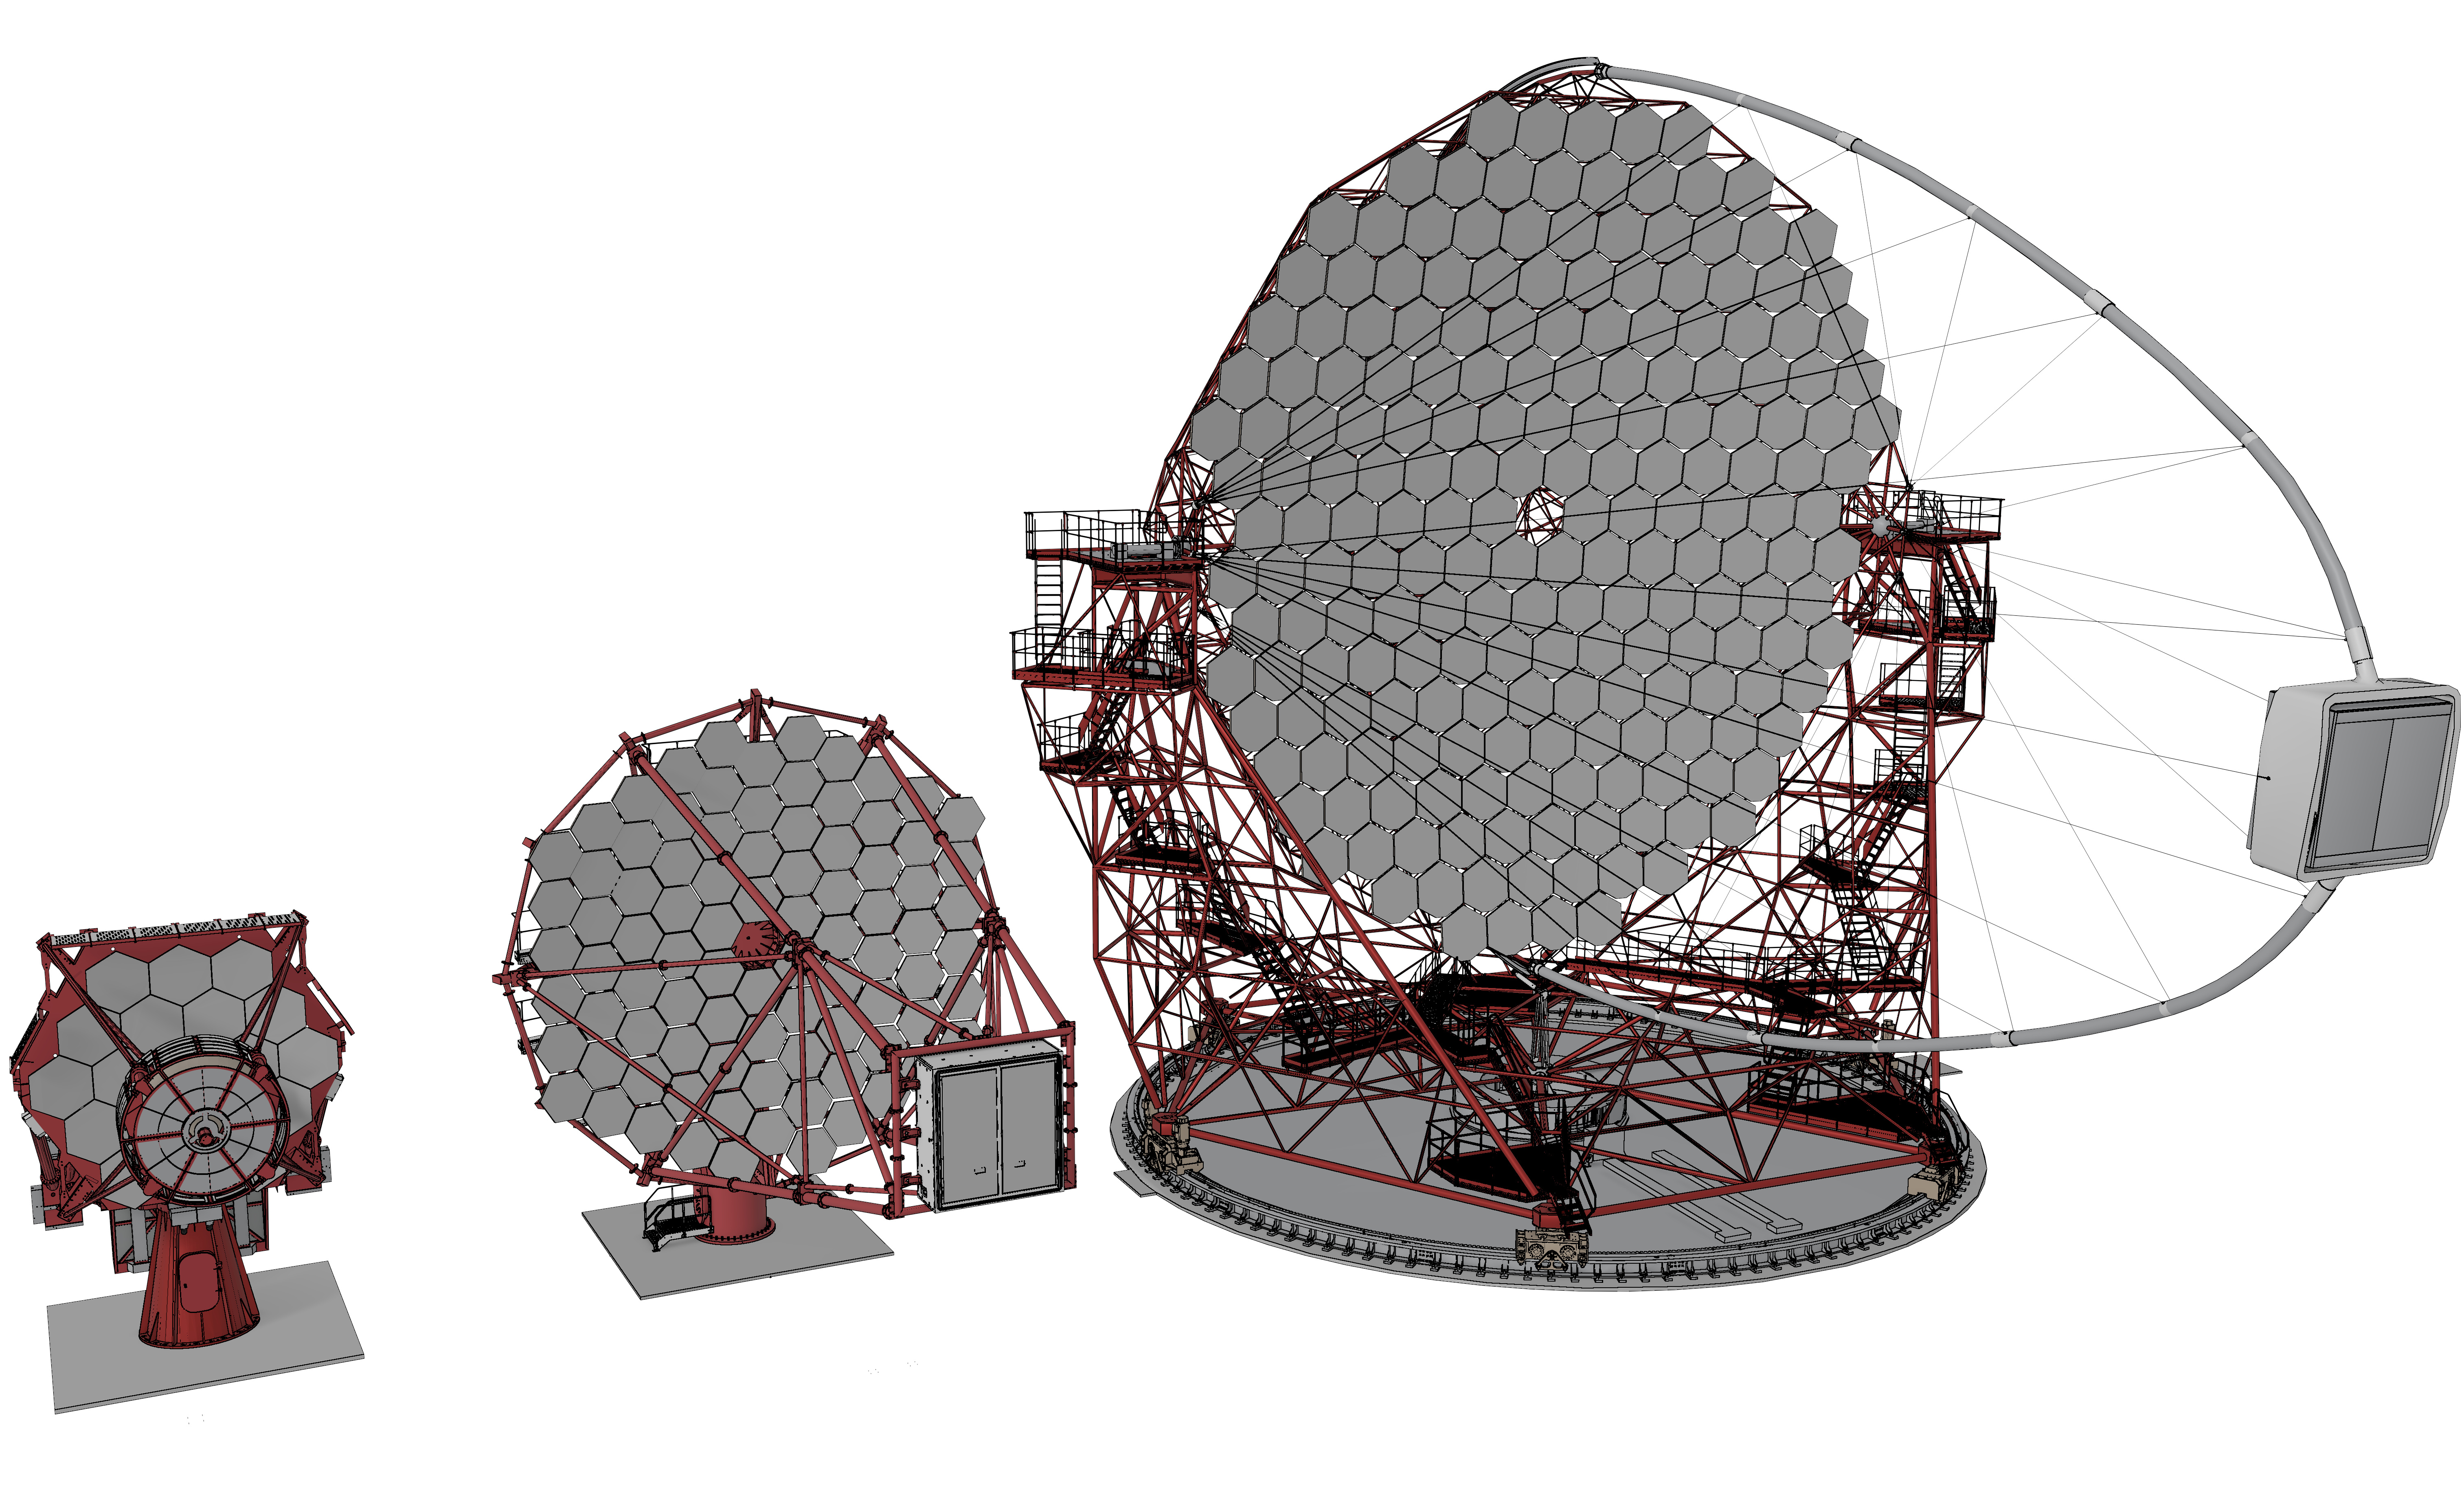
\includegraphics[width=\textwidth]{figures/composite.jpg}
  \caption[Renderings of the individual CTA telescopes]{Renderings of an LST, SST, and MST telescope.
  The LST on the right side has about four times the mirror area of the MST on the left. 
  A prototype of the MST structure was built in Berlin Adlershof where it currently undergoes mechanical testing. 
  Of the three SST prototypes, the ASTRI model will most likely be the one deployed for CTA. 
  The ASTRI telescope is a two-mirror design that allows for a very wide field of view without introducing strong aberration effects.
  All telescopes use active-mirror-control technology that continuously adjusts each individual mirror facet. This helps to compensate 
  for the deformation of the telescope's structure while sources in the sky are being tracked. 
  The LST structure is mounted on bogies running on a flat track of rail with a diameter of approximately \SI{24}{\metre}.
  It weighs a total of 103 tons, of which the camera alone makes up just under 2 tons~\cite{lst_design}. 
  Its slender-looking design is made possible by the use of carbon fiber composite materials.
  This image was rendered using Blender 2.8~\cite{blender} with models provided by G. Pérez Diaz of the Instituto de Astrofísica de Canarias.}
  \label{fig:tel_renders}
\end{figure}


\chapter{Processing CTA Data }
\label{ch:cta_analysis}

The physics performance of the CTA project can only be gauged from simulated data. 
Simulations for Cherenkov telescopes as described in \cref{sec:irf} 
track single particles and their secondary products through the atmosphere. Each single Cherenkov photon produced in an air shower 
is propagated to the virtual camera using ray tracing.
For a project as large as CTA, with its vast collection area on the ground, this becomes especially challenging. 
The distribution of Cherenkov photons on the ground are too large to store on disk. Instead, the data is piped directly into the
simulation of the telescope's optics and electronics. With a total of 99 telescopes on the ground at the Paranal site, this takes up large 
parts of the entire CTA computing infrastructure. 
Air-shower simulations for CTA, as for every IACT, are performed by the \corsika software~\cite{corsika}. The detector simulation is computed
by a program called \simtel. This software is maintained by Konrad Bernlöhr and was previously used to simulate 
data for the \hegra and \hess telescopes~\cite{simtel}.
So far, CTA data for the final layouts only exists in simulated form. However, the development of analysis software already is well underway.
The result of the simulations resemble the data from real telescopes as much as possible. The simulated data essentially produces 
uncalibrated raw data. The task of the data processing for CTA is to read the raw data and reconstruct 
information about the primary particles for each air shower.  
Early CTA analysis was performed by the \eventdisplay~\cite{eventdisplay} and \mars~\cite{magic_mars} programs.
These \rootcern and \cpp based projects have originally been developed for the \veritas and \magic 
projects. Both packages are proprietary to their respective collaborations and were used in the early stages of CTA's development.
The new software, \ctapipe, is a \python project developed under open-source licenses. 
The intention behind the design of \ctapipe is to create a fully configurable analysis pipeline for all CTA telescopes that adheres to all 
provenance requirements set by the CTA consortium. 
As of now, \ctapipe can perform preprocessing of simulated data, noise removal, extraction of image features, 
and reconstruction of the air shower's direction, as I will describe in the coming sections. 
\Cref{sec:pipeline} gives details about the \ctapipe-based preprocessing pipeline and the datasets used throughout the next chapters.
Details on the feature extraction methods, the so-called Hillas analysis, are given in \cref{sec:hillas}.\index{Hillas}
\Cref{sec:direction} elaborates on the direction reconstruction implementation in \ctapipe.
Both background suppression and energy estimation are performed by machine-learning methods which will be the topic of \cref{ch:ml}.


\section{Preprocessing Pipeline and Simulated Datasets}
\label{sec:pipeline}
The \ctapipe project in version 0.6.2 does not yet provide a fully featured and configurable application 
to process simulated raw data. 
While \ctapipe comes with basic tools to build configurable command line applications, this part of the code was only recently overhauled 
and is still in an early test phase. In \ctapipe a \emph{container} metaphor is used to encapsulate data. 
Rudimentary support for input and output of these container types is already available.
Using these features for large productions is, unfortunately, still problematic at this point. 
This is mostly due to the fact that no common file standards and formats have been agreed on in the CTA collaboration. 
The \ctapipe preprocessing pipeline reduces the raw data to a tabular structure which can be used to train 
machine-learning models for energy estimation and background suppression.
This tabular structure is called data level 2 (DL2) in the CTA vernacular.
The predictions of the trained models are then appended as new columns to the rest of the DL2 data.
Consequently, one of the requirements for a DL2 storage format is the capability to efficiently add, select, and remove columns. 
The DL2 data is also the input for the computation of the instrument response functions as described previously in \cref{sec:irf}, and therefore 
has to contain meta information about the air-shower simulations. 
The search for an official DL2 data format comes down to a tradeoff between columnar and row-wise storage.
In machine-learning use cases, the data is often queried and operated on in a column-wise manner.
Hence, a storage format is preferable that only reads the selected columns into memory. 
On the other hand, the processing of raw data happens event-wise. Therefore, appending rows to existing files has to be as efficient as possible.
The file standard currently under consideration for CTA is \hdf, which supports both storage modes. 
The \hdf standard provides hierarchical binary storage with built-in compression capabilities~\cite{hdf5}. 
The \ctapipe solution writes its data in row-wise form. This might proof to be useful in the future once data 
needs to be written under real-time constraints. 
For the analysis of simulated data, however, the runtime performance of the append operation is of lesser importance. 
For my use case, analysis of simulated data, I chose column-wise storage which allows for memory-efficient machine learning 
on a typical desktop computer. 
This format allows me to store single telescope information, array-wide event information and simulation settings within a single file.
I use the methods implemented in \ctapipe to build a custom preprocessing pipeline which can be configured using \yaml~\cite{yaml} files. 
The code and example configurations for the preprocessing pipeline can be found online at 
\githubcenter{tudo-astroparticlephysics/cta_preprocessing}
The list below gives an overview of the steps performed by the pipeline.
\begin{description}[style=nextline, leftmargin=0em, parsep=0.1em, itemsep=0.2em, labelindent=0em]
    \item[Raw Data Calibration] Sensor artifacts and electronic noise is removed from the raw voltage curves with the help of calibration data.
    In the simulated data only a rudimentary calibration is performed.
    \item[Integration] The calibrated voltage curves are integrated below their peak to find the estimated number of photons that hit the camera's pixel. The location of the peak 
    is used as an estimator for the mean arrival time of the Cherenkov photons. 
    \item[Image Cleaning] The group of pixels which have been hit by Cherenkov light are retained, while others are discarded. An example 
    of applied image cleaning can be seen in \cref{fig:preprocess}. 
    \item[Image Parametrization] The cleaned image is reduced to a list of descriptive features based on the shape of the Hillas ellipse as described in \cref{sec:hillas}. 
    \item[Shower Reconstruction] The point of origin and trajectory of the shower are reconstructed by using images from multiple 
    telescopes at once. \Cref{sec:direction} explains how this stereoscopic information is used by the implemented algorithms.
    \item[Output] The final results of the pipeline are written to disk. The final output contains telescope-wise as well as event-wise information.
    In order to support the computation of instrument responses, meta data about the simulation settings are stored per simulation run.  
\end{description}

CTA's air-shower simulations are performed by the \corsika software.
Its development has been ongoing since the late 1980s and was originally designed to simulate hadronic interactions in the atmosphere 
above the \kascade cosmic-ray experiment in Karlsruhe~\cite{kascade-data}. 
The propagation of the Cherenkov photons to the ground is usually performed  with the \mbox{IACT/ATMO} extension to \corsika. The extension follows the 
production of charged particles in the atmosphere and calculates the emitted Cherenkov light in each track segment.
The extension was mainly written by Konrad Bernlöhr and is still maintained by him. 
CTA's detector simulation is performed by the \simtel~\cite{simtel} program. The history of \simtel started with the \hegra array and is still used today by 
the \hess telescopes. The crucial part of any detector simulation is the realistic behavior of the telescope's trigger. 
A biased simulation will lead to instrument response functions which do not correspond to the actual behavior of the telescope.
In particular the calculation of the effective area, as seen in \cref{sec:irf}, is sensitive to errors in the simulations. 
The detector simulation uses the trajectory of each single Cherenkov photon as computed by \corsika and traces their path through the 
optical components of the telescope such as mirrors and light-guides. Once the photons have been ray traced to the virtual camera pixel, 
the detector's sensor electronics are simulated. Additionally, potential background light sources such as scattered light in the atmosphere 
have to be taken into account. Then the trigger logic is applied and the data from the \corsika is either written to disk or discarded.
This is the point in the analysis that takes up a majority of the computing time.
The calculation of the shower propagation is a slow process and most of the simulated showers are discarded. 
Research is ongoing into adapting \corsika by allowing it to stop early in the propagation process~\cite{baack}. 
These approaches try to predict whether the telescope's trigger logic will discard the shower or not.
Both \corsika and \simtel are long-running software projects with decades of history. 
Large parts of these legacy code bases have become unmaintainable and derelict over the recent years.
Efforts are ongoing to modernize both projects by rewriting or replacing them. 
The roadmap to a new and modern air-shower simulation software has already been formalized in the \corsika 8
white paper \cite{corsika8}.

To gauge CTA's physics performance on observed data, both signal and background data has to be simulated.
Large amounts of showers have to be simulated to test the preprocessing pipeline and benchmark the quality of the reconstruction and machine-learning 
algorithms.  
As mentioned in \cref{sec:iact} the majority of triggered air showers are induced by the hadronic component, protons and heavier nuclei,  of the cosmic rays.
Another background component in the low \si{GeV} energy range comes from cosmic electrons. Both particle types are simulated separately. 
While air showers that were induced by protons can be separated from gamma-ray showers by the shape of the shower, electrons create electromagnetic cascades indistinguishable
from gamma-ray showers. 
The incoming primary particles can be instantiated in two different ways. 
Diffuse simulations scatter the origin of the primary particle on the sky. 
The protons and electrons are simulated in a diffuse manner, so that their point of origin is uniformly distributed across the field of view.
This is in contrast to point-like simulations, where the point of origin is fixed in the center of the field of view.
\Cref{tab:datasets} shows the simulated datasets together with their associated simulation settings.
These datasets will be used throughout the rest of the document.
I only consider data simulated for the southern site for the analysis. 
CTA's detector simulation places multiple virtual camera prototypes into a single telescope.
I selected the \emph{LSTCam}, \emph{NectarCam}, and \emph{DigiCam} prototype hardware for my analysis 
in accordance with previous reference analyses.


\begin{table}
    \renewcommand{\arraystretch}{1.2}
    \caption[]{Datasets used for the CTA analysis. The table below lists information about the number of simulated showers, as well as the number 
    of remaining events after the telescope's trigger simulation and preprocessing have been applied. 
    During processing events get dropped if the image cleaning does not select any pixels or the image parametrization fails for numerical reasons.
    In this dataset all telescopes point in the same direction, due south with an elevation of \SI{70}{\degree}.
    In the point-like gamma-ray simulation the virtual source is situated right in the center of the array's field of view.
    I exclusively use data from the southern array in my analysis. All \input{build/num_tel_south.txt}telescopes are participating in the trigger. 
    I selected the simulated \emph{LSTCam}, \emph{NectarCam}, and \emph{DigiCam} prototype hardware for these datasets.}
    \label{tab:datasets}
    \rowcolors{0}{white!92!black}{}
    \begin{tabularx}{\textwidth}{@{}>{\columncolor{white}[0pt][\tabcolsep]}X r r r>{\columncolor{white}[\tabcolsep][0pt]}r@{}}
    \hiderowcolors 
    \multicolumn{5}{@{}l}{\textbf{Paranal Array HB9}} \\
    \addlinespace[0.2em]
     & \textbf{Gamma} & \textbf{Diffuse Gamma} & \textbf{Proton}  & \textbf{Electron} \\
     \showrowcolors 
    \input{build/dataset_info.txt}
    \end{tabularx}
  \end{table}



\section{Raw Data Processing}
\label{sec:raw_processing}

The data recorded by imaging Cherenkov telescopes is contaminated with noise and sensor artifacts. 
Some of that noise originates in background light due to stars or other diffuse light hitting the mirror.
Other noise is produced by the sensor itself or by the camera electronics. 
The raw data from the pixel sensors, be it silicon based photo-multipliers or traditional photo-multiplier tubes, 
consists of a series of voltages over time.
Data from the sensors is only transferred when a group of pixels in the camera reaches a certain voltage threshold.
In addition to these single telescope triggers, CTA uses a stereoscopic trigger system. 
Only when two or more telescopes have triggered coincidently, the data will be stored permanently. 
The collection of telescope data corresponding to one coincident trigger is called an \emph{array-event} throughout this chapter.
The part of an array-event belonging to one distinct telescope is called a \emph{telescope-event}. 
Converting the time series of voltages in each pixel to images is the first step of the \ctapipe pipeline.
This step is sometimes called signal, or image, extraction.

For the standard CTA analysis, two numbers are extracted per pixel from the voltage curves. 
The number of recorded photons
are estimated by integrating over the length of an adaptively selected time window. The result is then multiplied by the gain factor of the corresponding pixel which is 
known from calibration measurements. 
The mean arrival time of photons per pixel is estimated by finding the rising edge of the signal.
Smoothing methods are usually applied to reduce the influence of electronic noise in the signal.
This step is highly dependent on the sensor technology and circuitry used in the camera. 
The observed data will have to be carefully calibrated to compensate for any environmental effects like temperature and humidity.
CTA simulations make the rather optimistic assumption that all telescope are well cross-calibrated. 


% The time series of voltages are converted into 
The resulting images still contain noise due to background light. Only those pixels which have been hit by Cherenkov light are of consequence for the analysis. Others are discarded.
At first, pixels above a certain threshold are selected as \emph{core} pixels.
In a second pass adjacent pixels above a second, lower, threshold are selected. This process is known as \emph{tail-cut} cleaning. 
The set of selected pixels create an optical image of the air shower. 
These selected pixels can then be used to extract the geometrical properties of the air shower.
The cleaning is a crucial step in the analysis. There is a trade-off between the goal to retain as many 
Cherenkov photons from the air shower as possible while discarding noisy pixels which can bias the  
reconstruction of the shower's properties.
The cleaning levels chosen for the preprocessing are listed in \cref{tab:cleaning}

\begin{table}
    \renewcommand{\arraystretch}{1.2}
    \caption[]{Cleaning levels used for the CTA analysis.
    I selected the simulated LSTCam, NectarCam, and DigiCam prototype hardware for the datasets.
    In the first sweep the tail-cut cleaning method selects all pixels above the \enquote{core threshold}. In the second step,  
    all pixels are added whose light content is above the \enquote{neighbor threshold} 
    and which have at least \enquote{min pixels} neighboring pixels that were selected in the first step.}
    \label{tab:cleaning}
    \centering
    % \rowcolors{0}{}{white!92!black}
    \begin{tabular}{l r r r}
        \input{build/cleaning_info.txt}
    \end{tabular}
\end{table}


\Cref{fig:preprocess} shows a simulated gamma-ray event as seen by an LST type telescope. 
The left side shows the voltage curve of a single pixel which is part of the air-shower image as can be seen in the right image. The right side shows 
each pixel of the camera with the estimated number of photons on the color axis. The pixels selected by the tail-cut method are marked by the red outline.
This part of the analysis process is clearly the most data intensive task as it needs to process the lowest level of data from many
telescopes at once. 

\begin{figure}
    \centering
    \includegraphics{build/preprocessing.pdf}
    \caption[Preprocessing of CTA data]{A simulated air shower induced by a gamma ray as seen by one of the four LST cameras to be build
    at the Paranal observatory. 
    The left side of the image shows the voltage curve for a single pixel. The selected pixel lies on the edge of the 
    shower and is marked by a red edge in the right image. The right-hand side depicts the 
    image in the LST camera that shows the estimated number of photons on the color axis.
    The contour around the brightest pixels shows the group of pixels $C$ that have been selected by the tail-cut cleaning method.
    This gamma ray was simulated with an energy of \input{build/preprocessing_energy.txt} and triggered a total of \input{build/preprocessing_multi.txt}
    telescopes in the array. 
    }
    \label{fig:preprocess}
\end{figure}


\section{Image Feature Extraction}
\label{sec:hillas}
\newcommand{\imagerot}{\psi}
Properties of the incoming primary particle can only be inferred from the air-shower's Cherenkov emission. 
The classical IACT analysis uses the pixels selected by the cleaning step to calculate the so-called Hillas-parameters\index{Hillas}
which describe the shape of the Cherenkov emission.
In his seminal conference proceeding for the International Cosmic-Ray Conference 1985, Michael Hillas~\cite{hillas} used air-shower simulations for the \whipple telescope to find parameters which allow for the
separation between air showers from gamma rays from those started by cosmic rays. This early work is noteworthy due to the fact that it led to the first 
observation of a \si{TeV} gamma-ray source, the Crab Nebula, and started the success story of IACT technology.
Hillas proposed to approximate the shape of the air showers by an ellipse and use its geometric parameters for further analysis.
In particular the \emph{width} and \emph{length} of the observed ellipse serve as a discriminating feature.  
They describe the standard deviation of the Cherenkov photon distribution along the major and minor axis of the ellipse.  
Early papers described the calculation 
of the parameters by using rather complex equations gained from analytical least-squares fitting 
of the ellipse's major axis and then rotating the coordinates before calculating the standard deviations 
along the axes. One example can be found in appendix of the 
paper describing the first successful observation of the Crab Nebula by the \whipple telescope~\cite{whipple_crab}.
A simpler, and quicker, calculation of the Hillas ellipse can be performed by diagonalizing the covariance matrix of the photon distribution.
Let $p = (X, Y)^T$ be a two-dimensional vector of random variables $X$ and $Y$ describing the position of the Cherenkov photons on the camera. 
Then their covariance matrix is defined as
\begin{equation*}
    \mathbf{V_{\mathbf{p}}} = \begin{pmatrix}
                                \operatorname{Var}(X)   & \operatorname{cov}(X, Y) \\
                                \operatorname{cov}(X, Y)& \operatorname{Var}(X)
                            \end{pmatrix}.
\end{equation*}
% Covariance matrices are, by definition, positive semi-definite and hence all of its eigenvalues will be positive as well.
The decomposition of the covariance matrix of $p$ yields a set of orthogonal eigenvectors.
The vector associated with the largest eigenvalue points into the direction of largest variance i.e the major axis of the Hillas ellipse. \index{Hillas}
The eigenvalues are the variances of the distributions along these directions.
Hence, the Hillas \emph{width} and \emph{length} are then simply calculated as the square root of the eigenvalues.   
% These vectors are often called the principal components of the covariance matrix.
This process is also known as \emph{Principal Component Analysis}.

The true distribution of Cherenkov photons $p$ can be approximated from the cleaned camera image.
Each pixel in the camera collects the photons in the area defined by its entry window. 
If the tail-cut cleaning selects the pixels which mostly contain Cherenkov photons, 
the resulting camera image can be interpreted as a binned measurement of the true photon distribution. 
The values in the cleaned image correspond to frequency weights. 
Given camera pixels of equal area, the covariance matrix for $p$ can be calculated by the weighted variance of the selected pixel set $C$
\begin{equation*}
    \operatorname{Var}(X) \approx \frac{1}{W} \sum_{c \in C} w_c (x_c - \bar{x}_w)^2,
\end{equation*}
where $\bar{x}_w$ is the weighted mean $x$-position, $w_c$ is the weight of pixel $c$, and $W$ is the sum of all weights in $C$.
The weighted covariance is defined accordingly
\begin{equation*}
    \operatorname{Cov}(X) \approx \frac{1}{W} \sum_{c \in C} w_c (x_c - \bar{x}_w) (y_c - \bar{y}_w).
\end{equation*}
The mean coordinate of the shower, $(\bar{x}_w, \bar{y}_w)$, is often called the center of gravity (cog)
\begin{equation*}
    p_{\text{cog}} = \frac{1}{W} \sum_{c \in C} w_c \begin{pmatrix}
        x_c \\
        y_c
    \end{pmatrix}
\end{equation*}
and describes the mean of the photon distribution.
The angle $\imagerot$ defines the orientation of the major axis with respect to the horizontal axis of the camera.
It is calculated from the first and second component of the covariance matrix's eigenvector $\mathbf{v}$ with the largest eigenvalue 
\begin{equation*}
    \imagerot = \operatorname{arctan}\left( \frac{\mathbf{v}_y}{\mathbf{v}_x} \right).
\end{equation*}
Note that the ambiguous definition of $\operatorname{arctan}$ is used here instead of $\operatorname{arctan2}$, as no preferred direction is defined 
for the ellipse itself. 
The sum of weights $W$ encodes another important property of the shower which is often called \emph{size} or \emph{intensity}.
It is a proxy for the air shower's total brightness in terms of emitted Cherenkov radiation. It correlates strongly with the primary particles initial kinetic energy. 
Higher order moments along the shower's axis can be calculated once the eigenvectors and $\imagerot$ have been calculated. The skewness of the light distribution, i.e. 
the third moment along the major axis, is an indicator for the travel direction of the shower. Similar information can be extracted from the arrival time of the photons 
in each pixel. 
Another feature is the \emph{leakage} of the image. It is defined as the number of pixels, or sum of weights of pixels, which lie on the outer edge of the camera.
This feature is useful to discard images which are not fully contained within the camera.
% Another useful feature is the \emph{concentration} of the image. It is defined as the ratio of the weight in the brightest pixels compared to all other pixels in the shower.
% Appendix~\ref{ap:features} lists all features calculated by the \ctapipe analysis.


% For the analysis a presented here 
% This is the implementation of the Hillas parameters as I implemented it for the \fact telescope. A similar \python implementation was then contributed 
% to \ctapipe by Max Nöthe. 

\newcommand{\nvec}{\mathbf{n}}
\newcommand{\hmax}{H_\text{max}}

\section{Geometrical Shower Reconstruction}
\label{sec:direction}
As explained in \cref{sec:bg_estimates}, the cosmic-ray background is isotropically distributed across the sky.
Gamma-ray sources, either extended or point-like, can be distinguished from the cosmic-ray background only when the reconstruction
of the gamma-ray direction is accurate. The better the reconstruction of the gamma ray, the higher the significance with which a 
source can be detected. 
The optical system of an IACT is focused on the upper parts of the atmosphere, where most air showers 
emit their Cherenkov light.
In general, the effective area and energy range of an IACT is limited by its field of view and its mirror size respectively.
A larger mirror helps collect more light and allows recording very dim showers. Unfortunately, 
a large mirror, and hence a large aperture, reduce the depth of field of the telescope and only parts of the shower 
are in focus.  New detector types, like the \emph{Cherenkov-Plenoscope}~\cite{sebastian}, are proposed to remedy this problem. 
Similar to a thin optical lens, aberration effects and distortions can negatively impact the image quality. 
Compared to a typical imaging telescope, the requirements for an IACTs optical system are less stringent in terms of mirror precision. 
For any digital imaging system, a point-like light source has to be mapped onto the area of 
a single pixel in the focal plane in order to produce a sharp image. As the typical pixel size for an IACTs is in the order of centimeters, 
mirror precision is less crucial.
However, since IACTs are completely exposed to the elements, their durability and stability is of much higher importance. 
In addition, these large structures which hold the mirrors and cameras of the telescope are not completely stiff. 
Each change in elevation angle requires a correction of the mirror alignment. All large IACTs use active mirror control 
to constantly align their mirrors with the camera. 
The geometric information of the shower can be reconstructed with an IACT due to the fact that its mirrors act much like a thin lens.  
The mirrors of an IACT uniquely map coordinates in the sky to coordinates in the focal plane of the telescope.
As seen in the previous section, the major axis of the Hillas ellipse points along the main axis of the air shower which in turn points along the primary particles 
trajectory. 
In the image of a single telescope, the major ellipse axis does not uniquely specify a point of origin in the sky.
In fact, the showers point of origin can lie anywhere on the line defined by the major axis. 
The reconstruction of the primary particles direction has a great impact on the telescopes sensitivity. 
% The incident primary particle might have originated anywhere along the major axis.
For a single telescope, extensive shower simulations are needed to use higher order features about the image shape to determine
the point of origin along the line of the major axis. This is known as the \emph{disp}-method among Cherenkov astronomers~\cite{domingo_disp}. 

A CTA array-event will always have the information of at least two telescopes available to describe the observed air shower.
The stereoscopic view augments the Hillas parameters with additional information about the showers shape and direction.
A simple stereoscopic reconstruction technique was introduced by the \hegra experiment~\cite{hegra}. It works by superimposing the 
images of each telescope onto a common camera coordinate system. The intersection point between each pair of major ellipse axes
is calculated and averaged to determine the point of origin on the sky.

During my research stay at CEA Paris, I adapted the \hegra methods for implementation in \ctapipe. 
Previous implementations in \ctapipe used numerical minimization algorithms to find the point of intersection. In my implementation the 
intersection is found by linear least-squares methods.
In contrast to \hegra, CTA consists of telescopes with different focal lengths. The combination of different telescope sizes requires the transformation to 
a common coordinate frame relative to the local horizon.
The coordinate frames and transformations in \ctapipe were implemented by Maximilian Nöthe. They rely on \astropy's coordinate API, which allows for 
transitive transformation operations between coordinate frames.
The definition of the altitude and azimuth angles in \ctapipe follows \astropy's conventions in which an azimuth angle of \SI{0}{\degree} points due north and  
\SI{90}{\degree} points east. An altitude angle of \SI{0}{\degree} points parallel to the ground. 
The telescopes in the simulated datasets all point in the same directions with an altitude angle of \SI{70}{\degree} and 
an azimuth of \SI{180}{\degree}.
Given the pointing direction of a telescope in the horizontal frame, every point in the telescope's camera
can be transformed into a tuple of altitude and azimuth coordinates. 
% The maximum offset to the pointing direction of the array is limited  its field of view. 
In analogy to the \hegra method, the major axis of the ellipse in each telescope is transformed into the horizontal coordinate frame. 
This is achieved by selecting two points on the major axis in the camera.
The first selected point is the center of gravity. Per definition it has to lie on the ellipse's major axis.
The second point $p_{\text{t}}$ is offset from the center of gravity by an arbitrary distance $a$ in the direction $\imagerot$ along the main axis  
\begin{equation*}
    p_{\text{t}} = p_{\text{cog}} + a \begin{pmatrix}
        \cos(\imagerot) \\
        \sin(\imagerot) 
    \end{pmatrix}.
\end{equation*}
The transformed points $p_{\text{t}}$ and $p_{\text{cog}}$ together with the telescope's position on the ground define a
\emph{plane} in the euclidean space. A plane, in mathematical terms, is given by two vectors and a point of origin. 
Each telescope participating in the triggered event defines such a plane with an accompanying 
normal vector $\nvec$. 
The intersection between two, non-parallel, planes 
is given by a line whose direction is found by taking the cross product between the planes' normal vectors.
The intersection between the planes points along the direction of the recorded air shower. 
Similar to the \hegra approach, each ordered pair of normal vectors $(\nvec_i, \nvec_j)$ is used to find an intersecting line which is then combined with a weighted sum 
\begin{equation*}
    \hat{d} = \sum_{(i, j) \in S} c_i c_j \,  (\nvec_i, \nvec_j),
\end{equation*}
where $S$ contains all combinations of indices $i$ and $j$ for which $i < j < N$. For an event with $N$ participating telescopes, $N(N - 1)$ intersections are evaluated.
In the current \ctapipe implementation (version 0.6.2) the weights are calculated as $c = W \frac{l}{w}$, where $W$ is the total intensity of the shower and $w$ and $l$
are the width and and length of the Hillas ellipse.\index{Hillas}
This simple heuristic puts emphasis on shower images that are bright and elongated for which the shower orientation $\imagerot$ can be reconstructed accurately.
\Cref{fig:ang_res_raw} shows the angular resolution of this reconstruction method for bins in simulated energy. 
The angular resolution is defined as the 68\th percentile of the distance between estimated and simulated source position and is indicated by the blue line. 
The histogram in the background shows the underlying distribution of the simulated gamma rays. 


In addition to the direction of the shower, the height of the showers maximum lateral distribution $\hmax$ can be estimated.
The $\hmax$ variable describes the point along the trajectory of the air shower at which the amount of produced secondaries starts to decrease.
This corresponds to the point in the camera image in which the Hillas ellipse has its largest extension i.e. its center of gravity.\index{Hillas}
The $\hmax$ feature correlates with the primary particles energy and type. The more energy the primary particle had, the longer the trajectory of the air shower 
before the all energy has dissipated. 
Therefore, the height above ground at which the shower was brightest can be used for energy estimation as well as background suppression. 
In \ctapipe the estimation of $\hmax$ is performed using a least-squares method.
The center of gravity $p_{\text{cog}}$ in each shower image is transformed into the local horizontal frame and then into the euclidean coordinates.
This vector $\mathbf{v}_i$ together with the telescope's position $\mathbf{v}_{\text{tel}, i}$ defines a line running from the telescope to the brightest part in the shower. 
In a second step, the closest point to a common intersection point between all $N$ lines is estimated.
Following arguments from~\cite{line_line} the point closest to all other lines can be found using matrix methods. In the first step the matrix 
$\mathbf{M}_i = \mathbf{1} - \mathbf{v}_i \mathbf{v}_i^\top$ is build for all participating telescopes in the event. 
The closest mutual point $p_{\hmax}$ to all lines is then found by calculating
\begin{equation}
    \label{eq:line-line}
    p_{\hmax} = \left(\sum_i \mathbf{M}_i \right)^{-1}  \sum_i \mathbf{M}_i \mathbf{v}_{\text{tel}, i}.
\end{equation}
\Cref{fig:hmax_raw} shows the estimated $\hmax$ for simulated diffuse gamma rays together with the true height.
While the estimator is clearly biased and systematically underestimates the true $\hmax$,
the trend of decreasing $\hmax$ with increasing energy is followed. Hence, it can be used as a useful feature for training the energy estimator.

Another important shower parameter is the impact point of the shower trajectory on the ground. It is calculated using the lines defined 
by the reconstructed major axis of the shower in each camera. As before the closest mutual point, the closest point to a common intersection, can be found using the 
least square solution from \cref{eq:line-line}. The distance of each telescope to the impact point is another helpful feature for energy estimation. 
Showers which trigger the camera despite large distances, have to emit a lot of light and therefore have a large energy content. 


\begin{figure}
    \centering
    \includegraphics{build/ang_res_raw.pdf}
    \caption[Angular resolution for diffuse gamma rays]{Angular resolution for diffuse gamma rays.
    The blue line shows the 68\th percentile of the distance between estimated and simulated source position in each energy bin. 
    The hexagonal histogram in the background shows the event distribution. 
    From the minimum energy up to approximately \SI{2}{TeV} the angular resolution improves. This is expected behavior as the reconstruction of the major axis orientation $\imagerot$ improves with increasing 
    image brightness. At even higher gamma-ray energy the shower images are often not fully contained within the telescope's field of view and 
    cannot be reconstructed properly. The distribution of events is clearly skewed towards large distances. The peak of the distribution 
    is located near \SI{0.1}{\degree}. For most events, the direction is reconstructed accurately. Many of these outliers would be removed for the actual 
    analysis, whose event selection is optimized for a specific use case. An example will be shown in \cref{ch:sensi}. 
    It is important to note that the distance is calculated between points given in a horizontal coordinate frame which is spherical.
    The distance between two points on a sphere can be calculated using the Vincenty formula~\cite{vincenty}. For this plot, and similar plots following 
    in the coming sections, the \astropy implementation of spherical distance computation is used.
    The dataset shown in the figure contains \input{build/gamma_test_num_array_events.txt} array-events with a total of \input{build/gamma_test_num_tel_events.txt} 
    single telescope-events.
    }
    \label{fig:ang_res_raw}
\end{figure}

\begin{figure}
    \centering
    \includegraphics{build/hmax_raw.pdf}
    \caption[Max height reconstruction accuracy.]{The blue line shows the estimated height above ground at which the lateral distribution of Cherenkov photons is the largest. 
    The shaded blue area indicates the 16\th and 84\th percentile of the estimation.
    The distribution in the background shows the simulated $\hmax$ values. The horizontal lines in the $\hmax$ distribution are due to binning effects 
    in CTA's air-shower simulation.  The estimator follows the same shape as the $\hmax$ 
    distribution, making it a good feature for energy estimation and background suppression.
    }
    \label{fig:hmax_raw}
\end{figure}
% \begin{figure}
%     \centering
%     \includegraphics{build/ang_res_raw_mult.pdf}
%     \caption[]{Angular resolution for diffuse gamma-rays for different event multiplicities.
%     The colored lines show the 68\th percentile of the distance between estimated and simulated source position in each energy bin. 
%     Unsurprisingly, a higher number of triggered telescopes yields a more accurate directional reconstruction since more stereoscopic information 
%     is available.
%     }
%     \label{fig:ang_res_raw_mult}
% \end{figure}
\begin{figure}
    \centering
    \includegraphics{build/impact_distance_raw.pdf}
    \caption[Reconstruction of the impact distance]{The two-dimensional histogram shows the distribution of the distance between the true impact position and 
    the estimated impact position of the shower on the ground for bins in simulated energy.
    The blue lines indicate the median of the distribution in each bin.
    }
    \label{fig:impact_distance_raw}
\end{figure}

% The center of gravity
% CTA software used expensive numerical minimization algorithms in order to reconstruct the shower's impact position on the ground.
% I was able to express the problem as a linear optimization problem which simplifies the problem to simple matrix calculations and least-squares methods.
% This greatly reduced both runtime and complexity of the method without reducing the accuracy of the reconstruction.

% In my thesis I test the performance of the geometric reconstruction in terms of angular resolution and runtime. The
% new algorithms have been included in CTA's official preprocessing pipeline.

\newcommand{\mbf}[1]{\mathbf{#1}}
\newcommand{\yhat}{\hat{y}}
\newcommand{\ghat}{\hat{g}}
\newcommand{\data}{\mathbf{X}}
\newcommand{\truth}{\mathbf{y}}
\newcommand{\traindata}{\mathbf{X}_{\text{train}}}
\newcommand{\testdata}{\mathbf{X}_{\text{test}}}
\newcommand{\trainlabel}{\mathbf{y}_{\text{train}}}
\newcommand{\testlabel}{\mathbf{y}_{\text{test}}}
\newcommand{\column}{\mathbf{x}}
\newcommand{\prediction}{\hat{\mathbf{{y}}}}
\chapter{Machine Learning}
\label{ch:ml}
Machine learning for this CTA analysis is used for energy estimation of the primary gamma ray and background suppression.
As mentioned in \cref{sec:iact}, cosmic-ray showers, i.e. hadronic showers, build the main 
background component in IACT data. A model which can separate air-showers induced by gamma rays from those started by hadrons,
boosts the detection significance of an IACT considerably. 
Energy estimation is necessary to learn about a sources energy spectrum and the acceleration mechanisms taking place in it.
From simulated data, where the true values for the particles type and energy are available, a model can be built 
which takes image parameters as input and predicts the output values on new, unlabeled, observations. 

In the early days of IACT analysis, these model functions weere often hand-crafted.
For background suppression a set of \emph{cuts} were defined in the image parameter space. 
By looking at the distribution of the hillas parameters for simulated gamma rays and protons, the location of a cut can be 
fixed and then applied to observed data. 
The \hegra analysis from 2004~\cite{hegra-crab-data}, for example, used a simple cut in the width of the Hillas ellipse to reduce the 
amount of background events in their data. 
Energy estimation for \hegra used a similar approach. Correlation plots between image parameters and true energy were used 
to find the shape of analytical function whose parameters $\mathbf{p}$ were fitted.
These approaches are flawed. The choice of parameters in which to place the cuts and the choice of analytical functions for energy 
estimation is utterly subjective. Not to mention the fact that the capacity of human brains to work in many dimensions is limited.
These shortcomings can be overcome by supervised machine-learning algorithms.

Here I mostly follow the notations and definitions from the book \enquote{Elements of statistical Learning} by Trevor Hastie and others~\cite{hasties}.
Given a set of $N$ observations with $p$ variables the matrix $\data$ 
contains the full information needed to train a machine-learning model. In this so-called \emph{data matrix}
each column corresponds to an observed variable. Each row maps to a specific observation.
The columns in $\data$ are called differently depending on context and personal preference. 
Common choices are observables, variables or features. 
One specific observation $x \in \data$ is written as a small letter. 
The $j$\th entry, or feature, in one observation is indexed by $x^{(j)}$.
In a similar manner,
a single uppercase letter such as $X$ denotes a generic random variable.
The $i$\th observed value of $X$ is written as $x_i$. 
Vectors containing entries for each of the $N$ observations are set in bold lowercase $\column$.
In this specific use case, the columns in $\data$ map to the image parameters and the rows to the observed air showers. 
If $X_{w}$ is the random variable describing underlying the distribution of observed Hillas widths, then
$x^{(w)}_{i}$ is the Hillas width from one observed air shower in one telescope and $\mbf{x}^{(w)}$ is the vector containing all observed Hillas widths.
For the each observation we also have an associated \emph{output} or \emph{truth} $y$ stored in the vector $\truth$.
The true label values in the CTA simulations come in two distinct forms. 
The energy of a particle $y \in \mathbb{R}$ is a continuous parameter, 
whereas the type of the particle is a discrete variable that can take only one of two values $g \in \{\text{gamma}, \text{hadron}\}$.
The labels values are encoded as numbers by convention so that $g \in \{0, 1\}$.
For the sake of simplicity I do not always differentiate between the continuous $y$ and the categorical $g$ in some of the following definitions.
Roughly following the definition in~\cite[10]{hasties} we can now specify the task of supervised machine learning as follows:
\begin{quote}
    Given a $N \times p$ matrix $\data$ and some associated output vector $\truth \in \mathbb{R}^N$,
    find the function $f(\data) = \prediction$ that takes a vector $\data \in \mathbb{R}^p$ and returns a prediction for $\truth$
    and minimizes some \enquote{loss function} $L(\truth, f(\data))$ over the data and the true label. 
\end{quote}
If $\truth$ is continuous, then $f$ is called a \emph{regressor}. If $\truth$ is categorical, then $f$ is called a \emph{classifier}.
In this formulation supervised machine learning can be understood as a global optimization problem. 
The space of possible solutions has to be constrained to find valid solutions with any predictive power.
Usually, the shape of the function $f$ is fixed for a machine-learning algorithm. It is parameterized in some form by a vector $\beta$ 
whose entries are found by minimization with respect to the loss. This step is often called \emph{training} the 
classifier or regressor.

The textbook example for a choice of $f$ and $L$ is the least-squares regressor~\cite[11]{hasties} which exemplifies some of the important properties 
of supervised machine-learning methods.
Assuming $f$ is a linear function in the data $\data$ then it can be written as 
\begin{equation*}
    f(\data; \beta) = \prediction =  \beta_0 + \sum_{j=1}^p \column^{(j)} \beta_j.
\end{equation*}
The loss function for the least-squares method is the residual sum of squares which can be written as
\begin{equation*}
    L(\truth, f(\data), \beta) = \sum_{i=1}^N (y_i - f(x_i; \beta))^2 = \sum_{i=1}^N (y_i - x_i \beta)^2,
\end{equation*}
where the data matrix was implicitly modified to contain series of ones $(1, 1,...,1)$ as the first column and $\beta$ is a column vector $\beta=(\beta_0, \beta_1, \ldots, \beta_p)^\top$.
From this expression an analytical solution for $\hat{\beta} = \argmin_{\beta} L(\truth, f(\data), \beta)$
can be found by setting the derivative with respect to $\beta$ equals zero
\begin{align*}
    \dddp{L}{\beta} \stackrel{!}{=} 0 &= \ddp{\beta} \sum_{i=1}^N (y_i - x_i \beta)^2 \\
                                      &=  -2 \cdot \sum_{i=1}^N x_i (y_i - x_i \beta)  \\
                                      &=  2 \cdot {\data}^{\top} (\truth - \data \beta).
\end{align*}
Solving for $\beta$ yields 
\begin{equation*}
    \hat{\beta} = ({\data}^\top \data)^{-1} {\data}^\top \truth.
\end{equation*}
% The regressor can now predict the value of $\yhat$ 
The linear least-squares method essentially fits in hyperplane in the parameter space spanned by the provided data and true label $y$.
If the values of $\truth$ are continuous, then $\prediction = f(\data; \hat{\beta})$ is the result of the regressor and can be used as is.
In the case of classification, the fitted hyperplane, or the function $f(\data; \hat{\beta})$, can be used to define a decision boundary or threshold $\alpha$. 
The classification function is then defined as 
\begin{equation*}
    \hat{g}_i = f'(x_i; \hat{\beta}) = \begin{cases}
        0, & \text{if } \; f(x_i, \hat{\beta}) < \alpha \\
        1, & \text{else.}
    \end{cases}    
\end{equation*}
In case the true label for the binary classification problem $g$ or $y$ was encoded using values $\{0, 1\}$, then 
the canonical value for the threshold is  $\alpha = 0.5$.
The decision boundary is hence defined by all points where $f(\data; \hat{\beta}) = 0.5$.
Intuitively speaking, new observations are classified based on their location relative to the fitted hyperplane. 
The distance of a new observation to the decision boundary can be understood as a measure of \enquote{certainty} of the point belonging to either class. 
\Cref{fig:boundary} shows an artificial dataset on which a least-square regressor was trained. 
The points in the figure are colored to indicate the class to which they belong. 
It is also obvious from the figure that the raw output of the least-square regressor is not a proper probability density as it is neither bounded nor normalized. 
This makes the interpretation of the regressors output difficult to interpret.
It can, however, be transformed into a value range resembling a probability density by wrapping the output of 
the least-squares predictor in a so-called sigmoid function $S(f(\data; \hat{\beta}))$
\begin{wrapfigure}{o}{0.5\linewidth}
    \centering
    \includegraphics{build/boundary.pdf}
    \caption[Least squares machine learning example]{The transparent plane in the figure shows the result of a least-squares fit to the data.
    }
    \label{fig:boundary}
\end{wrapfigure}
The family of sigmoid functions is loosely defined by their properties to be 
monotonically increasing and bounded by horizontal asymptotes %, i.e. $S(m_1) \leq S(m_2)$ if $m_1 < m_2$,
for $m \rightarrow \pm \infty$.
The error function shown in \cref{fig:erf} is an example of a sigmoid function.
If the sigmoid function is bounded by 0 and 1,
the output of $S(f(x_i; \hat{\beta}))$ can be interpreted as a probability density.
Note that this is different from a \emph{confidence level} for the prediction.
Adjusting the classifier output to resemble a confidence is the topic of \enquote{classifier calibration}~\cite{calibration1, calibration2}.
Like the least-squares approach, most classification algorithms provide a continuous output which is either bounded or can be wrapped 
by a sigmoid function.
The adaption of the decision threshold $\alpha$ is a key component in the analysis of IACT data.
As explained in \cref{sec:bg_estimates}, IACT data is heavily contaminated by cosmic-ray background. 
By increasing the prediction threshold the amount of background events can be reduced. This naturally comes with an 
inevitable decrease in selected signal events. The choice of $\alpha$ is optimized for different physics use cases.
In \cref{ch:sensi} the prediction threshold will be optimized for the detection of gamma-ray point sources. 
The correct way to validate one's classification model is often hotly debated within physics research groups.
The validation methods I use for the CTA analysis are described in \cref{sec:validation}.
\Cref{sec:trees} explains the basics of decision tree algorithms on which both the background suppression and energy estimation are based. 
Results of the training and the application of the models to CTA data is shown in \cref{sec:results}.
\Cref{sec:aict} describes the software we developed to create a reproducible machine-learning pipeline for the CTA and \fact telescopes. 


\section{Model Validation}
\label{sec:validation}
Models for classification or regression can only be properly evaluated on labeled data.
Some machine-learning algorithms tend to \emph{overfit} on the training data. 
While the models minimize the loss $L$ on the training data to a great extend, it does not generalize well to new data.
In other words, it has weak predictive power on hold-out data.
In literature this problem is known as bias-variance tradeoff, overtraining, or \emph{overfitting}.
A model fitted on some training data $\traindata$ with label $\trainlabel$ needs to be applied to an independent dataset $\testdata$
that comes with an associated label $\testlabel$ in order to get an estimate of it generalization capabilities.

A classifier's performance in terms of predictive power is estimated from its \emph{confusion matrix}.   
In a classification problem with two categories, like the distinction of gamma-ray air showers from hadronic ones, 
the two classes are called  \enquote{positive} and \enquote{negative} per convention. 
In IACT analysis the positive class is usually understood to be the gamma-ray events.  
The result of the model validation for a binary classification problem contains four numbers.
The number of \emph{true positives} ($TP$) which are the events that have correctly been predicted to belong to the positive class, i.e. the number of correctly identified gamma rays.
The amount of \emph{false positives}, ($FP$) the events that have incorrectly been predicted to belong to the positive class, i.e. the number of hadronic events 
that have been falsely classified as gamma-ray events. The number of \emph{true negatives} ($TN$) and \emph{false negatives} ($FN$) are defined accordingly.
These four numbers, that make up the confusion matrix, completely characterize a classifier's prediction.
A myriad of scalar quantities that try to summarize the classification can be derived from the entries in the confusion matrix. 
Popular choices include the accuracy, precision, F-score, recall or true positive rate, and the false positive rate just to name a few. 
Each come with their own advantages and disadvantages. 
The extremely common \emph{accuracy} measure, for example, is defined 
as 
\begin{equation*}
    \operatorname{acc} = \frac{TP + TN}{TP + FP + TN + FN},    
\end{equation*}
i.e. the ratio of correctly identified events with respect to the entire population.
The accuracy is only useful in the case of balanced datasets where both classes are represented by an equal amount of data points.
For imbalanced datasets the accuracy alone does provide a good estimate on the classifiers \enquote{quality}.
The balanced accuracy on the other hand is defined in terms of true positive and true negative rates instead of the absolute numbers
\begin{equation*}
    \operatorname{acc_{\text{bal}}} = \frac{TPR + TNR}{2}   
\end{equation*}
and is therefore not influenced by unbalanced class ratios.
In the case of IACT analysis datasets are often imbalanced. 
The observed data contains orders of magnitude more background events than gamma-ray showers. 
The accuracy on the simulated data in itself does not help to gauge the performance of a telescope. 


A popular method for calculating performance estimates is called cross-validation. 
A $k$-fold cross validation splits the training data into $k$ independent subsets.
One of the $k$ subsets is used as a validation set for a model that is trained on the union of the remaining $k{}-{}1$ subsets.
During cross-validation the model is trained and evaluated $k$ times. 
This yields $k$  estimations of an algorithm's classification performance on a specific training dataset. 
This allows for robust error estimates on the entries in the confusion matrix. 
It does, however, increase the runtime of the model training by a factor of $k$.
The increased runtime of the training step is tolerable considering that the application of the trained model to the CTA data takes about ten times as much time.
This is due to the fact that the largest part of the datasets presented in \cref{tab:datasets} is used to estimate the point-source sensitivity of CTA which will be the topic 
of \cref{ch:sensi}. 
Only a small part of the diffuse gammas and protons is used to train the classifier and energy estimator. It is this smaller sample which is split during cross validation. 

 
For the CTA analysis I use the cross-validated receiver operating characteristic (ROC) to gauge the performance of my classification.
The ROC curve is produced by drawing the false positive rate ($FPR$) versus the true positive rate ($TPR$) 
while varying the prediction threshold $\alpha$. The $TPR$ and $FPR$ for a fixed $\alpha$ are defined as 
\begin{equation*}
        TPR_{\alpha} =  \frac{TP}{FN} \text{\quad and \quad} FPR_{\alpha} = \frac{FP}{FP + TN}
\end{equation*}
and are therefore independent of class balance. This curve is monotonically increasing towards larger values of $FPR$. 
Instead of comparing the ROC curves themselves, different classifiers trained on the same data can be compared by the area under their respective ROC curve. 
A hypothetically perfect classifier would create no false positives and classify only true positives. Hence, the ROC curve for the perfect 
has a constant value and the area under the curve (AuC) would equal one.
A classifier that only randomly selects an outcome, would create a diagonal line with an AuC of 0.5.
The ROC and the AuC are no perfect benchmarks. Their validity has long been the spotlight of discussions in the machine-learning community
There are plenty of alternative suggestions. See~\cite{roc_auc_bad} for an example.
When large datasets are available, which is the case for CTA analysis, these problems are somewhat diminished.
Within CTA, the ROC AuC is used to the classification strengths of competing methods for background suppression. 

For regression problems no confusion matrix in the classification sense can be constructed. 
Instead a matrix showing the correlation between the true label $\truth$  and the prediction $\prediction$ is created on an independent test dataset. 
A perfect regressor would only have entries on the diagonal of that matrix. To express the quality of the regression in one number, the 
coefficient of determination or $R^2$ score is often used. The $R^2$ score is calculated from the residual sum of squares $RSS = \sum_i (y_i - \yhat_i)^2$ as used for 
the least-squares loss and the variance of the target variable $\truth$.
The definition of the $R^2$ square is 
\begin{equation*}
    R^2 = 1 - \frac{RSS(\truth, \prediction)}{ N \operatorname{Var}(\truth)},
\end{equation*}
where $N$ is the number of entries in $\truth$.
It can be understood as a \emph{goodness of fit} where a value of 1 indicates a perfect match between regressor and truth. If the regressor, on average, predicts 
the mean of the target, then the $R^2$ score will have a value of 0~\cite[486]{stats_devore}. 
For IACT analysis the $R^2$ score is not sufficient to explain the quality of the energy estimation.
Equivalently to the calculation of the angular resolution, the relative difference between the predicted and true energy is calculated
for bins in estimated or true energy.
%  The result of the energy estimation for CTA is shown in \cref{sec:results}.

\section{Decision Trees and Ensemble Learning}
\label{sec:trees}
Methods like least-squares or neural networks try to find the global minimum of a loss function which was in itself defined over the entire parameter space.
Often it is not possible to find a satisfactory solution without further assumptions about the shape of the parameter space.
The idea behind decision trees is to split the parameter space into subspaces where the problem is potentially easier to solve~\cite[305]{hasties}.
% The assumption is that the true target distribution can be approximated by series of constant values.
In each of the subspaces the loss function is then optimized independent of the data in the other subspaces. 
If no satisfactory value of the loss function is found, the subspaces are split again into even smaller sub-subspaces.
Once the partitioning has finished, each subspace $R_m$ is assigned a label $c_m$. In the regression case, the mean of the true labels from the training set in $R_m$ is assigned. 
For classification, the majority class is assigned to the subspace.
The decision function returns $c_m$ for new point $x_i$ located within the region $R_m$
\begin{equation*}
    f(x) = \sum_{m=1}^{M} c_m \mathbf{1}(x \in R_m)    
\end{equation*}
where $\mathbf{1}$ is the indicator function.
Finding the optimal partition of subspaces in order to construct a decision tree is an NP-complete~\cite{dt_np_complete} problem.
Decision tree methods employ a greedy strategy to build the partition~\cite[307]{hasties}. 
The tree is build by performing recursive binary splits of the subspace.
Starting from the tree's root, the parameter space is split at a into a set of \enquote{left} and \enquote{right} partitions.
A variable $j$ and a split value $S$ are chosen which define the partition 
\begin{equation*}
    R_L(j, S) =  \{x \in \data \mid x^{(j)}  \leq S \} \text{\quad and \quad} R_R(j, S) =  \{x \in \data \mid x^{(j)}  > S \}.
\end{equation*}
The best point $S$ and variable $j$ along which to partition the space is found by iterating through all possible
splits for all columns in $\data$ and choosing the one which minimizes the loss $(j, S) = \argmin_{(j, S)}(L)$.

For classification tasks the \emph{information gain loss} is a popular choice. 
It is known under different names such as the \emph{cross-entropy} or just \emph{entropy} criterion. 
The loss for the information gain (IG) is defined as
\begin{equation*}
    L = -\operatorname{IG}(Y, R) = -\bigl(H(Y) - H(Y \mid R)\bigr).
\end{equation*}
The function $H$ is known as the information entropy 
\begin{equation*}
  H(Y) = - \sum_{g \in G} P(Y=g) \log_2{P(Y=g)}.
\end{equation*}
For the random variable describing the target distribution $Y$. The probabilities $P$ are assumed to be uniform and are simply approximated by
the class proportions. In a binary classification problem this simplifies to
\begin{equation*}
    H = -p \log_2(p) - (1-p)\log_2(1-p),
\end{equation*}
where $p = \frac{|R_L|}{|R_L| + |R_R|}$.
The conditional entropy $H(Y \mid R(j, S))$ is the entropy of $Y$ after the split has been applied.
It can be written in terms of probabilities as
\begin{equation*}
    H(Y \mid R)  =  \sum_{\mathclap{R \in \{R_L, R_R\}}} P(X \in R) H(Y | x \in R),
\end{equation*}
where $H(Y | x \in R)$ is the entropy of $Y$ for all data points $x$ in subspace $R$.
Again, the probabilities are assumed to be uniform and can be approximated by their proportions
\begin{equation*}
    H(Y \mid R)  =  \frac{|R_L|}{|R_L| + |R_R|} H(Y \mid x \in R_L)  + \frac{|R_R|}{|R_L| + |R_R|} H(Y \mid x \in R_L),
\end{equation*}
where $|R_L|$ and $|R_R|$ is the number of samples in the left and right partition respectively.
Once the best split has been found, the process continues recursively until a stopping criterion is met.
In the case of regression, where $Y$ is continuous, the process is the same. The only difference is the choice of loss function.
For most regression problems, including the energy estimation performed here, the residual sum of squares is minimized in each partition
\begin{equation*}
    L \propto \sum_{\mathclap{R \in \{R_L, R_R\}}} \operatorname{Var}(Y \mid x \in R_L).
\end{equation*}
In other words, the split $(j, S)$ which minimizes the total variance of the target in each partition is chosen.

Tree building algorithms try to find the optimal split criterion in some local region of the parameter space.
Finding the best overall split in parameter space is computationally infeasible.
This means the decision tree algorithm can run into a local optimum. 
When building a decision tree one needs to find a balance between the tree depth and its tendency to overtrain. 
In general, a decision tree whose final nodes, or leafs, contain too few samples, does not generalize well.
The number of times a certain feature has been selected for splitting during optimization carries some notion 
of \emph{feature importance}. This is a useful diagnostic tool for validating ones assumption regarding the classification.

The idea of \emph{ensemble learning} is to train several weak classifiers on different subsets of the data and
then combine them into one strong classifier by averaging their output.
This makes the decision tree method relatively robust to overfitting without 
losing much runtime since the creation of the ensemble is trivial to parallelize.
The most common way to build a decision tree ensemble  
was popularized by Breiman~\cite{breiman-bagging}.
Here the training data is split into subsets using sampling with replacement, which is also known as bootstrapping.
An additional source of randomness, or variance, was introduced by Breiman
by limiting the choice of variables $j$ in each partition to a random subset of features. 
This construction is called a \enquote{Random Forest}~\cite{breiman-rf}. 
For use in ensemble methods another layer of randomization can be applied to the tree building process. 
Instead of iterating through all possible cuts for the $n$ randomly selected features, only $n$ randomly chosen 
splits are considered. These \emph{extremely randomized trees}~\cite{extratrees} can be used in bagged ensembles
just like the original Random Forest, but with much faster training times. 

For my CTA analysis I use and ensemble of extremely randomized trees for classification of particle type and regression of energy. 


\section{AICT-Tools}
\label{sec:aict}

To ensure reproducibility for the entire machine-learning process, 
I started the open-source \python project called \aicttools. It consists of a fully configurable pipeline 
to perform the common machine-learning tasks encountered in IACT analysis. 
Given a set of input data and configuration files, it splits the data into test and training sets,
performs on the fly feature generation, trains and applies the models, and creates the numbers and charts needed to gauge the
performance of the trained models.
Each task is dealt with by a single-purpose command line application. This was a design decision made to facilitate 
the use external tools such as \make to model the data dependencies between each task.
\cref{ch:repro} contains a short discussions on the use of Makefiles to ensure reproducibility.
% Programs such Make or similar projects are helpful tools to support reproducibility. A short discussions on the use of Makefiles can be found in \cref{ap:repro}.
The classification and regression algorithms executed by the \aicttools are implemented in the \sklearn library~\cite{sklearn}.
Arbitrary \sklearn predictors can be used by the \aicttools as long as they produce continuous output. 
Everything is configured in human readable \yaml files. 

Originally build for the \fact project, I added new functionalities to the \aicttools to support the analysis of CTA data.
The goal was to make it possible to work with data on a single telescope level, i.e. the telescope-events, as well as the array-event level.
The output of the CTA preprocessing comes in the form of three tables stored within a single \hdf file.
The logical layout of this DL2 data file can be seen in \cref{tab:dl2-structure}.
This layout brings about some challenges concerning the I/O functionalities of the \aicttools.
First and foremost, the splitting of the data into training and validation sets has to take the simulation information into account.
The data belonging to a single simulation run must not be separated. 
% The \corsika settings for the triggered data needs to be available.
 Otherwise the calculation of instrument responses and event weights, 
as described later in \cref{sec:weights}, would not be possible. 
Second, in order to train models on both single telescope features as well as array-wide information, the tables need to be merged. 
The tables are joined on the primary key which consists of the unique identifiers for the run, array-event, and telescope.
The canonical way to support this kind of operation is by using the well known \pandas library~\cite{pandas}.
While the library is a powerful tool to perform operations on table-like data, it does not support memory mapping techniques or out of memory computing.
The overhead in terms of required RAM are considerable.
For the \aicttools I implemented a way to read and merge the CTA data in a chunk-wise manner.
The \aicttools work with the full PROD3B analysis as well as the simulations for the prototype
of the CHEC camera. 
The code, including example configurations, can be found at 
\githubcenter{fact-project/aict-tools}. 

% An fully reproducible analysis of published \fact data can be executed by  i 
% For my thesis I benchmarked the performance of the produced models and optimized
% them using feature generation and nested modeling approaches which have been implemented into aict

\begin{table}
    \renewcommand{\arraystretch}{1.0}
    \caption[Data structure for data level 2]{Logical structure of the DL2 data as produced by the CTA preprocessing script. All tables are stored in a single \hdf file. 
    The unique primary keys allow for merging and joining of information. This allows for a straightforward access to the simulated values for any given 
    telescope-event. The telescope-event identified by the tuple $(58, 4100, 92)$, for example, can easily be associated with the simulated energy, \enquote{mc\_energy}, of the array-event 
    $(58, 4100)$.
    For the training of machine-learning models, the array-event table is merged with the telescope-event table.
    For application of the models the data is read chunk-wise by reading the entire index into memory and then reading blocks of
    connected array-events. 
    The table below shows the first exemplary lines 
    of the diffuse simulated gamma-ray dataset described in \cref{tab:datasets}. Some column names were shortened in order to fit the table to the page.
    A full listing of column names can be found in the \aicttools configuration file in appendix~\ref{ap:config}.}
    \label{tab:dl2-structure}
    % \rowcolors{3}{white!92!black}{}
    \begin{tabular*}{\textwidth}{@{}l l l@{\extracolsep{\fill}} r r r r@{}}
    \multicolumn{6}{@{}l}{\textbf{Runs}}\\
    \addlinespace[0.2em]
    % Run ID & & & mc\ & mc\_num\_showers & mc\_shower\_reuse \\
    % \addlinespace[0.2em]
    \input{build/dl2_info_runs.txt}\\
    \multicolumn{6}{c}{$\vdots$}\\
    \multicolumn{6}{@{}l}{\textbf{Array Events}}\\
    \addlinespace[0.2em]
    % Run ID & Event ID &  & Run ID & Event ID \\
    % \addlinespace[0.2em]
    \input{build/dl2_info_array.txt}\\
    \multicolumn{6}{c}{$\vdots$}\\
    \multicolumn{6}{@{}l}{\textbf{Telescope Events}}\\
    \addlinespace[0.2em]
    % Run ID & Event ID & Telescope ID & Width & Length \\
    % \addlinespace[0.2em]
    \input{build/dl2_info_telescope.txt}\\
    \multicolumn{6}{c}{$\vdots$}\\
    % \input{build/pymc_results/unfold/result_table.txt}
    \end{tabular*}
\end{table}


\section{Application to CTA Data}
\label{sec:results}
The datasets listed in \cref{tab:datasets} are split into two parts. One for training the models and one for evaluating the physics performance.
The classification model for background suppression is trained to separate diffuse gammas from proton simulations. 
The electron dataset is left as is and not used as input for the training step.
All models are trained on a single telescope level. 
The array-events table is merged with the telescope-events table with an inner join.
Each array-event has at least two associated telescope-events. 
This means that array-wide information is simply duplicated for each row belonging to the same array-event. 
When the model is applied to new data, the predictions for the single telescopes are aggregated to build the 
estimate for the whole array-event. The application of nested machine-learning models show large potential for improvements~\cite{ba_lars}. 
For this analysis, the simple, unweighted average, is built for the prediction of the array-event. 
After the tables have been merged, new features are generated by the \aicttools. 
These new features are build by combining the values in different columns using elementary mathematical operators.
The model settings are completely defined by the configuration file for the \aicttools which is listed in appendix~\ref{ap:config}. 
The features that were selected for the model training as well as the definition of the generated features are included in the configuration.

Of the original datasets, \SI{1.5}{\percent} of the protons and \SI{5}{\percent} of the diffuse gamma rays are used for training.
That leaves \input{build/len_train_proton.txt} single telescope-events for the protons and \input{build/len_train_gamma.txt} 
events for the gamma-ray data.
No additional selection cuts are applied to the data prior to training the classifier.
For this analysis an ensemble of \input{build/classifier_n_estimators.txt} extremely randomized trees was trained.
Each tree was limited in depth by only allowing further splits in nodes with at least \input{build/classifier_min_split.txt} samples. 
During training a \input{build/classifier_k_cv.txt}-fold cross validation is applied to 
evaluate the performance.
The cross validated area under ROC curve is \input{build/cv_auc.txt} which is in the same range as other analysis results previously circulated 
within the CTA consortium. 
It is difficult to make a rigorous comparison on this performance estimate alone. 
The classification strength depends strongly on the distribution of the data. Any sort of selection cut applied before 
training the model can improve the classification strength by a great deal. The same is true for the adaption of cleaning thresholds.
Another layer of complexity is added when taking energy dependencies into account. 
In IACT analysis, it is common practice to look at the performance estimates in different simulated energy ranges, akin to \cref{fig:ang_res_raw}
where the angular resolution was plotted with respect to the energy. For classification, this is difficult to justify as the 
energy distribution of the background events is unknown in observed data.
The migration of the background events between the energy bins could be completely arbitrary, so that the classification strength measured on the 
simulated background energy might not resemble to performance on real observations at all.
A comparison on the level of estimated energy might be more fair. However, this makes it hard to deconvolve the effects 
of two multivariate models with each other when comparing these figures between different analysis approaches.
These problems have been recognized by the rest of the CTA collaboration as well and an effort has started to unify and define benchmarks 
between analyses~\cite{cta_benchmarks}. 
\Cref{fig:roc} shows the receiver operating characteristic (ROC) of the classifier on the entire energy range together with the balanced accuracy 
versus varying prediction thresholds.
These numbers were calculated on the large test sets of diffuse gamma-ray and proton events. 
\Cref{fig:classifier_importance} shows a list of all training features together with their feature importances as estimated by every tree in the ensemble.

\begin{figure}[]
    \centering
    \includegraphics{build/auc_acc.pdf}
    \caption[ROC curve and balanced accuracy.]{The left-hand side shows the receiver operating curve for the test data with 
    \protect{\input{build/len_test_proton.txt}} single-telescope proton events and \protect{\input{build/len_test_gamma.txt}} gamma events.
    The color scale indicates the prediction threshold corresponding to the pair of true and false positive rate. 
    The figure on the right-hand side depicts the balanced accuracy of the classifier versus the prediction threshold.
    Both figures use the same color scale.
    }
    \label{fig:roc}
\end{figure}

\begin{figure}[]
    \centering
    \includegraphics{build/importances_classifier.pdf}
    \caption[Feature importance for the classifier]{A total of \protect{\input{build/classifier_num_features.txt}} variables are used to train the classifier.
    The box plot shows the inter-quartile range of the feature importances for each variable. Both single-telescope and array-wide 
    features are deemed as relatively important by the decision tree ensemble. The classifier was also fed with 
    instrument parameters such as \texttt{camera\_type\_id} and \texttt{mirror\_area}. 
    While it does not describe parameters of the air shower, it helps with learning the peculiarities in the different cameras and optical systems.
    The concentration parameters such as \texttt{concentration\_cog} are often selected to split nodes in the decision tree. These parameters
    describe the amount of light collected in the center pixel with respect to the rest of the selected pixels in the shower.
    }
    \label{fig:classifier_importance}
\end{figure}


Energy regression is handled in a very similar way to the classification. A total of \input{build/classifier_n_estimators.txt} extremely 
randomized trees were trained on \input{build/regressor_num_features.txt} features. 
The target variable, the simulated energy of the primary particle, 
was transformed by $y' = \log_{10}(y)$ before training the classifier. This decreases the total range of the parameter and limits the dynamic range of
the variance, or residual sum of squares, which is optimized during training. Using the transformed target, the estimator is able to 
put more weight on the low end of the energy range.
The regressor was evaluated in a \input{build/regressor_k_cv.txt}-fold cross validation. 
The mean $R^2$ score for this model is \input{build/cv_r2.txt}. In contrast to the classification, the behavior of the energy estimator with 
respect to the true energy is of major interest. The closer the estimated energy to the true energy, the lower the off-diagonal entries in the 
response matrix and in turn the calculation of fluxes and energy spectra. 
The energy resolution is calculated from the relative distance between the true and estimated energy $d = \frac{\eest - \etrue}{\etrue}$. Two definitions 
for the energy resolution are customary in the IACT community. 
First, the 68\th percentile of the relative distance and second, half the width of the central interval between the 16\th and the 84\th percentile
\begin{equation*}
    R_{\eest} = \frac{1}{2} \bigl( Q_{84}(d)  - Q_{16}(d) \bigr).
\end{equation*}
The second definition, the central interval, is used throughout this text. The \emph{energy bias} is defined as the median of the relative distance distribution.
\Cref{fig:energy_res_raw} shows the energy resolution of this regressor.
Similar to benchmarking the classification strength, it is difficult to compare the energy resolution across different analyses. 
Selection cuts applied before applying the model have a large impact on the energy resolution. 
The optimization of the event selection cuts is strongly dependent on the physics use case. The next section will cover the optimization for 
a point-source analysis. 
\Cref{fig:regressor_importance} shows the feature importance for every variable used by the regressor.

\begin{figure}[]
    \centering
    \includegraphics{build/energy_resolution_raw.pdf}
    \caption[Energy resolution]{The figure shows the energy resolution of the regressor. It was trained on \protect{\input{build/len_train_gamma.txt}}
    gamma events with \protect{\input{build/regressor_num_features.txt}} features.
    The histogram in the background shows the distribution of $d = \frac{\eest - \etrue}{\etrue}$ with respect to the true energy.
    The peaks in the distributions correspond to the maximum acceptance probability of the different telescope types.
    Similar to the behavior of the angular resolution, the energy estimation improves 
    with increasing energy up to the point where the lack of image containment prevents accurate energy reconstruction.
    }
    \label{fig:energy_res_raw}
\end{figure}

\begin{figure}[]
    \centering
    \includegraphics{build/importances_regressor.pdf}
    \caption[Feature importance of the energy regressor]{A total of \input{build/regressor_num_features.txt} variables are used to train the regressor.
    The box plot shows the inter-quartile range of the feature importances for each variable. Somewhat surprisingly, 
    the feature called \texttt{total\_intensity}, which is the sum of the single telescope intensities, is not the most important 
    observable. The \texttt{num\_triggered\_sst} variable is deemed most important by the regressor. This can be explained by the fact 
    that the SST type telescopes can trigger on high-energy showers with large impact distances due to their large field of view.
    In addition, the small mirror excludes them from triggering very dim showers. 
    }
    \label{fig:regressor_importance}
\end{figure}




% The regression model for energy estimation is trained on the same diffuse gamma rays.

% final model is build on the entire training data.

%  The 

% described in \cref{tab:datasets} and \ref{tab:dl2-structure}, and a Makefile which lists all data
% dependencies for the final model.   
\chapter{A Prototype for  Real Time Analysis}
\label{ch:rta}
One of CTA's primary goals is to facilitate multi-wavelengths observations~\cite[Chapter~9]{cta:science}. 
Observation of serendipitous events and response to multi-messenger alerts put strong constraints CTA's data acquisition system.
The short timescale capabilities of CTA are a key element in the design process.
The telescopes mechanical systems capable to target any point in the sky within 90 seconds. 
Transient events or flaring sources, e.g. active galactic nuclei that increase the energy output by orders of magnitude within tens of seconds, 
are of major scientific interests for CTA and the entire astroparticle community.
CTA will run a continuos real-time analysis (RTA) which operates on the on-site computing infrastructure.
This allows CTA to alert facilities operating in other wavelengths for fast follow-up observations. 
Official CTA requirements state that the on-site analysis must be able to notify operators 
of transient events within just 30 seconds of recording the data.
% During observation, the southern CTA observatory can trigger up to \num{60000} events per second.
Judging from the simulations used for my \ctapipe based analysis,
the rate for protons and electrons is approximately \input{build/theta_square_rate_raw.txt} events per second. That is \emph{after} the preprocessing has been applied.
The total trigger rate will be even higher.
These staggering event rates  signify the challenges which have to be overcome by the real-time analysis system.
CTA's on-site computing resources are concentrated in one main cluster. Additionally, each telescope is equipped with a \emph{camera server} that performs a low-level 
calibration of the data.
The data will then be send from the corresponding camera server to a central trigger via ethernet.
This software trigger bundles the single telescope-events into array-events if they arrive coincidentally and discards them otherwise. 
The RTA will operate on calibrated images. The process of integrating and calibrating the 
raw signal data is the responsibility of dedicated software which will run on the camera servers or some central facility.
Current plans envision that CTA's real-time analysis will receive the calibrated images via multiple network endpoints.
As is often the case in the world of high-energy physics, self-built solutions for handling these data streams are currently being developed 
by multiple physicists and engineers in CTA member institutions.
Here I propose and alternative approach. 

Over the past decade or so, a plethora of distributed computing frameworks have been popularized
by the big data-driven companies like Google, Twitter, Facebook or Amazon. Some of these solutions are
slowly being introduced in places like the LHC at CERN~\cite{hadop_cern}.
In the astroparticle community, adoption of these new computing technologies is reluctant at best.
All popular \enquote{big-data} frameworks such as Spark~\cite{spark}, Storm~\cite{storm}, and Heron~\cite{heron} support fault tolerance computing
and high availability mechanisms to recover from hardware or network failures.
% Analyzing CTA data under time and resource constraints in near real time while using current Big-Data technologies
% fits well into the research topics of the collaborative research center (SFB 876) at TU Dortmund.
% As a collaborative work between physicists, computer scientists and software engineers it aims to close
% the interdisciplinary gap between those fields by combining the domain knowledge of physicists and computer scientists.
As part of my research stay at CEA Paris, I developed a prototype for analyzing data from the CTA array~\cite{rta_adass} using
a well established open-source framework for distributed computing called \texttt{Apache Flink}~\cite{flink}.
The resulting program, dubbed \jayct, can be executed in a distributed manner on heterogenous infrastructure without the need for 
hand-written parallelization routines.
I chose the \flink framework for \jayct due to the simplified setup and more comfortable high-level API compared to other frameworks.
The program performs image cleaning, calculates Hillas parameters, reconstructs the event's direction, and applies pre-trained machine-learning models for particle and energy prediction.
Like most big-data processing frameworks, \flink is executed on the Java Virtual Machine (JVM). 
The big-data ecosystem almost exclusively relies on the Java runtime due to its remote debugging features and capability 
to execute compiled programs on any operating system and hardware platform. 
The reconstruction algorithms in \jayct are essentially a Java re-implementation of \fact software and \ctapipe methods.

Frameworks for distributed streaming such as \flink, provide high-level abstractions that allow the user to model the dataflow as a graph in terms if sources and sinks.
In this use case, the \flink data sources output calibrated images which were generated beforehand.
The source is connected to the sink nodes via the composition of map, filter, windowing, and aggregation operations.
Each step in the computation is distributed to an arbitrary number of parallel \emph{slots}. The location of the slots is not 
defined by the user, but instead is automatically delegated to any physical machine with sufficient resources.
To emulate the behavior of CTA's real-time analysis, we modeled multiple data sources in \jayct which access the simulated images.
The results are dumped into a single sink which writes the results to a \texttt{csv} file. 
The \jayct program supports two modes for distributing the events between the test machines.
In the first variant, each image in an event gets treated separately for the calculation of the image parameters.
The image cleaning is performed on all images in a loop before they are split into separate data items.
Then the Hillas parametrization, background suppression, and energy prediction is applied to each image separately before they get collected based on their event ID.
This last step is performed in a windowed aggregation operation which accumulates the images within a fixed window of 5 seconds. 
% \begin{lstlisting}[language=Java, ]
  
%   source.flatmap((event, out) -> {
%       List<ShowerImage> showerImages = TailCut.onImagesInEvent(event);
%       showerImages.forEach(i -> out.collect(i);
%     })
%     .map(value -> {
%         Moments moments = HillasParametrization.fromShowerImage(value.f0);
%         return moments;
%     })
%     .map(value -> performPrediction(value) )
%     .keyBy(value -> value.eventID)
%     .timeWindow(Time.seconds(5))
%     .aggregate(accumulator -> accumulator.average())
%     .writeAsCsv("./output.csv");

% \end{lstlisting}

% These windowed aggregation operations are quite powerful on their own behalf. In fact, these methods could used 
% to build a fault-tolerant event builder or software trigger for CTA.
% Operations such as windowing and grouping are the main design concepts of distributed streaming frameworks. 

The second, and arguably easier,  approach to distributing the computation, treats each array-event independently. 
In this case the images belonging to one array-event are not separated and no windowed aggregation operation is necessary.
\Cref{fig:rta} shows the event rates achieved by this second variant on just two machines. 
The thick line shows the mean data rate achieved by \jayct. It stays close to \num{30000} events per second which is well above the estimated 
background event rate. 
In this, admittedly simplified, setup, two or three large machines will suffice to perform CTA's real-time analysis. 
Already at this point in time, with only one LST prototype operating, powerful computing infrastructure that consists of several hundred 
dedicated compute nodes is running on La Palma. 
Using established frameworks for distributed computing can help to bring down the cost of hardware, energy, and maintenance for CTA.
The big-data industry has produced many battle tested solutions for these types of problems. There is no need to reinvent the wheel.

The source code for the \jayct real-time analysis prototype can accessed at
\githubcenter{kbruegge/jayct}


\begin{figure}[h]
    \centering
    \includegraphics[width=\textwidth]{build/rta.pdf}
    \caption[Real-time analysis event rates]{Two machines were used to benchmark the event rates reached by \jayct.
     The gray dots indicate the sampled event rates in a \SI{100}{\milli\second} window. The bold line shows a running average over 1 minute.
     The two thinner lines show the mean event rates of the single machines. 
     A total of 40 out of 96 available threads were used for this test, of which 30 were blocked on one machine and 10 on the other.
     The machines were not isolated from other users. 
     Multiple workloads were performed by other users during the execution of this benchmark. }
    \label{fig:rta}
  \end{figure}
  


\renewcommand{\Non}{N_\text{on}\xspace}
\renewcommand{\Noff}{N_\text{off}\xspace}
\renewcommand{\tobs}{t_{\text{obs}}\xspace}
\renewcommand{\talpha}{t_{\alpha}\xspace}
\newcommand{\mus}{\mu_{s}\xspace}
\newcommand{\mub}{\mu_{b}\xspace}
\newcommand{\muon}{{\mus + \talpha \mub}\xspace}
\newcommand{\Nsignal}{N_{s}\xspace}
\newcommand{\Nbkg}{N_{b}\xspace}
\newcommand{\lima}{Li\&Ma\xspace}
\newcommand{\onregion}{\theta_{\text{on}}\xspace}
\newcommand{\avg}[1]{\langle #1 \rangle}

\chapter{Sensitivity Computation}
\label{ch:sensi}

The sensitivity curve is a widely used tool to compare different telescope types and analyses in
terms of their detection capabilities of gamma-ray point sources.
% The curve the potential of the instrument in terms of physics performance. 
This energy dependent curve shows the minimum flux required for the instrument to detect a source.
CTA was specifically build to detect unknown and faint sources in the very-high-energy gamma-ray sky. 
The project will improve the sensitivity of \si{TeV} gamma-ray telescopes by an order of magnitude at least.
The point source sensitivity curve is often considered to be the final proof of validity for a CTA analysis.

The reference analysis for CTA is implemented in the \eventdisplay and \mars software packages. Both are closed-source programs 
based on \cpp and \rootcern. The \eventdisplay~\cite{eventdisplay} program was originally developed for the \veritas project.
It was adapted for CTA in order to calculate instrument responses during the early stages of the CTA development. 
The \mars~\cite{magic_mars} project is also based on \rootcern and has been in use for the \magic telescope
ever since its conception. The official CTA instrument responses are calculated using both \mars and \eventdisplay. 
Detailed information about the inner workings of both analyses is sparse. Some details about the simulations are given in~\cite{cta_simulation}.
The most detailed source of information is the internal report titled \enquote{Description of CTA Instrument Response Functions}~\cite{cta_irf_report}.
Unfortunately this document is accessible to CTA members only. 
The latest official performance figures can be downloaded at the CTA observatory website~\cite{cta_website}.
%  The source code for the 
% \mars project is only accessible to magic
Neither \mars nor \eventdisplay interoperate with a high-level programming language, let alone the 
official CTA pipeline prototype \ctapipe. It was an explicit goal of this thesis to 
create an open-source pipeline based on \ctapipe and other open-source tools that rivals the physics performance of the 
reference implementation.
The significance and sensitivity assessments presented in this chapter are the ultimate benchmark for comparing the different analyses.

Calculating a sensitivity curve involves multiple intermediary steps and large amounts of simulated data.
The full simulations used to produce the sensitivity curve for this analysis need approximately \SI{20}{TB} of disk space.
As mentioned previously, a fair comparison of these intermediate steps is difficult if not outright impossible.
Many analyses apply a pre-selection of events to remove events that are likely to be miss-reconstructed. 
Images that are not fully contained in the camera are often either removed by manual cuts or due to the way the 
reconstruction algorithms are implemented. 
This might consequently improve quantities like the angular and energy resolutions.
An additional layer of complexity comes from the fact that many of the published performance curves are drawn with respect to estimated energy.
An unbiased comparison is impossible without using the same model for energy regression. 
Official CTA performance curves, specifically angular resolution, energy resolution, and effective area, are based on an optimized 
event selection. The official event selection is performed by maximizing the point-source sensitivity in each energy bin independently. 

In this chapter I reproduce parts of the CTA reference analysis in order to compare it to the performance of my, \python-based, open-source approach.
As explained in \cref{sec:irf}, the detection probability 
for a single gamma-ray shower is highly dependent on the particle's energy. To calculate the response of the detector to a 
real source, the simulated observations have to be reweighted to the spectrum of a real astrophysical source.
\Cref{sec:weights} gives details on how these weights are calculated.
Previously, in \cref{sec:bg_estimates} I described how the number of background counts in an IACT observation is estimated. This approach
has to be modified for the CTA simulations used here. The adapted method is explained in \cref{sec:bg_esitmates_mc}.
The definition of sensitivity is strongly connected with the concept of detection significance.
\Cref{sec:significance} describes how the detection significance of a point source is commonly defined in the IACT community.
In that same section I optimize the event selection to find the best significance for a hypothetical observation of the Crab Nebula
and show the infamous $\theta^2$-plot. 
Finally, \cref{sec:sensitivity_comp} presents the result of the optimized event selection and shows the resulting point-source 
sensitivity curve.


\section{Event Weights}
\label{sec:weights}
\newcommand{\emin}{E_\text{min}}
\newcommand{\emax}{E_\text{max}}
\newcommand{\phisim}{\Phi_{\text{Sim}}}
\newcommand{\asim}{A_\text{sim}}
Events simulated by the shower simulation \corsika have their intrinsic energy distribution depend on some non-physical spectrum 
set during configuration. In order to produce realistic estimates for the telescope's performance in terms of real physical sources, these distributions 
have to be transformed. As mentioned before, the energy distribution of the simulated showers follows a power law. 
While a uniform energy distribution would be preferable in many situations, such as model training for energy estimation, the computing requirements 
increase with higher particle energy. The shower simulation has to track the interactions of each secondary particle in the atmosphere. 
The larger the primary particle's energy, the larger the number of secondary particles and hence, the computing time. 
In particular, we want the distribution of simulated events to look like the distribution of events from a typical gamma-ray source in the sky e.g. the Crab Nebula. 
In addition to the different shapes of the simulated and real distributions, the absolute flux i.e. the total amount of particles 
per area and time, of the source also needs to be recreated. 
This is necessary to get meaningful estimates for a detection significance, e.g. $5\sigma$ in a \SI{10}{\minute} observation of the Crab Nebula, from simulations alone.

The reweighing has to be performed for the signal events, the simulated gamma rays, as well as the cosmic ray background events, the simulated protons and electrons.
The \corsika simulation is configured by providing its minimum energy $E_\text{min}$, maximum energy $E_\text{max}$, the radius of the circular area on the ground in which
particles are distributed $A_\text{sim}$, the opening angle of the cone in which particles from an extended source are produced $\alpha$, the total 
number of primary particles to simulate $N_\text{sim}$, and the spectral index $\gamma$
of the power-law defining the shape of the energy distribution $E^{-\gamma}$. 
The flux $F_\text{sim}(E) = \Phi_{\text{Sim}} E^{-\gamma}$ in terms of physical units which corresponds to these configuration settings can be found by using the fact that 
the total number of expected counts from $F(E)$ has to equal the number of simulated counts
\begin{equation*}
    N_\text{sim} \stackrel{!}{=} \int_{\emin}^{\emax} \phisim E^{-\gamma} \diff{E} \cdot \asim \cdot \tobs \cdot 2\pi(1 - \cos(\alpha)) = N,
\end{equation*}
where $\tobs$ is the assumed observation duration. Solving for the only unknown variable, $\phisim$, results in 
\begin{equation*}
    \phisim = \frac{N_\text{sim}}{N}.
\end{equation*}
Now we can calculate the energy dependent weight $w(E)$ for each simulated event with respect to a target spectrum from an astrophysical source $F_\text{target}$.
The weights have to be chosen so that the energy distribution of particles from the target spectrum $P_\text{target}$ equals that of the 
simulated spectrum
\begin{equation*}
    P_\text{target}(E) = \int_{0}^{E} F_\text{target} (E') \diff{E'} \stackrel{!}{=} \int_{0}^{E} F_\text{sim} (E') \diff{E'} = P_\text{sim}(E),
\end{equation*}
which is satisfied when 
\begin{equation}
    w(E) = \frac{F_\text{target}(E)}{F_\text{sim}(E)}.
\end{equation}
These weights are used when counting the simulated events or building event distributions using histograms. To compare the sensitivity and detection significance between different analyses and 
telescope designs, it is necessary to use the same assumptions about the target spectra. Specifically which spectral shapes are used to weigh the 
signal and background events. 
Throughout this chapter the simulated gamma rays are weighted 
with the Crab Nebula spectrum as published by the \magic collaboration in 2015~\cite{magic-crab-data}. 
The spectrum of cosmic-ray protons is taken from results of the BESS spectrometer~\cite{bess_proton} published in 2000. And last but not least, the spectrum of 
cosmic-ray electrons which was fitted to flux points published by the \fermilat collaboration~\cite{fermi_electrons_1,fermi_electrons_2}.
The fit was performed by the authors of CTA's reference analysis and published in the internal IRF report~\cite{cta_irf_report}.
These spectra were chosen in agreement with CTA internal discussions which have yet to be formalized into a public document.
\Cref{tab:weight_spectra} gives an overview over the selected spectra.
\begin{table}
        % \renewcommand{\arraystretch}{1.0}
        \newcommand{\argument}{f_{\mathcal{N}}\left(\log_{10}\left(\nicefrac{E}{E_0}\right) \mid \sigma{=}0.741, \mu{=}{-}0.101\right)}
        \caption[Reference spectra for event weights]{The spectral shapes chosen for reweighing the simulated events. The \magic spectrum for the Crab Nebula 
        follows a log-parabolic spectral shape. The spectrum used to weigh the gamma rays has a strong influence on the event optimization. 
        Some analyses use the \hegra spectrum published in 2004, which follows a simple power-law.
        As seen in \cref{ch:spectral} and the measurements published by \magic later, this seems to be inaccurate. Hence, the \magic spectrum is used here.
        The electron spectrum is the result of a fit to \fermilat data released by CTA for internal comparisons. The function $f_{\mathcal{N}}$ 
        is the probability density of the normal distribution. The function is relatively complex as it tries to capture a \enquote{bump} in the spectral shape.
        The cosmic-ray spectrum was chosen in 
        accordance with the CTA analysis working group to only include protons. 
        A more realistic alternative could be achieved by using a cosmic-ray spectrum which includes heavier nuclei as well. 
        The reference energy is fixed to $E_0 = \SI{1}{TeV}$. The spectra are given in units of \si{cm^{-2}.s^{-1}.GeV^{-1}.sr^{-1}} for protons and electrons and 
        \si{cm^{-2}.s^{-1}.GeV^{-1}} for the point-like gamma rays.
        }
        \label{tab:weight_spectra}
        \begin{tabular*}{\textwidth}{@{}l l@{\extracolsep{\fill}} r@{}}
            \textbf{Particle} & \textbf{Publication}  & \textbf{Shape} \\
            \addlinespace[0.5em]
            Gamma-Ray (Crab) & \magic (2015)~\cite{magic-crab-data} & $ \num{3.23E-8} \left(\frac{E}{E_0}\right)^{-2.47 - 0.24\log_{10}\left(\nicefrac{E}{E_0}\right)} $ \\
            \addlinespace[0.6em]
            Electron & \fermilat (2009, 2010)~\cite{fermi_electrons_1, fermi_electrons_2} & \\
            \addlinespace[0.3em]
             \multicolumn{3}{r@{}}{{\medmuskip=0mu
             \thinmuskip=0mu
             \thickmuskip=0mu
             $\num{2.38E-12} E^{-3.43} \Bigl( 1 + 1.95 (e^{\argument} - 1) \Bigr) $ }} \\
             \addlinespace[0.6em]
            Proton & BESS (2000)~\cite{bess_proton} & $\num{9.6E-9} \left(\frac{E}{E_0}\right)^{-2.7}$\\
        \end{tabular*}
        
\end{table}
    
\section{Background Estimation}
\label{sec:bg_esitmates_mc}
Point-like simulated gamma rays are used to emulate a source in the sky for which the detection significance can be calculated.
However, unlike the \enquote{wobble mode} observations discussed in \cref{sec:bg_estimates}, the simulations place the 
source right in the center of the field of view.
In this case, the reflected regions method for estimating the background counts is unsuitable. 
Since the acceptance probability drops of rapidly with increasing distance to the center, simply placing the off-regions in 
radially symmetric fashion around the center would underestimate the number of background counts in the on-region.
With simulated data it is, however, straightforward to disentangle the 
contributions to the counts on the on-region $\Non =  \Nsignal + \talpha \Nbkg$, since each event is 
labeled with the primary particle type.  
The signal counts $\Nsignal$ are calculated from the set of point-like gamma events which meet the selection criterion given
by the classification model that was trained beforehand.
Then from this set of \enquote{gamma-like} events $S$, all events whose reconstructed source position lies within
a radius of $\onregion$ to the true simulated source position are retained while all other events are discarded. 
Using the weights $w_i$ calculated in the previous section, the number of signal counts can be calculated by 
\begin{equation}
    \label{eq:nsig}
    \Nsignal = \sum_{w_i, \theta_i \in S} w_i \mathbf{1}(\theta_i < \onregion)
\end{equation}
The estimation of the background counts works in a similar manner. First all simulated electrons and protons which are 
selected as \enquote{gamma-like} by passing the prediction threshold of the classifier, are gathered into the set of background 
candidates $B$. 
The better the background rejection by the classifier, the lower the number of events 
in $B$. 
Even with a strong classifier, 
the large abundance of cosmic rays collected during observations, create a smooth distribution of background events in the field of view.
In simulated data the amount of background data is limited by computational resources. 
In order to produce a finely binned sensitivity curve, a minimum amount of counts are required to avoid 
biases in the calculated significance due to fluctuations of the background counts.
To alleviate this problem the radius around the true source position from which the background counts are estimated is 
enlarged to a radius of \SI{1}{\degree}. The number of counts in that region is then scaled to correspond to the size of the off-region. 
The off-region is larger than the on-region by a factor of $\nicefrac{1}{\talpha}$. The scaling factor $n$ between the size of the background region 
and the circle with a radius of \SI{1}{\degree} is given by
\begin{equation*}
    n = \frac{1}{\talpha} \frac{\pi \onregion^2}{\pi \SI{1}{\degree}^2} = \frac{\onregion^2}{\talpha}
\end{equation*}
so that the total number of background counts in the scaled region can be estimated by 
\begin{equation}
    \label{eq:nbkg}
    \Nbkg = \sum_{w_i, \theta_i \in B} n w_i \mathbf{1}(\theta_i < \SI{1}{\degree}) = \sum_{w_i, \theta_i \in B} \frac{\onregion^2}{\talpha} w_i \mathbf{1}(\theta_i < \SI{1}{\degree}).
\end{equation}
The estimated numbers are strongly dependent on the prediction threshold $\alpha$ and the size of the on-region $\onregion$.
For the observation of a single point source, these two parameters can be optimized to achieve the highest \lima significance.
CTA does not officially specify a method that defines how the background events should be estimated. 
This introduces another source of uncertainty when comparing analyses with each other. The choice of background region has a large influence on 
the total number of background counts. Other CTA analyses parameterize the dependence of $\Nbkg$ on the prediction threshold in each energy bin by fitting 
functions to the background event distribution. The choice of function shape for these distributions is hard to justify and rather ad-hoc.


\section{Detection Significance}
\label{sec:significance}
The conventional definition of \emph{detection} in the IACT community is a significance level of at least $5\sigma$.
Most established analysis of IACT data follow the arguments by Li and Ma~\cite{lima} to build a statistical model
of the measurement process in order to calculate the significance of an observation.
% While alternatives to the Li\&Ma methods have been proposed. 
I will recount a shortened version of the Li \& Ma argument in this section.
Despite all the efforts taken to separate signal from background by using machine-learning models, 
a non negligible amount of background events remain as detailed in \cref{sec:bg_estimates}.
The number of observed counts in the signal region, the \enquote{on} region, is made up from the number 
of actual signal counts from the source and the number of approximated background counts $\Non =  N_{\text{signal}} + \talpha \Nbkg = N_{\text{signal}} + \talpha \Noff$.
% The background is measured in independent \enquote{off} regions which is larger than the signal region by a fact of $\frac{1}{\talpha}$.
The expectation for the number of events in the on-region is defined accordingly as $\mu_{\text{on}} = \mus + \talpha \mub$, where 
$\mus$ and $\mub$ are the expected signal and background counts and $\talpha$ is the relative exposure of the off-region compared with the on-region.
See \cref{sec:stats_model} for detailed definitions. 
We previously defined the likelihood of the data given the parameters $\mus$ and $\mub$ in \cref{eq:full_ll}.
For a single energy bin it was defined as the product of two Poisson distributions 
\begin{align*}
    \operatorname{\mathcal{L}} \left( \Non, \Noff, \talpha \mid \mus, \mub \right) &=  P_{\text{on}} \left(\Non \mid  \mus + \talpha \mub \right) \cdot P_{\text{off}} \left(\Noff \mid \mub \right)\\
    &= \frac{\left(\muon\right)^{\Non} e^{-{\muon}}}{\Non!} \cdot \frac{{\mub}^{\Noff} e^{-{\mub}}}{\Noff!}.
\end{align*}
The significance of a detection is calculated from a likelihood-ratio test. The null hypothesis $H_0$ is that all measured counts in the 
signal region are due to background events alone ${\mu^{(H_0)}_s} = 0$. Respectively, the alternative hypothesis is given by ${\mu^{(H_1)}_s} > 0$.
The likelihood ratio test statistic $\lambda$ is defined as the ratio of the null hypothesis divided by the alternative hypothesis
\begin{equation*}
    \lambda = \frac{\operatorname{\mathcal{L}} \left( \Non, \Noff, \talpha \mid {\hat{\mu}^{(H_0)}_s}, {\hat{\mu}^{(H_0)}_b} \right)}{\operatorname{\mathcal{L}} \left( \Non, \Noff, \talpha \mid {\hat{\mu}^{(H_1)}_s}, {\hat{\mu}^{(H_1)}_b} \right)},
\end{equation*}
where ${\hat{\mu}^{(H_1)}_s}$, ${\hat{\mu}^{(H_1)}_b}$ and ${\hat{\mu}^{(H_0)}_b}$ are the maximum likelihood estimates for the null and alternative hypotheses.
The maximum likelihood estimates for the alternative hypotheses follow immediately from the definition of the problem to 
${\hat{\mu}}^{(H_1)}_s = \Non - \talpha \Noff$ and ${\hat{\mu}}^{(H_1)}_b = \Noff$.
Li and Ma argue that in the case of the null hypothesis, where no signal events are measured in the on-region, the estimate for the background can be 
improved by also taking into account the amount of counted background signals in the on-region. Following that line of reasoning, the 
maximum likelihood estimate for the expected background is ${\hat{\mu}}^{(H_0)}_b = \frac{\talpha}{\talpha + 1} (\Non + \Noff)$.
Following Wilk's theorem~\cite{wilk} the test value can be transformed to follow a $\chi^2$ distribution with one degree of freedom 
\begin{equation*}
    -2 \ln (\lambda) \sim \chi^2 \quad \text{and} \quad \sqrt{-2 \ln (\lambda)} \sim |\mathcal{N}(\mu=0, \sigma=1)|
\end{equation*}
when the number of observations approaches infinity $n \rightarrow \infty$.
The significance of the observation follows immediately from the value of $S = \sqrt{-2 \ln (\lambda)}$.
Inserting the values for $\lambda$ yields the expression commonly known as the Li\&Ma significance~\cite[eq. 17]{lima} 
\begin{equation*}
    \label{eq:lima}
    S =  \sqrt{ 2 \Non \ln\left( \frac{1 + \talpha}{\talpha} \frac{\Non}{\Non + \Noff} \right) \Noff \ln\left( (1 + \talpha) \frac{\Noff}{\Non + \Noff} \right)}
\end{equation*}
The approximation by Wilk's theorem becomes problematic for low count statistics when the parameters for the Poisson distributions lie on the edge of the 
parameter space. Alternative solutions have been discussed by several authors~\cite{lima_ahnen,lima_casadei,lima_dalibor}. 
The Li\&Ma solution is used in almost all publications in Cherenkov astronomy whenever a detection significance is given.

The CTA analysis tries to maximize the sensitivity in each energy bin independently by varying the parameters for the event selection
and hence changing the values for the event counts $\Non$ and $\Noff$. Three parameters are optimized in this analysis. 
The prediction threshold $\alpha$, the size of the on and off-region $\theta$, and the telescope multiplicity. 
The relative exposure is fixed at $\talpha = 0.2$ throughout this chapter.

\Cref{fig:theta_square} shows the infamous the $\theta^2$-plot. This image is a ubiquitous tool among Cherenkov astronomers to 
visualize source detections. 
The image shows the distribution of events from the on and off-regions with respect to the squared distance between estimated and true source position $\theta^2$.
Here the entire energy range of the simulations is taken into account to produce the plot so that sufficient background events are available.
The plot shows that the CTA analysis presented here would result in a definitive detection of the Crab Nebula within a fraction of a  minute of observation time.
To put this in perspective, the \fact telescope needs a few hours of observation time to achieve the same level of detection significance.

\begin{figure}
    \centering
    \includegraphics{build/theta_square.pdf}
    \caption[$\theta^2$ square plot for the Crab Nebula]{The $\theta^2$ square plot for the Crab Nebula as seen by my CTA analysis. The red curve shows the distribution of the 
    gamma rays together with the mean of the background counts. The shaded region indicates the total distribution of background events. The gray line towards the bottom 
    shows the part of the background distribution which is due to electrons.
    The number of counts in the on and off-region correspond to the area under the red and black curves to the left of the vertical line. The larger the difference between the two, 
    the stronger the detection.
    CTA will be able to detect gamma-ray sources much quicker than any previous IACT. 
    As this result shows, sources as bright as the Crab Nebula can be detected in less than a minute with CTA. 
    The multiplicity of the trigger, the radius of the on-region, and the prediction threshold were optimized to maximize the significance
    as given in \cref{eq:lima}.
    Interestingly, the best prediction threshold in terms of significance roughly matches the 
    location of the maximum of the balanced accuracy curve in \cref{fig:roc}.
    The faint vertical line near \SI{0.05}{\degree} shows the radius of the signal region. 
    The $\theta^2$-plot gives a quick visual reference of the signal to noise ratio. It is a common
    sight in many publications~\cite{magic_theta_1, magic_theta_2}
    and often displayed in the telescopes' control rooms.
    }
    \label{fig:theta_square}
\end{figure}


% \section{Energy Bias Correction}
% To calculate the sensitivity curve the event selection is optimized in each bin of reconstructed energy independently. 
% Energy dependent curves can only be compared if the energy binning is well defined.
% CTA uses 5 bins per decade of reconstructed energy starting at \SI{0.02}{TeV}. 
% The energy reconstruction differs between different analysis methods. 
% Each regressor comes with an intrinsic energy bias in addition to its finite resolution.
% The relative difference between true and estimated energy $d = \frac{\eest - \etrue}{\etrue}$ as seen in \cref{fig:energy_res_raw} can be 
% plotted versus true or estimated energy abscissa.
% The CTA reference analysis applies a so-called \emph{bias correction}.
% Linear interpolation between the median values for $d$, the bias, creates a continuous function $B(\eest) = \avg{d}(\eest)$ which can be used to correct
% the average offset in a bin of estimated energy. To ensure the smoothness of $B$ with respect to $\eest$, the energy bias is smoothed to avoid fluctuations in 
% bins of low statistics.
% This function is applied to the simulated signal and background events before they are distributed into the energy bins for further computations
% \begin{equation*}
%     \eest' = \frac{\eest}{B(\eest) + 1}.
% \end{equation*}
% While the usefulness of this transformation is debatable at best, it is essential when comparing the sensitivity
% curves to the reference result. 

\section{Sensitivity Computation}
\label{sec:sensitivity_comp}
The sensitivity of a telescope to a point-like gamma-ray source is defined as the minimum brightness the source must have in order for the telescope to detect it 
in a predefined time interval.
The response IACTs is highly energy dependent. Hence, the sensitivity of an instrument depends on the shape of the source's emission.
In high-energy Cherenkov astronomy the ubiquitous Crab Nebula is chosen as the prototypical source.
Specifically for CTA, the sensitivity is defined as the minimum flux a source with a Crab Nebula like spectral shape must have so that it will be detected 
with a significance of $5\sigma$ within a fixed observation time of 50 hours.
This number is calculated in bins of estimated energy in order to produce an energy dependent sensitivity curve.
This curve can then be compared to the spectral energy distribution of different sources and the sensitivities of similar instruments.

Given the counts in the on and off-region, the detection significance $S(\Non, \Noff, \talpha)$ is calculated according to \cref{eq:lima}.
In the simulated data, these numbers can be expressed in terms of signal 
and background counts $\Non = \Nsignal + \talpha \Nbkg$ and $\Noff = \Nbkg$.
At this point the signal and background events are already weighted according to their assumed physical spectra and observation time as described 
by equations~\ref{eq:nsig} and~\ref{eq:nbkg} 
We are interested in finding the factor $x$ by which the signal events have to be scaled so that the significance $S$ reaches the required 
minimum significance level of $5\sigma$. This can be written as a minimization problem
\begin{equation*}
    \hat{x} = \argmin_{\Nsignal} \bigl(5 - S(\Non = x \Nsignal + \talpha \Nbkg, \, \Nbkg,\, \talpha)\bigr)^2
\end{equation*}
All values except $x$ are fixed. This problem can be solved with a simple one dimensional minimization method. 
The result $\hat{x}$ is the estimated \emph{relative sensitivity}. If the relative sensitivity is larger than one, the source 
cannot be detected in that energy bin within the assumed observation time. If $x$ is smaller than one, it describes the 
factor by which the source can be fainter and still be detected.
Multiplying $x$ with the flux of the target spectrum at the center of the 
energy bin yields the sensitivity in physical flux units.
The statistical errors on $x$ are computed by repeatedly sampling the $\Nsignal$ and $\Nbkg$ from a Poisson distribution and recomputing 
the sensitivity for each sample.

CTA introduces two additional constraints to mitigate the effects of statistical fluctuations. 
First, the number of excess counts has to be larger than 10, i.e $\Non - \talpha \Noff > 10$.
Second, the excess has to be larger than the uncertainty in the number of background counts by a factor of five.
CTA assumes a modest \SI{1}{\percent} of uncertainty leading to $\Nsignal  > 5 * \Noff * 0.01$.
For my analysis I supplement these constraints by requiring that the total number of unweighted background events 
in a \SI{1}{\degree} radius is larger than 80 and assuming a background uncertainty of \SI{2}{\percent}.

Energy dependent curves can only be compared if the energy binning is well defined.
CTA uses 5 bins per decade of reconstructed energy starting at \SI{0.02}{TeV}. 
The energy reconstruction differs between different analysis methods. 
Each regressor comes with an intrinsic energy bias in addition to its finite resolution.
The relative difference between true and estimated energy $d = \frac{\eest - \etrue}{\etrue}$ as seen in \cref{fig:energy_res_raw} can be 
plotted versus true or estimated energy on the abscissa.
The CTA reference analysis applies a so-called \emph{bias correction}.
Linear interpolation between the median values for $d$, the bias, creates a continuous function $B(\eest)$ which can be used to correct
the average offset in a bin of estimated energy. 
This function is then applied to the estimated energy values of the simulated signal and background events before they are distributed into the
energy bins for further computations
\begin{equation*}
    \eest' = \frac{\eest}{B(\eest) + 1}.
\end{equation*}
While the usefulness of this transformation is debatable at best, it is essential when comparing the sensitivity
curves to the reference result. 
% The reference applies an additional smoothing to the 
%  ensure the smoothness of $B$ with respect to $\eest$, the energy bias is smoothed to avoid fluctuations in bins of low statistics.

To find the best sensitivity, the event selection is optimized in a brute force manner. 
A three-dimensional grid of test values is created for the minimum event multiplicity $m$, the radius of the on-region $\theta$, and 
the prediction threshold $\alpha$
\begin{equation*}
    (m, \theta, \alpha) \in \input{build/sensitivity_multiplicities.txt} \times \input{build/sensitivity_theta_cuts.txt} \times \input{build/sensitivity_prediction_cuts.txt}.
\end{equation*}
This grid is then evaluated for each energy bin in parallel.
From all tested combinations of $(m, \theta, \alpha)$, the event selection that produces the lowest relative sensitivity is chosen.
\Cref{tab:event_selection} shows the resulting values for each energy range together with
the calculated \lima significance. 
In order to avoid overfitting, the step size of the grid is left intentionally large.
No independent test data is available as the amount of available background simulations is limited.
The results of the event selection is summarized in \cref{tab:event_selection}
% To remain close to methods employed in the reference analysis, the 
% thresholds $\alpha$ and $\theta$ are smoothed with a gaussian kernel and then interpolated between the centers of the energy
The selected thresholds in $\alpha$ and $\theta$ are interpolated linearly between energy
bins in order to create continuous thresholding functions.
The thresholds for the event multiplicity
define a piecewise function which is constant between the edges of the energy bins. 
An event is then either accepted or rejected based on the value of the threshold functions at the event's estimated energy.


\begin{table}
    \renewcommand{\arraystretch}{1.2}
    \caption[Event selection optimization results.]{The result of the grid search of the three-dimensional parameter space in minimum event multiplicity, on-region radius $\theta$, and prediction 
    threshold $\alpha$. These values are used to select the events for the plots that compare the performance of this analysis to the 
    reference analysis. As expected, the significance is lower in the very-high and very-low energy bins. Both due to limited statistics and 
    inaccurate reconstruction of direction, particle type, and energy.
    The relative sensitivity is multiplied with the value of a flux model at the center of the energy range to produce 
    a sensitivity curve. The shape of the curve changes depending on the shape of the target spectrum. I use the \magic log-parabolic 
    spectrum, see \cref{tab:weight_spectra}, to create the sensitivity curve. The last row is grayed out since the result does not match all required 
    optimization constraints.
    One alternative approach to performing the event selection is to fix $\theta$ to the value of the angular resolution as calculated on point-like simulations. 
    An example is shown in~\ref{ap:fixed}.
    }
    \label{tab:event_selection}
    \rowcolors{3}{white!92!black}{}
    % l@{\extracolsep{\fill}}  l@{\extracolsep{\fill}} c@{\extracolsep{\fill}} c@{\extracolsep{\fill}} c@{\extracolsep{\fill}} c
    \begin{tabular*}{\textwidth}{c@{\extracolsep{\fill}}  c@{\extracolsep{\fill}} c@{\extracolsep{\fill}} c@{\extracolsep{\fill}} c@{\extracolsep{\fill}} c@{\extracolsep{\fill}} c}
        \multicolumn{2}{@{}c}{\textbf{Energy Range / \si{TeV}}} & \textbf{Multiplicity} & $\bm{\theta} /  \si{\degree}$  & $\bm{\alpha}$ & \textbf{Significance} & \textbf{Relative Sensitivity} \\
        \input{build/event_selection.txt}
    \end{tabular*}
\end{table}

\Cref{fig:ang_res_optimized} shows the angular resolution of the CTA analysis after applying the cuts from \cref{tab:event_selection}. 
Unlike the \cref{fig:ang_res_raw} shown previously, this plots shows the performance on the simulated point-like gamma-ray events. 
% The event selection keeps approximately \SI{40}{\percent} of the simulated point-like gammas. 
Beyond estimated energies of approximately \SI{1}{TeV}, the angular resolution falls below \SI{0.05}{\degree} which is equivalent to 
the apparent radius of the Eagle nebula~\cite{objects}. This low angular resolution allows CTA to 
map the \si{TeV} gamma-ray sky with unprecedented precision.
% The reconstruction implemented in \ctapipe is certainly on par with the reference analysis.
\begin{figure}
    \centering
    \includegraphics{build/ang_res_optimized.pdf}
    \caption[Angular resolution with optimized event selection]{The distribution of distances between true and estimated source position.
    As discussed for \cref{fig:ang_res_raw} the angular resolution is defined
    as the 68\th percentile of the distance between estimated and simulated source position.
    % The blue line shows the angular resolution 
    % of the \ctapipe based analysis. 
    % Only events passing cuts in multiplicity and prediction threshold as defined 
    % by \cref{tab:event_selection} are taken into account. 
    Unlike \cref{fig:ang_res_raw} the data here is plotted versus 
    estimated energy to make it comparable to the reference curve, which is unfortunately not available in units of true event energy.
    Note that no cut in the distance to the true source position $\theta$ has been applied.
    }
    \label{fig:ang_res_optimized}
    \vspace*{\floatsep}% https://tex.stackexchange.com/q/26521/5764

    \includegraphics{build/energy_resolution_optimized.pdf}
    \caption[Energy resolution with optimized event selection]{The distribution of the relative distances between true and estimated energy for point-like gamma-ray simulations.
    Unlike \cref{fig:energy_res_raw} the data here is plotted versus the estimated energy to make it comparable to the reference curve.
    The bump in curve near \SI{50}{TeV} is due to the heavily tailed distribution of events in that range. The outliers might 
    be due to the lack of image containment or similar effects. 
    The median of the distribution, which is not shown here, does not exhibit this behavior and remains relatively flat.
    Note that no cut in the distance to the true source position $\theta$ has been applied.
    }
    \label{fig:energy_res_optimized}
\end{figure}

Similar to the angular resolution plot, \cref{fig:energy_res_optimized} shows the energy resolution for the optimized event selection
on point-like gamma rays.
The resolution remains close to a value of $0.2$ for the majority of the energy range. Like the reference analysis, the resolution 
improves with increasing energy and remains relatively constant until about \SI{20}{\TeV}.
The bump near \SI{20}{\TeV} is due to outliers in the distribution which shift the percentile.
In general, the energy regression seems to perform worse than the reference by at least a factor of two.
This does not influence the point-source sensitivity 
to a large degree as the only consequence of this is the migration of events between energy bins in the curve. 
It might, however, have detrimental effects on the reconstruction of energy spectra. 


\Cref{fig:eff_area_optimized} shows the effective area of this analysis compared to the reference analysis. As stated in \cref{sec:irf}, the effective 
area is defined as the acceptance probability of the telescope multiplied by the maximum scatter area in the simulations. 
The curves match quite well in the lowest energy range. In the range above \SI{1}{TeV} the effective area of the reference analysis is significantly larger.
This might be due to the fact that I apply no \enquote{pre-selection} to the data whatsoever. These pre-selection cuts 
are traditionally used in IACT analysis to remove faint or non-typical events in a manual fashion. They are usually not well-motivated 
and often the result of subjective intuition of the researcher applying them. Hence, no manual selection takes place in the analysis presented here. 
The colors of the points indicate the prediction threshold that has been applied. The optimization chooses larger thresholds in the medium energy range. 
Towards the low and high-energy range separation between signal and background is not as effective and the chosen prediction threshold is lower.
\begin{figure}
    \centering
    \includegraphics{build/effective_area_optimized.pdf}
    \caption[Effective area of CTA analysis]{
    This figure shows the effective area \emph{after} the optimized event selection has been applied.
    In conjunction with the definition of the reference curve, cuts in telescope multiplicity, prediction threshold, and direction are used. 
    The color of each point shows the applied prediction thresholds as defined in \cref{tab:event_selection}. 
    The dashed gray line shows the result of the reference analysis. 
    The additional cut in direction reduces the number of selected events by about half compared to figures~\ref{fig:ang_res_optimized} and~\ref{fig:energy_res_optimized}.
    Its important to note that the reference analysis employs an additional smoothing operation to suppress noise which results in smoother curves.
    }
    \label{fig:eff_area_optimized}
    \vspace*{\floatsep}% https://tex.stackexchange.com/q/26521/5764
    \includegraphics{build/sensitivity.pdf}
    \caption[Sensitivity curve of the CTA analysis]{The sensitivity curve of the \ctapipe and \aicttools based analysis for the full southern layout at the Paranal observatory site.
    The sensitivity closely follows the reference shape indicated by the black bars. No error estimates are published for the reference results.
    % My analysis only uses parts of the data that is available in the official CTA storage infrastructure. As running custom software on the 
    % computing grid is not well supported by CTA at the moment, the simulated raw data was downloaded to a local storage machine and then processed.
    The curved dashed lines show the flux of the Crab Nebula according to the log-parabolic spectrum as published by \magic~\cite{magic-crab-data}.
    The faded point on the very-high end of the energy range does not adhere to the full selection requirements. 
    }
    \label{fig:sensitivity}

\end{figure}



\Cref{fig:sensitivity} shows the point source sensitivity curve for CTA analysis presented here.
The gray line shows the official CTA requirement for the point source analyses. 
This result shows that the sensitivity requirements set by CTA can easily be met by the \ctapipe based analysis 
in conjunction with the \aicttools package. 
In fact the sensitivity accurately matches the reference analysis and even outperforms it in some energy bins. 
The analysis presented here is currently the only competing alternative to the \mars and \eventdisplay analysis.
All numbers and figures presented in this chapter are calculated by a package called \ctaplots which is 
available at 
\githubcenter{kbruegge/cta_performance_plots}
% \begin{sidewaysfigure}
%     \centering
%     \begin{minipage}[c]{0.75\textwidth}
%         \includegraphics{build/sensitivity.pdf}
%     \end{minipage}\hfill
%     \begin{minipage}[c]{0.25\textwidth}
%         \caption[]{The sensitivity curve of the \ctapipe and \aicttools based analysis for the full southern layout at the Paranal observatory site.
%         The sensitivity closely follows the reference shape indicated by the black bars. No error estimates are published for the reference results.
%         % My analysis only uses parts of the data that is available in the official CTA storage infrastructure. As running custom software on the 
%         % computing grid is not well supported by CTA at the moment, the simulated raw data was downloaded to a local storage machine and then processed.
%         The curved dashed lines show the flux of the Crab Nebula according to the log-parabolic spectrum as published by \magic~\cite{magic-crab-data}.
%         }
%         \label{fig:sensitivity}
%     \end{minipage}
% \end{sidewaysfigure}





\chapter{Notes on Reproducibility}
\label{ch:repro}

The computation of the optimized event selection is the final link in a long chain of analysis steps. 
Many terabytes of raw data are preprocessed into tabular data on which machine-learning algorithms can be trained. 
The data needs to be split into independent test and training sets to avoid biases. All meta data concerning the air-shower
simulation has to be carried along so that the effective area can be calculated for any arbitrary subset of the data. 
The entire process is a composition of many different programs which are in principle self-contained. 
Without proper automatization, the whole construction is rather fragile, if not dangerously prone to error.

Each figure and table in this document has an implicit dependency on some input data.
\Cref{tab:event_selection}, for example, shows the results of the optimized event selection.
The table can only be constructed if the machine-learning models described in \cref{ch:ml} have been applied to the test data 
which resulted from the preprocessing performed in \cref{ch:cta_analysis}. 
The models themselves in turn depend on the configuration files and the training data. 
These data dependencies can be explicitly modeled with tools such as 
\make~\cite{make} or \snakemake~\cite{snakemake}.
I chose \make because it is supported on essentially every operating system that is in use today.   
Data dependencies are described by so-called \emph{Makefiles}. The \make program builds a directed, acyclic graph from 
the Makefile and executes each step in topological order. 
% The first call to \make executes the entire graph so that all defined outputs are generated.
% Subsequent calls to \make only rebuild the sub-graph which depends on the modified input.
% Originally build to speed up the compilation of large software projects, its ability to model data dependencies in 
% a single text file is useful in a more general context.
This entire document can be build from a single call to the \make program. Each machine-learning model, fit, figure, table, and automated 
\LaTeX snippet is part of the execution graph. 
\Cref{fig:dep_graph} in the appendix shows a visual representation of the dependency graph for this document.

All software used for this thesis was written in the \python programming language in version 3.7.2. Each plot was created using the 
\matplotlib~\cite{matplotlib} library version 3.1.0. A full list of \python dependencies can be found in the \texttt{requirements.txt} file that is 
attached in \cref{sec:requirements}.
The \LaTeX code for this document and all scripts needed to create the figures and tables will be uploaded after official publication to 
\githubcenter{kbruegge/phd-thesis}


\addtocontents{toc}{\protect\setcounter{tocdepth}{-1}}
\chapter{Conclusion}

The deployment of the Cherenkov Telescope Array project will ring in a new era of Cherenkov astronomy. 
Its unprecedented size brings new challenges to every aspect of traditional IACT analysis. 
This second part of my thesis shows that a fully open, reproducible and configurable 
analysis pipeline matches the performance of the previous CTA reference analysis. 

The development of \ctapipe as an open-source tool is a paradigm shift in the history of very-high-energy physics. 
The \ctapipe project is a chance to bundle the expert knowledge from multiple telescope collaborations
into a single place. I contributed to \ctapipe implementation that performs the directional reconstruction 
of air showers. The resulting angular resolution as seen in \cref{fig:ang_res_optimized}
closely follows that of the reference analysis. 
To ensure reproducibility for the processing, I used the methods provided by \ctapipe 
to implement a configurable pipeline which reads simulated CTA data and performs all steps necessary
to perform background suppression and energy estimation. 
As of yet, no official data format has been agreed on to store the results produced by \ctapipe. 
I used a column-based storage with unique identifiers on each row that allows 
me to perform database-like queries on the data.
We developed the \aicttools package to handle the common machine-learning tasks encountered in IACT analysis.
Efficient background suppression and energy estimation is maybe the most challenging part of any IACT analysis.
In order to supply the multivariate methods with as much information as possible, the models were trained 
using per-telescope as well as array-wide features. 
The \aicttools support this by joining two tables before handing them to the model.
For application to CTA data special care needs to be taken in order to ensure data consistency
as the data can only be read in a batch-wise manner.
The \aicttools perform remarkably well on CTA data as shown in \cref{fig:roc}. 
% As argued in the text, it is not easy to compare results between different analyses at this point. 
% Especially considering the fact that I use no pre-selection criteria to remove 

The final benchmark for any CTA analysis is the sensitivity curve.
The reference values published by CTA are computed with proprietary software from the \magic and \veritas 
collaborations, for which no detailed documentation is available. 
I built an open-source toolkit to compute sensitivity curves and detection significances on a per-event basis.    
The resulting sensitivity curve is shown in \cref{fig:sensitivity}. 
The image shows that the analysis I developed for my thesis performs just as well or event better than the reference. 

The future development of \ctapipe needs to concentrate on the definition of file formats so that 
an entire processing pipeline can be implemented. Once that is achieved, an official benchmark has to be defined 
in order to make different analyses comparable with each other. 
The performance of the \aicttools on CTA data could be improved in a future iteration by applying two nested models on the data: one on 
a per-telescope level, and one that summarizes the result of the single-telescope predictions for the entire array-event. 
A new production of CTA simulations has recently been started. This simulation has been adapted with data from the prototype 
telescopes that have been deployed during the last two years. 
CTA now has the chance to compute the next official performance numbers using a fully reproducible and open-source pipeline. 
% This ensures that the subsequent sections are being included as root
% items in the bookmark structure of your PDF reader.

\appendix
\bookmarksetup{startatroot}
\addtocontents{toc}{\protect\setcounter{tocdepth}{1}}
\addcontentsline{toc}{chapter}{Appendix}
\chapter{Additional Comments and Results}
\label{ap:appendix}

\section{Least Squares Fit to High Energy Crab Emission}
\label{ap:lsqrs}
In \cref{fig:sed_fit_he} I performed a least-squares fit to flux data for a log-parabolic energy spectrum with
parameters $\alpha$, $\beta$, and the amplitude $A$.
The matrix below shows the covariance of the parameters as estimated by \scipy's \lstinline{curve_fit} method. 
The \scipy method uses the Levenberg-Marquardt~\cite{levenberg} algorithm and estimates the covariance via the Hessian matrix in the minimum. 
The entries on the diagonal show the variance of the corresponding parameter.
\begin{equation*}
    \input{build/sed_fit_he_matrix.txt}
\end{equation*}



\newpage
\section{SSC Fit to Crab Nebula Flux Data}
\label{ap:ssc_fit}
\noindent%
\begin{minipage}{\linewidth}% to keep image and caption on one page
\makebox[\linewidth]{%        to center the image
  \includegraphics{build/naima_corner.pdf}}
\captionof{figure}[Correlation between fit parameters of the \naima SED model.]{This figure shows the correlation between the sampled parameters for figure \ref{fig:ssc_fit}.
The red dots indicate the median. Tick labels on the axis are placed at the 1\th, 99\th and 50\th percentile.
The histograms on the diagonal show the marginalized distributions of the parameters labeled on the lower axis.
Some of these parameters show strong correlations, which need to be taken into account when interpreting the 
errors given in~\ref{tab:ssc_fit_results}\label{fig:ssc_correlation}}%      only if needed  
\end{minipage}
% \begin{figure}
%   \centering
%   \includegraphics[width=\textwidth]{build/naima_corner.pdf}
%   \caption[}
%   \label{fig:ssc_correlation}
% \end{figure}
\begin{table}
  \centering
  \caption[Posterior distributions of the SED model parameters]{List of free parameters for the SSC model fitted to fluxes from the Crab Nebula. The left column shows the median 
  sample values with their 16\th and 84\th percentiles. The center columns shows the parameter values for all sampled chains 
  in gray and the median value of all chains in red. The rightmost column shows the marginalized posterior distribution 
  of each parameter. The shaded gray area indicates the 16\th and 84\th percentiles.}
  \label{tab:ssc_fit_results}
  \setlength\tabcolsep{0pt}
  \begin{tabular*}{\textwidth}{l@{\extracolsep{\fill}}c@{\hskip 1.5\tabcolsep}c}
    \textbf{Parameter}  & \textbf{Chain} & \textbf{Distribution}\\
    % \hline
      \input{build/naima_results/param_0.txt}&
      \raisebox{-0.5\totalheight}{\includegraphics{build/naima_results/chain_0.pdf}} &
      \raisebox{-0.5\totalheight}{\includegraphics{build/naima_results/density_0.pdf}} \\
      \input{build/naima_results/param_1.txt}&
      \raisebox{-0.5\totalheight}{\includegraphics{build/naima_results/chain_1.pdf}} &
      \raisebox{-0.5\totalheight}{\includegraphics{build/naima_results/density_1.pdf}} \\
      \input{build/naima_results/param_2.txt}&
      \raisebox{-0.5\totalheight}{\includegraphics{build/naima_results/chain_2.pdf}} &
      \raisebox{-0.5\totalheight}{\includegraphics{build/naima_results/density_2.pdf}} \\
      \input{build/naima_results/param_3.txt}&
      \raisebox{-0.5\totalheight}{\includegraphics{build/naima_results/chain_3.pdf}} &
      \raisebox{-0.5\totalheight}{\includegraphics{build/naima_results/density_3.pdf}} \\
      \input{build/naima_results/param_4.txt}&
      \raisebox{-0.5\totalheight}{\includegraphics{build/naima_results/chain_4.pdf}} &
      \raisebox{-0.5\totalheight}{\includegraphics{build/naima_results/density_4.pdf}} \\
      \input{build/naima_results/param_5.txt}&
      \raisebox{-0.5\totalheight}{\includegraphics{build/naima_results/chain_5.pdf}} &
      \raisebox{-0.5\totalheight}{\includegraphics{build/naima_results/density_5.pdf}} \\
  \end{tabular*}
\end{table}




\section{Historical Evidence of Crab Supernova}
\label{ap:crab}
Chinese records provide relatively reliable 
descriptions of variable phenomena in the sky. Ancient Chinese astronomers speak of \enquote{Guest Stars} 
whenever such a variable star was observed. Compared to European records, these document are relatively reliable. 
The earliest records of Guest Stars in Chineses history date back to the Han dynasty approximately 200 B.C.~\cite{chinese_astro}

The figure below shows the only known historical mention of the supernova that is now the Crab Nebula. 
A Chinese astronomer recorded the phenomenon in a letter to his emperor.
The dates and description match that of a supernova consistent with the 
location of the Crab Nebula.

% \noindent%
% \begin{minipage}{\linewidth}% to keep image and caption on one page
%   \makebox[\linewidth]{%        to center the image
%   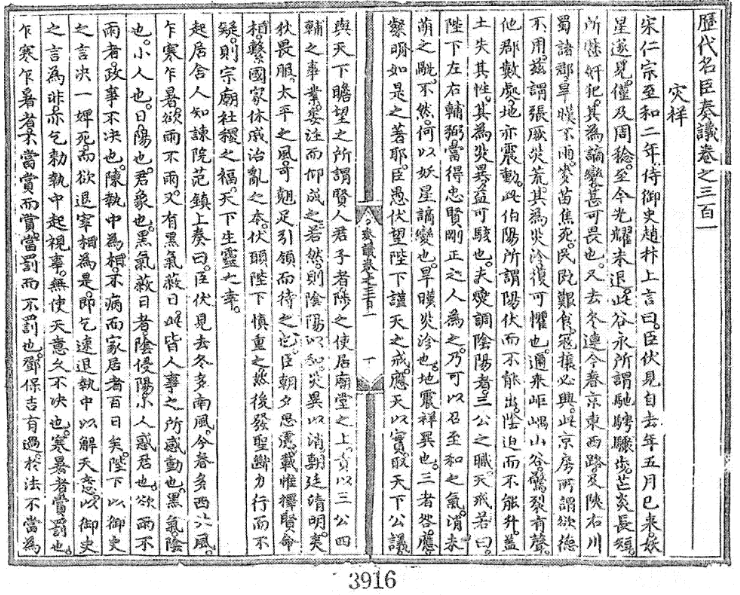
\includegraphics[width=0.8\textwidth]{figures/sn1054_chinese.png}}%
%   \captionof{figure}[Historical Chinese records about the Crab supernova]{Chinese records of the Lidai Mingchen Zouyi~\cite[535]{chinese_history}, which dates to 1414. The passage about the Crab Nebula supernova (SN 1054)
%   as was translated in \cite{crab_chinese}. 
%   The passage reads: \enquote{2\nd year of the Zhihe reign period of Emperor Renzong of 
%   Song [1055]; Attendant Censor Zhao Bian submitted a letter saying: \enquote{Your servant considers that, since the 5th month of last
%   year [when] the baleful star appeared, a full year has passed and until now its brilliance has not faded [lit. 'retreated']}. 
%   This is what Gu Yong meant by \enquote{its rapid movement, the variations in the length of its flaming rays, and the [asterisms] on which
%   it has trespassed successively}, as a censorious anomaly it is greatly to be feared.}.\label{fig:crab_chinese}}%
% \end{minipage}%
\begin{figure}[h]
  \centering
  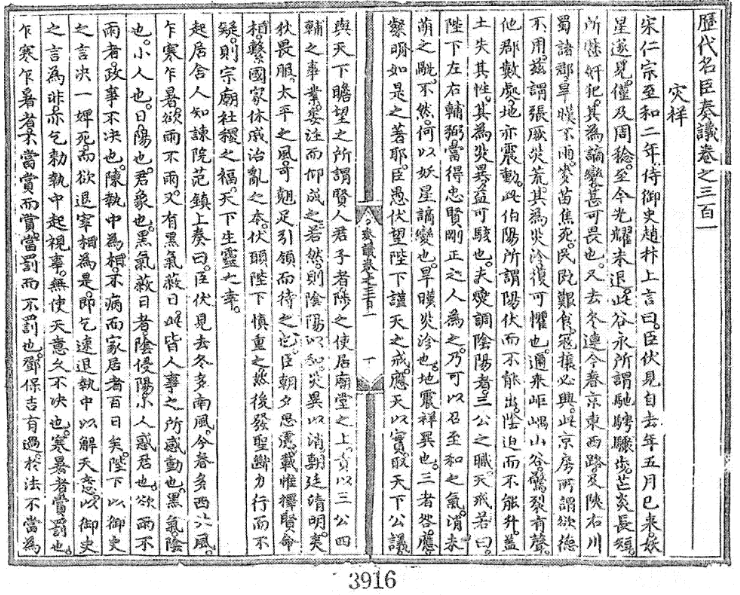
\includegraphics[width=0.8\textwidth]{figures/sn1054_chinese.png}
  % (\fontspec{Heiti SC Light}{歷代名臣奏議})
  \caption[Historical Chinese records about the Crab supernova]{Chinese records of the Lidai Mingchen Zouyi~\cite[535]{chinese_history}, which dates to 1414.
    The passage about the Crab Nebula supernova (SN 1054)as translated in \cite{crab_chinese}. 
    The passage reads: \enquote{2\nd year of the Zhihe reign period of Emperor Renzong of 
    Song [1055]; Attendant Censor Zhao Bian submitted a letter saying: \enquote{Your servant considers that, since the 5th month of last
    year [when] the baleful star appeared, a full year has passed and until now its brilliance has not faded [lit. 'retreated']}. 
    This is what Gu Yong meant by \enquote{its rapid movement, the variations in the length of its flaming rays, and the [asterisms] on which
    it has trespassed successively}, as a censorious anomaly it is greatly to be feared.}.
    }\label{fig:crab_chinese}
\end{figure}


\section{Profile Likelihood Solution}
\label{ap:wstat}
The full Poisson likelihood includes a nuisance parameter for each energy bin that describes the number of background counts.
These nuisance parameters can be removed by \enquote{profiling} the likelihood.
Solving \eqref{eq:ll_profile} for $\mu_b$ yields
\begin{equation}
  \mu_b =\frac{N_{\mathrm{off}}\alpha + N_{\mathrm{on}}\alpha - \alpha\mu_s - \mu_s - \sqrt{K}}{2\alpha(\alpha + 1)}
\end{equation}
where
\begin{equation*}
  K = \alpha^2 (N_{\mathrm{off}}^2 +  2 N_{\mathrm{off}} (N_{\mathrm{on}} + \mu_s) + N_{\mathrm{on}}^2 - 2 N_{\mathrm{on}} \mu_s + \mu_s^2) + 2 \alpha \mu_s ((N_{\mathrm{off}} - N_{\mathrm{on}}) + \mu_s) + \mu_s^2.
\end{equation*}
This expression can be substituted into \eqref{eq:full_ll} resulting in the profile likelihood which has no dependence on $\mu_b$ anymore.
Special care has to be taken when implementing this formula for zero counts in the data. 
See \url{https://docs.gammapy.org/0.11/stats/fit_statistics.html} for some information about edge cases.


\newpage
\section{Implementation for \pymc and \theano}
\label{ap:sampler_details}
The higher the sampling rate, the quicker the fit. Spending some time to optimize the code to integrate the spectral model brings a large speed improvement.
The listing below shows how the trapezoidal operation is implemented in a vectorized way using the \numpy~\cite{numpy} library.

\begin{minipage}{\textwidth}
\begin{mdframed}[backgroundcolor=white!20!black,leftmargin=0cm,rightmargin=0cm, skipabove=0pt, innerleftmargin=0,innerrightmargin=0,]
\begin{pythonlst}[basicstyle=\lstsansserif]
  # Define x and delta x. This can be pre-computed once.
  d = np.tile(np.linspace(0, 1, num=num_nodes), num_bins).reshape(num_bins, -1) 
  xs = (d * bin_widths[:, None]) + bin_edges[0:-1, None] 
  delta_xs = np.diff(xs)

  # Compute the integral of f using theano's symbolic sum operation. 
  y = f(xs, parameters)
  integral = 0.5 * theano.tensor.sum((y[:, 0:-1] + y[:, 1:]) * delta_xs, axis=1) 
\end{pythonlst}
\end{mdframed}
\end{minipage}

This unassuming piece of code brings a dramatic speed increase of at least a factor of 10. 
Instead of building single scalar gradients for each energy bin, \theano can build the Jacobian for a single tensor object. 
The gradient of the integral with respect to the parameters $N_0, \alpha, \beta$ can be build automatically. The \pymc model seems to 
sample faster when the gradients are precomputed.
Since the integral limits are constant, we can apply Leibniz integral rule~\cite{leibniz_rule} and switch the order of the differential and the integration
\begin{align*}
  \dddp{c}{\alpha} &= \ddp{\alpha} \int\limits_{\Delta \etrue} N(E; N_0, \alpha, \beta) \diff{E} = \int\limits_{\Delta \etrue} \ddp{\alpha} N(E; N_0, \alpha, \beta) \diff{E} \\
  &= \int\limits_{\Delta \etrue} \ddp{\alpha} N_0 \biggl( \frac{E}{E_0} \biggr)^{-\alpha -\beta \log_{10}\left(\frac{E}{E_0}\right)} \diff{E} \\
  &= -N_0 \int\limits_{\Delta \etrue} \biggl(\frac{E}{E_0} \biggr)^{-\alpha -\beta \log_{10}\bigl(\frac{E}{E_0}\bigr)} \log\biggl(\frac{E}{E_0}\biggr) \diff{E}.
\end{align*}
Equivalently for $\beta$
\begin{equation*}
  \dddp{c}{\beta} = -\int\limits_{\Delta \etrue} \frac{1}{\log(10)} \log^2\left(\frac{E}{E_0}\right) \biggl( \frac{E}{E_0} \biggr)^{-\alpha -\beta \log_{10}\left(\frac{E}{E_0}\right)}  \diff{E}
\end{equation*}
and last but not least the amplitude parameter $N_0$
\begin{equation*}
  \dddp{c}{N_0} =  \int\limits_{\Delta \etrue} \biggl( \frac{E}{E_0} \biggr)^{-\alpha -\beta \log_{10}\left(\frac{E}{E_0}\right)} \diff{E}.
\end{equation*}
The \pymc model can now be sampled at a rate of several hundred samples per second. The listing below shows the definition of the \pymc model.
The full code can be accessed at \github{tudo-astroparticlephysics/ll_experiments}.

\begin{minipage}{\textwidth}
  \begin{mdframed}[backgroundcolor=white!20!black,leftmargin=0cm,rightmargin=0cm, skipabove=0pt, innerleftmargin=0,innerrightmargin=0,]
  \begin{pythonlst}
  amplitude = pm.HalfFlat('amplitude')
  alpha = pm.HalfFlat('alpha')
  beta = pm.HalfFlat('beta')

  mu_s = forward_fold_log_parabola(integrator, amplitude, alpha, beta, observations)
  mu_b = pm.TruncatedNormal(
      'mu_b',
      lower=0,
      shape=len(off_data),
      mu=off_data,
      sd=5
  )

  pm.Poisson('background', mu=mu_b, observed=off_data, shape=len(off_data))
  pm.Poisson(
    'signal',
     mu=mu_s + exposure_ratio * mu_b,
     observed=on_data,
     shape=len(on_data)
  )
  \end{pythonlst}
  \end{mdframed}
\end{minipage}

\section{Sensitivity and Effective Area for Fixed On Region}
\label[app]{ap:fixed}
The sensitivity curve~\ref{fig:sensitivity} and the effective area plot~\ref{fig:eff_area_optimized} were calculated on an optimized subset of the data. 
Combinations of prediction threshold, multiplicity, and on-region radius were tested to find the best sensitivity.
This might introduce biases and \emph{over-fitting} effects since no independent test data is available. 
To mitigate the effects to some degree, the size of the on-region, $\theta$, is defined in terms of angular resolution. 
This reduces the dimension of the optimization problem and increases runtime drastically.
\begin{figure}
  \centering
  \includegraphics[width=\textwidth]{build/effective_area_optimized_fixed_theta.pdf}
  \caption[Effective area for fixed values of $\theta$]{  
    Effective area for optimized event selection in multiplicity and prediction threshold. The on-region radius $\theta$ was fixed to 
    \SI{50}{\percent} containment of the angular distance between true and estimated position in each energy bin. 
    In comparison to the results shown in \cref{fig:eff_area_optimized}, the values match the reference curve better.
  }
  \label{fig:eff_area_fixed}
  \vspace*{\floatsep}% https://tex.stackexchange.com/q/26521/5764
  \includegraphics[width=\textwidth]{build/sensitivity_fixed.pdf}
  \caption[Sensitivity curve for fixed values of $\theta$]{  
    Sensitivity curve for optimized event selection in multiplicity and prediction threshold. The on-region radius $\theta$ was fixed to 
    \SI{50}{\percent} containment of the angular distance between true and estimated position in each energy bin. 
    The results are slightly worse than the ones shown in \cref{fig:sensitivity}, but still well within the expected performance range.
  }
  \label{fig:sensitivity_fixed}
\end{figure}


\section{Dependency Graph}
The \cref{fig:dep_graph} below shows the dependency of this document. It was created from the Makefile 
by the tool \texttt{makefile2graph}\footnote{\url{https://github.com/lindenb/makefile2graph}} written by Pierre Lindenbaum. 
The output was processed with the \texttt{Gephi}~\cite{gephi} software. \texttt{Gephi} is a graphical user interface to 
modify graphs for visualization. It supports various layout algorithms and search queries in large graphs.
The figure below represents only a part of the dependency graph as one of the nodes calls into yet another Makefile recursively.
Still, the figure summarizes most data dependencies needed for a proper CTA analysis. Managing this complicated construction by hand 
would be a herculean task. I urge anyone performing data analysis of any kind to use a workflow automation tool like \make or \snakemake.

\noindent%
\begin{minipage}{\linewidth}% to keep image and caption on one page
\makebox[\linewidth]{%        to center the image
  \includegraphics[width=0.6\textwidth]{figures/make_graph.pdf}}
\captionof{figure}[Dependency Graph]{The dependency graph of this document as seen by \make. The inner nodes correspond to the final targets. 
The final pdf file, which is this very document, has the largest degree of all nodes in this graph. Unfortunately, this figure itself cannot 
be created without human interaction and cannot be created fully automatically.  
\label{fig:dep_graph}}%      only if needed  
\end{minipage}


\chapter{Configuration Files}
\label{ap:config}

\section{Configuration for the \aicttools}
\label{ap:aict_config}

The listing below shows the contents of the configuration file used for the \aicttools.
I'd like to take this opportunity and apologize for the terrible name of the \aicttools project.  
I was put on the spot by an approaching deadline and the creative fumes of the day were eluding me. 

\begin{spacing}{0.5}
  \lstinputlisting[basicstyle=\tiny\lstsansserif, multicols=2, language=yaml]{./configs/aict/iact_config.yaml}
\end{spacing}

\section{\python Requirements}
\label{sec:requirements}
I relied heavily on open-source software for every step presented in this thesis.
The most important libraries are listed below in no particular order.
\begin{itemize}
  \item \astropy~\cite{astropy_2013,astropy_2018}
  \item \numpy~\cite{numpy}
  \item \pandas~\cite{pandas}
  \item \sklearn~\cite{sklearn}
  \item \matplotlib~\cite{matplotlib}
  \item \scipy~\cite{scipy}
\end{itemize}

This document itself was built with MacTex-2018 on both macOS Mojave and macOS High Sierra.
% I did not test this on either Windows or Linux 
% \enquote{it should work}.
%  However the listing below shows the required \python packages
The listing below shows all the \python packages and their version numbers which were used to produce the results shown in this document.
given that the \python installation is properly set
\begin{spacing}{0.5}
  \lstinputlisting[basicstyle=\tiny\lstsansserif, multicols=2, language=yaml]{./build/requirements.txt}
\end{spacing}

\section{Configuration for Preprocessing}
\label{ap:preprocess_config}

The listing below shows the contents of the configuration file used for the preprocessing 
of the simulated CTA data. The list of telescope IDs selects the telescopes belonging to 
the so-called HB9 layout of the southern CTA site.

\begin{spacing}{0.6}
  \lstinputlisting[basicstyle=\footnotesize\lstsansserif, language=yaml]{./configs/preprocessing/config.yaml}
\end{spacing}
\newpage

\backmatter

\chapter*{Acknowledgements}

My deepest gratitude goes to Prof.\,Dr.\,Dr. Wolfgang Rhode for giving me the opportunity to 
work in the field of astroparticle physics and for supervising this thesis.
I also thank my second supervisor Prof.\,Dr. Kevin Kröninger for his interest in my research topic.

This work would never have been possible without the continuous support of my fellow colleagues and friends in the 
astroparticle physics group at Dortmund. It truly is a thoroughly pleasant environment to work in. 
Special thanks go out to Jens Buss, for essentially recruiting me and being the moral compass of the department, 
Lena Linhoff, for enduring my prolonged presence in her office, and Alexander Sandrock, for guiding me through horrible integral transforms.
In particular, I'd like to thank my office mate and physics partner-in-crime Maximilian Nöthe. Thanks for teaching 
me innumerable things about \python, \LaTeX and programming in general, not to mention my appreciation for active-noise-canceling technology. 
I'd like to give special thanks to everyone who took on the daunting task of 
proofreading this document: Lena Linhoff, Maximilian Nöthe, and Linda Richerd. 

Finally I can't help but acknowledge the Sonderforschungsbereich 876 for its funding 
and for giving me the opportunity to travel and meet all the terrific people that make up the CTA consortium.
A special thanks to the SFB for allowing me to work at the CEA institute in Paris during the early stages of my graduate studies.
Thanks to Thierry Stolarczyk for hosting me at CEA, Karl Kosack 
for many helpful discussions and supporting open science for CTA, and the entire group at CEA. 

I owe additional gratitude to all my friends and family who did not get to see me much during the last few months. 
In particular I'd like to thank Hannah for putting up with my late-night antics and unusual dinner schedule.


\listoffigures
\listoftables
\cleardoublepage

\begingroup
\renewcommand*{\bibfont}{\small}
\setstretch{1}
\setlength\bibitemsep{6pt}
\emergencystretch=1em
\printbibliography[heading=bibintoc]
\endgroup

  

\end{document}
